
\documentclass{article}
% ----------------------------------------------------------------
\usepackage{natbib,amsmath,amsthm,amsfonts,amssymb,fancyhdr}
\usepackage{Sweave} %
\usepackage{graphicx}
\usepackage[section]{placeins}
\usepackage[flushleft]{threeparttable}
\usepackage{pdflscape}


\setcounter{tocdepth}{4}

\newcommand{\pd}[2]{\frac{\partial #1}{\partial #2}}
\newcommand{\lap}[2]{\frac{\partial^2 #1}{\partial #2^2}}
\newcommand{\mean}{\text{mean}}

%% Change margins
\addtolength{\oddsidemargin}{-.875in}
\addtolength{\evensidemargin}{-.875in}
\addtolength{\textwidth}{1.75in}
\addtolength{\topmargin}{-.875in}
\addtolength{\textheight}{1.75in}
%%

\begin{document}
\Sconcordance{concordance:FLBEIA_manual.ltx:FLBEIA_manual.Rnw:%
1 89 1}


\title{Technical manual for \texttt{FLBEIA} a \texttt{R} package to conduct Bio-Economic Impact assessments using \texttt{FLR} (version 1.15)}

\author{Dorleta Garc\'ia, Ra\'ul Prellezo, Sonia S\'anchez, Marga Andr\'es, Agurtzane Urtizberea \\ \& Itsaso Carmona}

%\date{}
\date{\today}

\maketitle

\abstract{\texttt{FLBEIA} (FL Bio-Economic Impact Assessment) is an \texttt{R} package build on top of \texttt{FLR} libraries. The purpose of the package is to provide a flexible and generic simulation model, also called FLBEIA, to conduct Bio-Economic Impact Assessments of harvest control rule based on management strategies under a Management Strategy Evaluation (MSE) framework. The model is divided into two main blocks, the operating model (OM) and the management procedure model (MPM). The OM is formed by the biological, the fleet and the covariates components and the MPM by the observation, the assessment and the management advice components.The model is multistock, multifleet and seasonal, and uncertainty is introduced by means of montecarlo simulation. The algorithm has been coded in a modular way to ease its checking and to make it flexible. 
The package provides functions that describe the dynamics of the different model components and the user chooses which of the functions are used in each specific case study. Furthermore, for some of the components, if the functions provided within \texttt{FLBEIA} do not fulfill the requirements of a specific case study, the user can code the functions that describe better the dynamics of those components. Therefore, due to the wide choice of functionality and flexibility that provides the model, we can define it as a framework more than as a model. Main limitations of the model are that 
the stocks must be age structured or aggregated in biomass (length structure is not allowed), and that spatial dimension is not considered explicitly. However, spatial characteristics could be modeled assigning stocks and/or fleets/metiers to specific areas.
}


\newpage

\tableofcontents
\clearpage{\pagestyle{empty}\cleardoublepage}



\section{Introduction}

The idea of \texttt{FLBEIA} comes from the similarities between the different models developed to perform bio-economic analysis in AZTI-Tecnalia. These models were pieces of code re-written in order to match with the specific case study or fishery. These pieces, in many cases, reflected exactly the same processes with similar dynamics that had to be slightly adapted to the different case studies. Therefore, in order to ease the job of the modelers, we decided to develop not a model but a framework in which a model is built. This model can be constructed combining already existing functions or developing new functions and combining them with existing ones. The choice of the kind of model to be used in a specific case study depends on the questions asked, which implies that not any model can be considered valid for all purposes.

Big advances have been done the last years in the field of bio-economic modelling with the development of models such as, Fishrent \citep{Salz2011}, Fcube \citep{Ulrich2011}, FcubeEcon \citep{Hoff2010} among others, and with the development of also some theoretical and partial assessments. However, until now there is no an universal model that can be applied to address all fishery management issues. Thus, we developed \texttt{FLBEIA} with the objective to integrate many of the models available in a common bio-economic impact assessment framework as a package of FLR \citep{Kell2007} in \citep{R2010}. \texttt{FLR} \citep{Kell2007} was built with the goal of developing a common framework to facilitate collaboration within and across disciplines (e.g. biological, ecological, statistical, mathematical, economic, and social) and, in particular, to ensure that new modelling methods and software are more easily validated and evaluated, and more widely available once developed.

The package \texttt{FLBEIA} contains the model called \texttt{FLBEIA}, a collection of functions and new \texttt{S4} classes developed to facilitate the simulation  of fishery systems in response to different types of management strategies. The model allows the evaluation of different management strategies, in a wide variety of case studies and scenarios, under Management Strategy Evaluation framework \citep{Butterworth1999, Butterworth2007, Delamare1998, Punt2007, Rademeyer2007}, and identifies the potential economic and biological consequences of a proposed policy action. 

The main characteristics of \texttt{FLBEIA} package are:

\begin{itemize}

	\item	It is coded in a generic, flexible and extensible way.
	\item Provides functions to condition the simulations, to run them and to analyze the results.

\end{itemize}	

In fact, a mayor effort has been set on the second functionality, namely the simulation model.

The main characteristics of the \texttt{FLBEIA} simulation model are:
\begin{itemize}
	
	\item The model is fully biological-economic coupled and provides fully integrated bio-economic assessment.
	\item The model deals with multi-species, multi-fleet and multi-\textit{metier} situations.
	\item The model can be run using seasonal steps (smaller or equal to one year).
	\item	It is generic, flexible and extensible.
  \item Uncertainty can be introduced in almost any of the parameters used.
	
\end{itemize}

A conceptual diagram of the model is  
shown in Figure~\ref{fig:MSE_diagram}. The simulation is divided in two main blocks:
the Operating Model (OM) and the Management Procedure Model (MPM). The OM is the part of the 
model that simulates the real dynamics of the fishery system and the MPM is the part of the model that simulates the whole management process. 

\begin{figure}[ht]
  \centering
    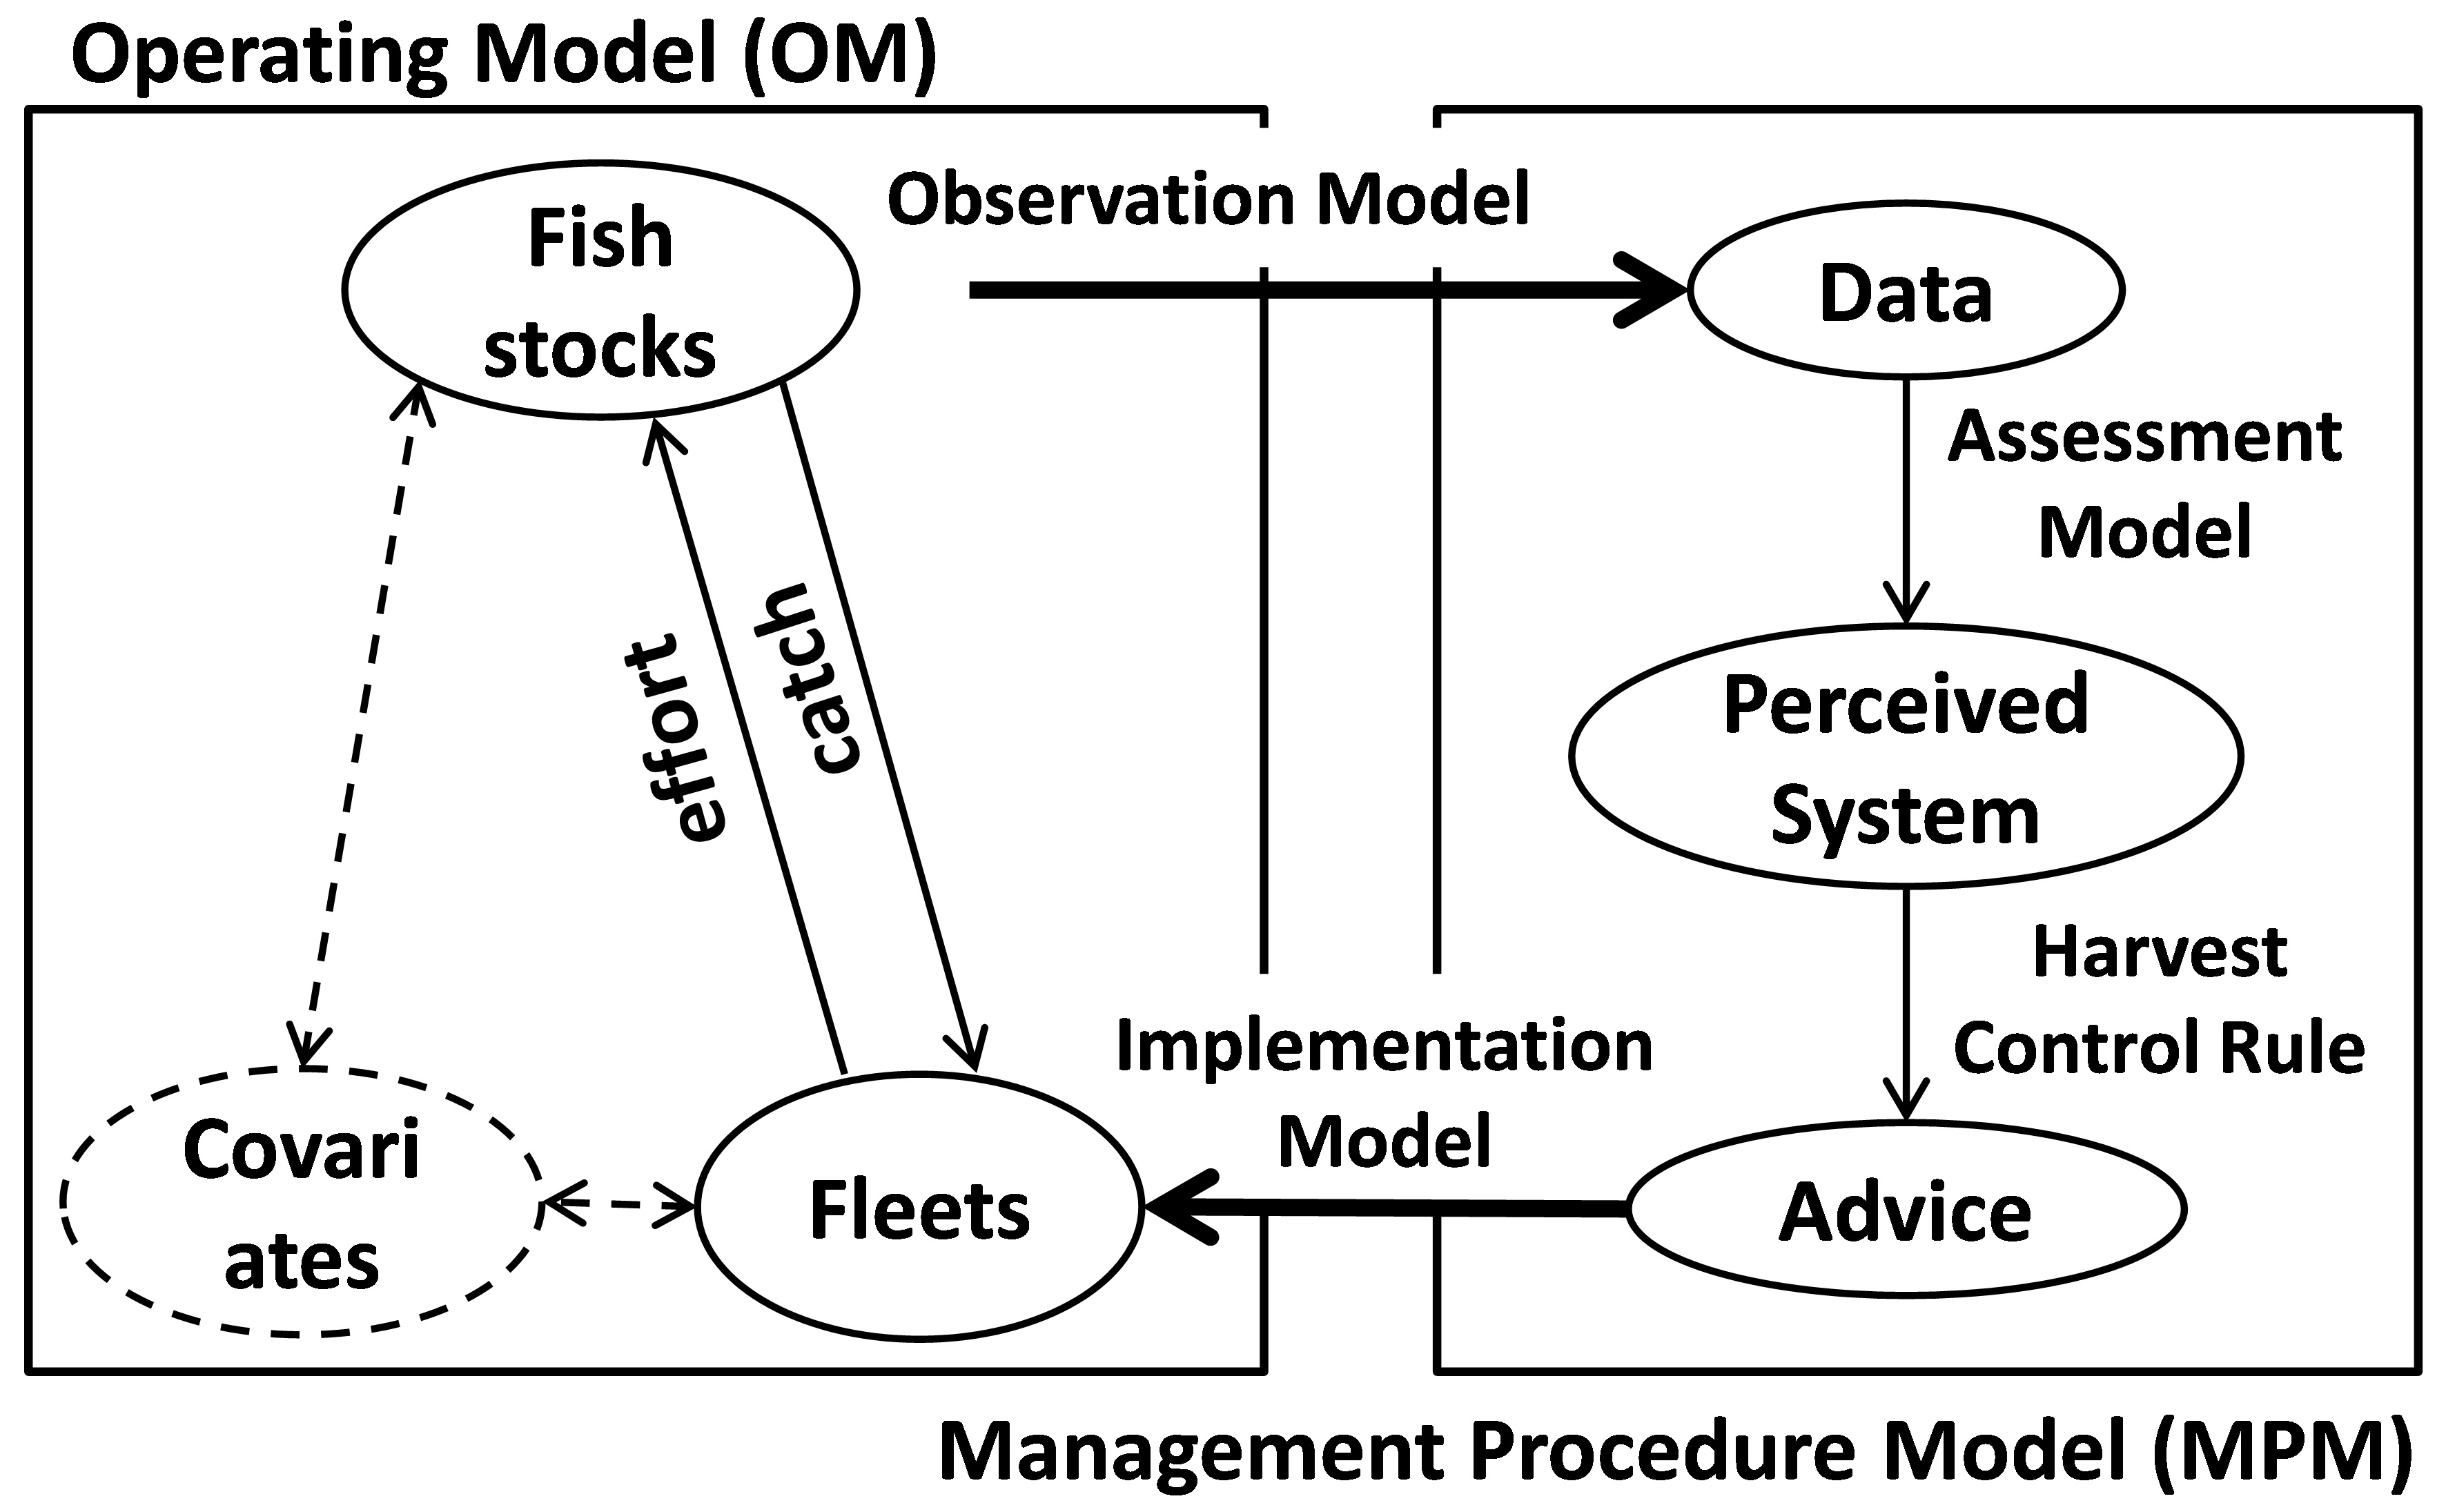
\includegraphics[width= 0.9\textwidth]{MSE_diagram}
  \caption{Conceptual representation of the main components modelled in FLBEIA. Source: \citep{Garcia2013}}
  \label{fig:MSE_diagram}
\end{figure}

The OM has three components that can interact among themselves:

\begin{enumerate}
	\item The biological populations or stocks.
  \item The fleets. 
  \item The covariates. They can be of any nature; environmental, economical or technical.
\end{enumerate}

The MPM has also three components:
\begin{enumerate}
	\item The data collected from the OM. 
  \item The observed population obtained through the application of a set of assessment models to the observed data. 
  \item The management advice obtained from the application of harvest control rules (HCR) to the observed populations.
\end{enumerate}
 

The model is built modularly with a top-down structure that has, at least, four levels:
 
\begin{enumerate}
	\item In the first level (top level), there is only one function, \texttt{FLBEIA} function. 
	It calls the functions on the second level in a determined order and it links the main components	(stocks, fleets, covariates, data, observed population and management advice) of the OM and MPM.
	
	\item The functions in the second level correspond with the generation of each of the components in the Figure~\ref{fig:MSE_diagram}. The OM components project the objects one season forward: \texttt{biols.om} projects the stocks, \texttt{fleets.om} projects the fleets and \texttt{covars.om} projects the covariates. The MPM components generate the objects necessary to produce the management advice, they generate the objects based on OM objects and they operate at most once a year: \texttt{observation.mp} generates the data, \texttt{assessment.mp} generates the observed population and \texttt{advice.mp} generates the management advice. They take the input objects and return only those related to the component they belong to.
			
	\item The functions in the third level define the specific dynamics of each component 
	and they are chosen by the user in each simulation. They are always called by a second level function and in some cases, a third level function also calls fourth level functions. For example a function that describes the dynamics of an age structured population can call a stock recruitment function. In this way, a function used	to describe age structured populations can be combined with different stock recruitment relationships.  
  
	\item The functions in the fourth level are called by functions in the third level and are used to model the most basic processes in the simulation. They are coded as a function and selected by the user because it could be interesting to use the same third level function together with different fourth level functions, as in the case of age structured population and stock recruitment functions.
	
	 \end{enumerate}
	 
This top down structure allows avoiding the classical structure of separated biological and economic (and social) modules (that could be integrated or not). Therefore, when the model is designed and the modeler takes the decision of including a particular characteristic, it does not make any difference if the characteristic is biological or economical, only matters at which level the characteristic is.

\texttt{FLBEIA} framework permits to incorporate new third and lower level functions or to modify them, while first and second level ones are fixed. Changing first or second level functions would imply a different approach, but the existing third and lower level functions would be useful.

In the next Sections \texttt{FLBEIA}'s conceptual model and its specifications are explained. Firstly, in Section~\ref{sec:FLBEIAconcept}, the conceptual model characterizes the main components as well as the feedbacks and loops among them. Secondly, in Section~\ref{sec:FLBEIArun}, it is explained how to run FLBEIA to perform MSE. Thirdly, in Section~\ref{sec:FLBEIAfun}, the model specification describes the components, the currently available functions by level, and how to use them within the \texttt{FLBEIA} package. Next, in Section~\ref{sec:FLBEIASmartCond}, a way to easily condition the model is presented. And finally, in Section~\ref{sec:FLBEIAoutput}, the \texttt{FLBEIA} function output is described.



\section{The concept of \texttt{FLBEIA}} \label{sec:FLBEIAconcept}

  The simulation model is divided in two main blocks, the Operating Model (OM) and the Management Procedure Model (MPM). This division is part of 
  the requirements of the MSE approach, that is, the model includes a mathematical representations of the \textit{real world} (OM), the 
  \textit{observed world} (MPM) and the interactions between them.


\subsection{Operating model}

  The OM is the part of the model that simulates the real dynamics of the fishery system. It is divided in three components or operating models, 
  the biological, the fleets and the covariates operating model. It runs in seasonal time steps, and it projects the components in each time step. 
  Firstly, it updates the biological component, secondly the fleet component and finally the covariates component.

\paragraph{Biological component} \hspace{0pt} \smallskip

  The biological component simulates the population dynamics of the stocks. The number of populations is, in principle, unlimited. 
  The limitation could come from memory problems with \texttt{R} and/or the operating system. The stocks can be described as age structured
  populations or as biomass dynamics populations, since length structured populations models are not supported by the simulation algorithm. 
  Each stock can follow a different population dynamics model and is projected independently. It does not mean that they  cannot be interdependent 
  between them but the order in which  these biological components are updated has to be decided and it will affect the results obtained.

\paragraph{Fleet component} \hspace{0pt} \smallskip

  The fleet component simulates the behaviour and dynamics of the individual fleets. As the number of the stocks, the number of fleets is in 
  principle unlimited. The limitation could come from memory problems with \texttt{R} and/or the operating system used. The activity of the fleets is divided into metiers. The metiers are formed by trips that have the same catchability for all the stocks. 
  Fleet fishing effort and effort share among metiers are independently updated for each fleet in each season. Fleet catchability and/or capacity is updated annually, independently for each fleet, through capital dynamics according to its own economic performance. 

\paragraph{Covariates component} \hspace{0pt} \smallskip

  This part of the model incorporates all the variables that are not part of the biological or fleet components and that affect any of the operating model components or the management process. The number of covariates is, in principle, unlimited. The limitation could come from memory problems with \texttt{R} and/or the operating system used.

\paragraph{Links among and within components} \hspace{0pt} \smallskip

  The links within the OM components are not restricted by the general settings of the simulation model. Therefore, it is the user who decides 
  which are the links that should be included in the model. The possible links that can be included are:

  \begin{itemize}
  	\item The link within the \textsl{biological} component, where catch affects abundance.
  	\item The link within the \textsl{fleets} component, where fleet capacity affects fishing effort. 
  	\item The link between the \textsl{biological and fleets} components, where fishing effort and fish abundance affects catches. 
  \end{itemize}

 
\subsection{Management procedure model}

  The Management Procedure Model (MPM) is divided into 3 components: the observation, the assessment and the management advice. The observation 
  component produces the required data to run the assessment. Then, the assessment component is applied to those data to obtain the observed 
  populations. Finally, the management advice component produces a management advice based on the observed populations. MPM procedure is applied 
  yearly in the appropriate season of the year. Not necessarily in the last season, for example, it can be simulated as in the case of anchovy in 
  the Bay of Biscay, where management is applied from the mid-season of one year to the mid-season of the next year. Simulations with multi-annual 
  advice is also possible.

\paragraph{Observation component} \hspace{0pt} \smallskip

  The observation component generates the required objects to run the assessments. Three types of objects can be generated:
  
  \begin{itemize}
  	\item Stocks. 
  	\item Fleets. 
  	\item Abundance indices.
  \end{itemize}
  
  Stocks and abundance indices objects are generated independently, stock by stock, whereas fleets are observed jointly. 
  These objects are generated based on the variation that is introduced in the components of the OM. This variation can be due to:
  
  \begin{itemize}
  	\item Introducing uncertainty to the OM variables, or
  	\item adjusting the OM variables to the assessment model requirements which is going to be used in the next step (e.g. collapsing the dimensions -age, season,...), or
  		\item adjusting the OM variables to the legal conditionings (TACs, quotas, TAE, discards,...).
  \end{itemize}
 
\paragraph{Assessment component} \hspace{0pt} \smallskip

  Assessment models are applied on a stock by stock basis and they can vary from stock to stock.

\paragraph{Management advice component} \hspace{0pt} \smallskip

  The management advice component produces a set of indicators (determined by the user) useful for policy making.
  The management advice is produced based on the output obtained from the observation and assessment components.
  The advice is first applied at single stock level and after that it can be applied at fleet level. 



\section{Running \texttt{FLBEIA}} \label{sec:FLBEIArun}

\subsection{Input objects}

  \texttt{FLBEIA} requires some input arguments to run a simulation. There are two types of arguments: the main arguments, which give information on 
  the stocks, the fleets and the covariates, and the control arguments, which control the behaviour of the main and the second level functions 
  (see Section~\ref{sec:2ndlvl}). The main arguments contain biological information on the stocks (\texttt{biols}, \texttt{SRs} and 
  \texttt{BDs}), information on the fleets (\texttt{fleets}), additional variables (\texttt{covars}) and information on management 
  (\texttt{indices}, \texttt{advice}). Regarding the control arguments, there is a control object related to the main function 
  \texttt{FLBEIA} (\texttt{main.ctrl}), whereas the others relate to the main arguments (\texttt{biols.ctrl}, \texttt{fleets.ctrl}, 
  \texttt{covars.ctrl}, \texttt{obs.ctrl}, \texttt{assess.ctrl}, \texttt{advice.ctrl}).
  For detailed information on the input objects required see Section~\ref{sec:1stlvl}.
  
  In order to easy the creation of the objects with the appropriate object format some additional functions has been implemented to create the inputs 
  (see Section~\ref{sec:SmartCondFun}). Additionally, several examples has been coded for guidance (see Section~\ref{sec:SmartCondEx}).
  
\subsection{Main function: \texttt{FLBEIA}}

  To perform biological and economic simulations it is necessary to invoke the main function, \texttt{FLBEIA}, which calls to different subfunctions 
  to perform the simulations depending on the control elements set.
  
  \noindent \texttt{FLBEIA} function is called as follows:
  
  \begin{center}
    \texttt{FLBEIA(biols, SRs, BDs, fleets, covars, indices, advice, 
            main.ctrl, biols.ctrl, fleets.ctrl, covars.ctrl, obs.ctrl, assess.ctrl, advice.ctrl) }
	\end{center}
  
  For more details on the \texttt{FLBEIA} function see Section~\ref{sec:1stlvl}.

\subsection{Output object}

  The output of \texttt{FLBEIA} function is a list containing information on the expected evolution of the fish stocks (\texttt{biols}), the fleets 
  (\texttt{fleets}), the covariates (\texttt{covars}), the provided advice (\texttt{advice}), the assessed stocks and observed indices 
  (\texttt{stocks} and \texttt{indices}), the control elements for the fleets (\texttt{fleets.ctrl}) and the versions of the different packages
  used to run the simulations (\texttt{pkgs.versions}). All the elements except \texttt{stocks} and \texttt{pkgs.versions} correspond with the
  updated versions of the objects used in the call to FLBEIA. 
  
  \noindent It has the following structure:
  \begin{center}
    \texttt{list(biols='FLBiols', fleets='FLFleetsExt', covars='FLQuants', advice='list(TAC,TAE,quota.share)', 
            stocks='FLStocks', indices='FLIndices', fleets.ctrl='list', pkg.versions='matrix') }
  \end{center}
  
  \noindent Description of the outputs:
    \begin{description}
      \item[\texttt{biols}:] \texttt{FLBiols} object containing historical and future "real" evolution of the stock.     
      \item[\texttt{fleets}:] \texttt{FLFleetsExt} object containing historical and future "real" evolution of the fleets 
  regarding effort exerted, distribution among m\'etiers, catches, prices and so on.
      \item[\texttt{covars}:] Named list containing historical and future evolution of the different covariates.     
      \item[\texttt{advice}:] List containing information on management advice (e.g. TAC,TAE,quota.share).     
      \item[\texttt{stocks}:] Named list with one element per stock of class \texttt{FLStock} or \texttt{NULL}, if a \texttt{FLStock} is not needed to run the assessment.
          Contains the perceived stocks used in the management procedure to produce the management advice.
          For details on \texttt{FLStock} object see Figure~\ref{fig:FLStock}.
      \item[\texttt{indices}:] Named list with one element per stock of class \texttt{FLIndices} or \texttt{NULL}, if a \texttt{FLIndices} is not needed to run the assessment. 
      \item[\texttt{fleets.ctrl}:] Control object used for the \texttt{fleets.om} function.
      \item[\texttt{pkgs.versions}:] Matrix indicating the packages and package version used along the simulation.
    \end{description}



\section{\texttt{FLBEIA} functions} \label{sec:FLBEIAfun}

\subsection{First level function: \texttt{FLBEIA}} \label{sec:1stlvl}

	\texttt{FLBEIA} function is a multistock, multifleet and seasonal simulation algorithm coded in a generic, flexible and extensible way. It is generic because it can be applied to any case study that fit into the model restrictions. The algorithm is made up by third and fourth level functions specified by the user. In addition of the existing functions new ones can be defined and used if necessary. This is why we define the model as flexible and extensible. 
	
	To determine the simulation, the third- and fourth-level functions must be specified in the main function \texttt{FLBEIA}. For this purpose it has a control argument associated to each second level function. These control arguments are lists which include the name of the functions to be used in the simulations and any extra argument required by those functions that is not already contained in the main arguments. 
	
\noindent \texttt{FLBEIA} function is called as follows:

\begin{center}
  \texttt{FLBEIA(biols, SRs, BDs, fleets, covars, indices, advice, 
        main.ctrl, biols.ctrl, fleets.ctrl, covars.ctrl, obs.ctrl, assess.ctrl, advice.ctrl) }
\end{center}

\noindent Main arguments:
\begin{description}
	\item[\texttt{biols}:] An \texttt{FLBiols} object (list of \texttt{FLBiol} objects). The object must be named and the names must be the same as in the \texttt{SRs} object, the \texttt{BDs} object and the \texttt{catches} slots within \texttt{FLFleetExts} object. For details on \texttt{FLBiol} object see Figure~\ref{fig:FLBiol}. 
	\item[\texttt{SRs}:] A list of \texttt{FLSRsim} objects. This object is a simulation version of the original \texttt{FLSR} object. The object must be named and the names must be the same as in the \texttt{FLBiols} object. For details on \texttt{FLSRsim} object see Figure~\ref{fig:FLSRsim}.
	\item[\texttt{BDs}:] A list of \texttt{FLBDsim} objects. This object is similar to \texttt{FLSRs} object but oriented to simulate	population growth in biomass dynamics populations. The object must be named and the names must coincide with those used in \texttt{FLBiols} object. For details about \texttt{FLBDsim} object see Figure~\ref{fig:FLBDsim}.
	\item[\texttt{fleets}:] An \texttt{FLFleetsExt} object (list of \texttt{FLFleetExt} objects). \texttt{FLFleetExt} object is almost equal to the original \texttt{FLFleet} object but the \texttt{FLCatch} object in \texttt{catch} slot has been replaced by \texttt{FLCatchExt} object. The difference between  \texttt{FLCatch}  and \texttt{FLCatchExt} objects is that \texttt{FLCatchExt} has two extra slots \texttt{alpha} and \texttt{beta} used to store Cobb-Douglas production function parameters, $\alpha$ and $\beta$, \citep{Cobb1928, Clark1990}. $\alpha$ corresponds with the exponent of effort and $\beta$ to the exponent of biomass. The \texttt{FLFleetsExt} object must be named and these names must be consistently used in the rest of the arguments. For details about \texttt{FLFleetExt} object see Figure~\ref{fig:FLFleetExt}.
	\item[\texttt{covars}:] An \texttt{FLQuants} object. This object is not used in the most basic configuration of the algorithm. Its content depends on the third or lower level functions that make use of it.  
	\item[\texttt{indices}:] A list of \texttt{FLIndex} objects. Each element in the list corresponds with one stock. The list must be named and the names must be the same as in the \texttt{FLBiols} object. For details about \texttt{FLIndex} object see Figure~\ref{fig:FLIndex}.
	\item[\texttt{advice}:] A list. The class and content of its elements depends on two functions, the function in \texttt{fleet.om} defined to simulate fleets' effort and the function used to produce advice in \texttt{advice.mp}. 
\end{description}
   
   
\noindent Control arguments:
\begin{description}
	\item[\texttt{main.ctrl}:]   Controls the behaviour of the main function, \texttt{FLBEIA}. 
	    For details on \texttt{main.ctrl} object see Table~\ref{tb:A3.table1}. 
	\item[\texttt{biols.ctrl}:]  Controls the behaviour of the second level function \texttt{biols.om}. 
	    For details on \texttt{biols.ctrl} object see Table~\ref{tb:A3.table2}.
	\item[\texttt{fleets.ctrl}:] Controls the behaviour of the second level function \texttt{fleets.om}. 
	    For details on \texttt{fleets.ctrl} object see Table~\ref{tb:A3.table3}.
	\item[\texttt{covars.ctrl}:] Controls the behaviour of the second level function \texttt{covars.om}. 
	    For details on \texttt{covars.ctrl} object see Table~\ref{tb:A3.table4}.
	\item[\texttt{obs.ctrl}:]    Controls the behaviour of the second level function \texttt{observation.mp}. 
	    For details on \texttt{obs.ctrl} object see Table~\ref{tb:A3.table5}.
	\item[\texttt{assess.ctrl}:] Controls the behaviour of the second level function \texttt{assessment.mp}. 
	    For details on \texttt{assess.ctrl} object see Table~\ref{tb:A3.table6}.
	\item[\texttt{advice.ctrl}:] Controls the behaviour of the second level function \texttt{advice.mp}. 
	    For details on \texttt{advice.ctrl} object see Table~\ref{tb:A3.table7}.
\end{description}



\subsection{Second level functions} \label{sec:2ndlvl}

	\subsubsection{Biological component: \texttt{biols.om}}
	
	The call to the function within \texttt{FLBEIA} is done as:
	
	\begin{center}
		\texttt{biols.om(biols, fleets, SRs, BDs, covars, biols.ctrl, year, season)}
	\end{center}
		
		This function projects the stocks one season forward. The projection is done independently stock by stock by the third level function specified for each stock in \texttt{biols.ctrl} object. Currently, there are three population dynamics functions implemented, one corresponding to age structured populations, \texttt{ASPG}, the second one to biomass dynamics populations, \texttt{BDPG} and another one to fixed populations (given as input), \texttt{fixedPopulation}. These functions do not include predation among stocks, but this kind of models could be implemented and used in the algorithm if necessary.

  \noindent Control arguments:
  \begin{description}
    \item[\texttt{biols.control}:] This argument is a list which contains the necessary information to run the third level functions that are called by \texttt{biols.om}. The elements depend on the third and lower level functions used to describe the 	dynamics of the stocks. The list must contain at least one element per stock and the name of the element must coincide exactly with the name used in $\texttt{biols}$ argument so it can be used to link the population with its dynamics model. At the same time, each of these elements must be a list with at least one element, \texttt{growth.model}, which specifies the name of the function used to describe population dynamics (options: \texttt{ASPG}, \texttt{BDPG} or \texttt{fixedPopulation}).
    
  	For example:
       
    \begin{Schunk}
      \begin{Sinput}
        > biols.ctrl
      \end{Sinput}
      
      \begin{Soutput}
        $NHKE
        $NHKE$growth.model
        [1] "ASPG"
        
        $CMON
        $CMON$growth.model
        [1] "BDPG"
        
        $FAKE
        $FAKE$growth.model
        [1] "ASPG"
      \end{Soutput}
    \end{Schunk}
  \end{description}

	
	\subsubsection{Fleets component: \texttt{fleets.om}}
		
		The call to \texttt{fleets.om} function within \texttt{FLBEIA} is done as:
		
		\begin{center}
			\texttt{fleets.om(fleets, biols, covars, advice, fleets.ctrl, advice.ctrl, year, season) }
		\end{center}

	This function projects the fleets one season forward. 
 	The main argument, \texttt{fleets}, is an object of class \texttt{FLFleetsExt} (for more detail see Section~\ref{sec:1stlvl})
  %, an extension of the \texttt{FLFleet} object. The difference is in the \texttt{catches} slot that in the case of 
	%\texttt{FLFleetsExt} object is of class \texttt{FLCatchesExt}.  \texttt{FLCatchExt} objects 
	% are equal to the original \texttt{FLCatch} but has 2 extra slots, \texttt{alpha} and
	%\texttt{beta}. These two slots have been added to store Cobb-Douglas production function parameters.
	
	The function is divided in three processes related to fleet dynamics: the effort model, the price model and the capital model.
	Effort and capital models are fleet specific, whereas price model is fleet and stock specific.
	First, \texttt{fleets.om} calls the effort model and it updates the slots related to 
	effort and catch. The effort models are called independently fleet by fleet. Then, \texttt{fleets.om}
	calls the price model in fleet by fleet and stock by stock basis, which updates the \texttt{price} slot
	in the \texttt{fleets} object. Finally, but only in the last season of the year, the function calls the capital model. 
  Thus, investment and disinvestment is only done annually. 
	The capital model is called independently fleet by fleet. 
	
\begin{description}
	\item[Effort model:] This part of the model simulates the tactical behaviour of the fleet every season and iteration.
	 In each time step and iteration, the effort exerted by each individual fleet and its effort-share among metiers is 
	 calculated depending on the stock abundance, management restrictions or others. 
	 After that, the catch produced by the combination of effort and effort-share
	 is calculated and \texttt{discards, discards.n, landings, landings.n} slots are filled.
	 Other stored variables in \texttt{fleets.ctrl} could also be updated here, for example \texttt{quota.share},
	 as a result of the exerted effort. 
	 
	 The effort model is specified at fleet level, so each fleet can follow a different effort model.
	 At the moment there are 4 functions available: \texttt{fixedEffort, SMFB, SSFB} and \texttt{MaxProfit}. 
	 To write new functions for effort, it must be taken into account that the input arguments 
	 must be found among \texttt{fleets.om} function arguments and that the output must be a 
	 list with updated \texttt{FLFleetsExt} and \texttt{fleets.ctrl} objects, i.e.:
				
  \begin{Schunk}
    \begin{Sinput}
    list(fleets = my_fleets_obj, fleets.ctrl = my_fleets.ctrl_obj)
    \end{Sinput}
  \end{Schunk}	 	
		
			 	  
	\item[Price Model:] The price model updates the price-at-age at stock, metier and fleet level in each time
	step and iteration. 
	
	At the moment, there are 2 functions available: 
	\texttt{fixedPrice} and \texttt{elasticPrice}. 
	To write new functions for price it must be taken into account that the input arguments 
	must be found among \texttt{fleets.om} function arguments and that the output must be a 
	list with an updated \texttt{FLFleetsExt} object.
				
	\item[Capital Model:] This module is intended to simulate the strategic behaviour of the fleets, namely, the investment and disinvestment dynamics. 
	The model is applied at fleet level and in an annual basis and can affect fleets'  
	capacity and  catchability. Catchability could be modified through investment in technological improvement 
	and capacity as a result of an increase (investment) or decrease (disinvestment) in the number of vessels.  
	Changes in fleets' capacities could produce a variation in quota share among fleets, for example.
	Thus, the corresponding change would have to be done in \texttt{fleets.ctrl} object. 
	
	At the moment, there are 2 functions available: \texttt{fixedCapital} and \texttt{SCD}.
	To write new functions for capital dynamics, as for effort and price, it must be taken into account 
	that the input arguments must be found among \texttt{fleets.om} function arguments and that the 
	output must be a list with updated \texttt{FLFleetsExt} and \texttt{fleets.ctrl} objects.				
\end{description}


\noindent Control arguments:
\begin{description}
  \item[\texttt{fleets.ctrl}:] The most simple example of fleet dynamics model and hence 
  	the most simple \texttt{fleets.ctrl} object correspond with the model where all the parameters 
		in \texttt{fleets} object are given as input and maintained fixed
		 within the simulation. This is obtained using the third level functions, \texttt{fixedEffort, fixedPrice} and
		 \texttt{fixedCapital} which do not need any extra arguments. In the case of two fleets,
		 \texttt{FL1} and \texttt{FL2}, where \texttt{FL1} catches 3 stocks, \texttt{ST1, ST2} and \texttt{ST3} and \texttt{FL2}
		 catches  \texttt{ST1} and \texttt{ST3} stocks, the \texttt{fleets.ctrl} could be created using the following code:
     
  \begin{Schunk}
    \begin{Sinput}
    >fleets.ctrl <- list()
    
    # The fleets
    >fleets.ctrl[['FL1']] <- list()
    >fleets.ctrl[['FL2']] <- list()
    
    # Effort model per fleet.
    >fleets.ctrl[['FL1']]$effort.model <- 'fixedEffort'
    >fleets.ctrl[['FL2']]$effort.model <- 'fixedEffort'
    
    # Price model per fleet and stock.
    >fleets.ctrl[['FL1']][['ST1']]$price.model  <- 'fixedPrice'
    >fleets.ctrl[['FL1']][['ST2']]$price.model  <- 'fixedPrice'
    >fleets.ctrl[['FL1']][['ST3']]$price.model  <- 'fixedPrice'
    
    >fleets.ctrl[['FL2']][['ST1']]$price.model  <- 'fixedPrice'
    >fleets.ctrl[['FL2']][['ST3']]$price.model  <- 'fixedPrice'
    
    # Capital model by fleet.
    >fleets.ctrl[['FL1']]$capital.model  <- 'fixedCapital'
    >fleets.ctrl[['FL2']]$capital.model  <- 'fixedCapital'
    
    > fleets.ctrl
    \end{Sinput}
    \begin{Soutput}
      $FL1
      $FL1$effort.model
      [1] "fixedEffort"
      
      $FL1$ST1
      $FL1$ST1$price.model
      [1] "fixedPrice"
      
      $FL1$ST2
      $FL1$ST2$price.model
      [1] "fixedPrice"
      
      $FL1$ST3
      $FL1$ST3$price.model
      [1] "fixedPrice"
      
      $FL1$capital.model
      [1] "fixedCapital"
       
      $FL2
      $FL2$effort.model
      [1] "fixedEffort"
      
      $FL2$ST1
      $FL2$ST1$price.model
      [1] "fixedPrice"
      
      $FL2$ST3
      $FL2$ST3$price.model
      [1] "fixedPrice"
      
      $FL2$capital.model
      [1] "fixedCapital
    \end{Soutput}
  \end{Schunk}
\end{description}

 
	\subsubsection{Covariates component: \texttt{covars.om}}
	
	\texttt{covars.om} projects \texttt{covars} object one season forward.  
	\texttt{covars} object is a named list and the class and dimension of each element will depend 
	on the function used to project it into the simulation. 
	
	\noindent The call to \texttt{covars.om} function within \texttt{FLBEIA} is done as:

  \begin{center}
    \texttt{covars.om(biols, fleets, covars, advice, covars.ctrl, year, season) }
  \end{center}

	Internally, for each element in the \texttt{covars} list, it calls to the third level functions
	specified in the \texttt{covars.ctrl} object. At the moment, there exist 2 third level functions: \texttt{fixedCovar}, 
	which is used to work with variables that are input parameters not updated within the simulation and \texttt{ssb.get}, 
  which is used to get the real Spawning Stock Biomass of one of the simulated stocks. 
	
	The economic variables used in the capital dynamics model \texttt{SCD} should be stored in 
\texttt{covars} object and updated in each step using values in \texttt{fleets} object.

\noindent Control arguments:
\begin{description}
  \item[\texttt{covars.ctrl}:] This argument is a named list with one element per covariate and the names of the list must match those used 
  to name the \texttt{covars} object. Each of the elements is, at the same time, a list with, at least, one element, \texttt{dyn.model}, 
	which defines the dynamics of the covariate in question (options: \texttt{fixedCovar}, \texttt{ssb.get}).
\end{description}

	This way of working could be useful, for example, for environmental variables such as 
	sea surface temperature that could affect catchability or recruitment in the fleet and 
	biological operating models respectively and that are external to fishery system. 
	
	A covariate with a non-trivial 
	dynamics could be the abundance of certain animal which is not commercially exploited by the fleet, but which abundance
	affects the natural mortality of any of the exploited stocks. In this case, 2 extra functions will be needed, the function
	that defines the dynamics of the covariate and the function that models the natural mortality of the stock as a function of the abundance
	of the animal. The first function should be declared in \texttt{covars.ctrl} argument and the former one in 
	\texttt{biols.ctrl} argument as a stock dynamics model. 
 
	
	\subsubsection{Observation component: \texttt{observation.mp}}
	
	The observation component generates the necessary data to run the assessment models.
	The main function is \texttt{observation.mp} and it calls third level functions 
	which generate 3 possible objects, a \texttt{FLStock}, a \texttt{FLIndices} or a 
	\texttt{FLFleetsExt} object. The \texttt{FLStock} and  \texttt{FLIndices} objects
	are generated independently for each stock and the \texttt{FLFleetsExt} object
	jointly for all the fleets.
	
	\noindent The call to \texttt{observation.mp} function within \texttt{FLBEIA} is done, stock by stock, as follows:
	
  \begin{center}
  	\texttt{observation.mp(biols, fleets, covars, indices, advice, obs.ctrl, year, season, stknm) }
  \end{center}

  \noindent where \texttt{stknm} is the name of the stock to be observed and its name matches with those used in the \texttt{biols} object.
  
	The output of \texttt{observation.mp} is a list with 3 elements. The first element, \texttt{stock} is an object 
	of class \texttt{FLStock} or \texttt{NULL}, if a \texttt{FLStock} is not needed to run the assessment.
	The second element, \texttt{indices}, is a named list with one element per stock and its names correspond with those used 
	in \texttt{biols} object. The elements of the \texttt{indices} list are   
	of class  \texttt{FLIndices} or \texttt{NULL}, if a \texttt{FLIndices} is not needed to run the assessment.    
	The third element, \texttt{fleets.obs}, is an observed version of the original \texttt{fleets} object.
	At the moment, there is no third level function implemented to generate observed fleets.
  %The segmentation of the fleet in the observed version would be different to the real one.

% +++++ SONIA: NECESARIO REPASAR Y CORREGIR SIGUIENTE PARRAFO (se espera actualizacion por necesidades para anchoa) +++++

	As the management process is currently run in a yearly basis, the \texttt{unit} and \texttt{season}
	dimensions are collapsed in all the observed objects. Moreover, if the management process is being conducted at the end of year \texttt{y} the observed objects extend up to year \texttt{y-1}, 
  whereas they extend up to year \texttt{y} in the cases when management process is conducted in any other season as it happens in reality.
		
\noindent Control arguments:
\begin{description}
  \item[\texttt{obs.ctrl}:] %This argument is a list with one element per stock. If fleets were observed 
  	%the object should have also one element per fleet but as at the moment there are no functions that provide
		%observed version of \texttt{FLFleetsExt} object this option is not described here.
		The \texttt{obs.ctrl} object must be a named list where the names used correspond with 
		those used in the \texttt{FLBiols} object. Each stock element is, at the same time, a list 
		with two elements (\texttt{stkObs} and \texttt{indObs}) and these two elements are once again lists. 
		A scheme of \texttt{obs.ctrl} object is presented in Table~\ref{tb:A3.table5}.

  	The \texttt{stkObs} element is a list with the arguments necessary to run the 
		third level function used to generate the \texttt{FLStock} object. In the list there must be 
		at least one element, \texttt{stkObs.model}, with the name of the third level function 
		that will be used two generate the \texttt{FLStock} object. If it is not required to generate a \texttt{FLStock} 
		object, then \texttt{NoObsStock} value should be assigned to \texttt{stkObs.model} argument and 
		this function will return the \texttt{NULL} object.

		The \texttt{indObs} element is a list with one element per index in the \texttt{FLIndices} object.
		Each element of the list is, at the same time, a list with the arguments necessary to run the 
		third level function used to generate the \texttt{FLIndex} object. In the list there must be 
		at least one element, \texttt{indObs.model}, with the name of the third level function 
		that will be used two generate the \texttt{FLIndex} object. If it is not required to generate a \texttt{FLIndices} 
		object, then \texttt{indObs} element will be set equal to \texttt{NoObsIndex} instead of a list and this will return 
		the \texttt{NULL} object instead of a \texttt{FLIndices} for the corresponding stock.

\end{description}


	\subsubsection{Assessment component: \texttt{assessment.mp}}
	
	The assessment component applies an existing assessment model to the stock data objects generated by the observation model 
	(\texttt{FLStock} and \texttt{FLIndices}). The assessment models are applied stock by stock, independently.
	
	\noindent The call to \texttt{assessment.mp} function within \texttt{FLBEIA} is done as follows:
	
  \begin{center}
  	\texttt{assessment.mp(stocks, fleets.obs, indices, assess.ctrl, datayr, stknm)}
  \end{center} 
  
  \noindent where \texttt{stknm} is the name of the stock to be assessed and its name corresponds with one of those used 
  in the \texttt{biols} object.

	The output of the function is a list of \texttt{FLStocks} with \texttt{harvest}, \texttt{stock.n} and \texttt{stock}
	slots updated. Within \texttt{FLBEIA} no new assessment models are provided, but the models already available in \texttt{FLR}
	can be used. 

\noindent Control arguments:
\begin{description}
  \item[\texttt{assess.ctrl}:] This argument is a named list with one element per stock, where the names must coincide with those
  used in the \texttt{biols} object. The elements must have at least one element, \texttt{assess.model}, which defines the name of 
	the assessment model to be used for each stock. Furthermore, if the assessment model to be used is non-trivial 
	(i.e. different to \texttt{NoAssessment}), the list must contain a second argument  \texttt{control} with the adequate control object
	to run the assessment model.
\end{description}

	
	\subsubsection{Management advice component: \texttt{advice.mp}}
	
	The management advice component generates an advice based on the output of assessment and/or observation components.  
	
	\noindent The call to \texttt{advice.mp} function within \texttt{FLBEIA} is done, stock by stock, as follows:

  \begin{center}	
  	\texttt{advice.mp(stocks, fleets.obs, indices, covars, advice, advice.ctrl, year, season, stknm)}
  \end{center}
  
  \noindent where \texttt{stknm} is the name of the stock to be assessed and its name correspond with one of those used 
  in the \texttt{biols} object.

	% NOTA (SONIA): EN ESTOS MOMENTOS EL CONSEJO SE GENERA INDEPENDIENTEMENTE STOCK POR STOCK, SIN POSIBILIDAD DE CONSEJO CONJUNTO!
  % (DEBEMOS PLANTEAR UNA SOLUCION SI HAY INTENCION DE USAR EL ENFOQUE FCube)
  %First, the advice is generated stock by stock, independently. Later a function that generates advice based on the single 
	%stock advices, observed fleets and others could be applied, \texttt{FCube} like approaches \citep{Ulrich2011}. 
	The output of the function is an updated \texttt{advice} object.
	
	Depending on the structure of the third level functions used to generate advice and to simulate fleet dynamics, the
	advice could be an input advice (effort, temporal closures, spatial closures -implicitly through changes in catchability-...)
	or an output advice (catch).  

\begin{description}
  \item[\texttt{advice}:] The structure of \texttt{advice} object is open and it is completely dependent on the
  third level functions used to describe fleet dynamics and to generate the advice. For example, if \texttt{SMFB}
	and \texttt{annualTAC} are used to describe fleet dynamics and generate the advice respectively, then \texttt{advice}
	is a list with two elements, \texttt{TAC} and \texttt{quota.share}. \texttt{TAC} is an annual \texttt{FLQuant} 
	with the \texttt{quant} dimension used to store stock specific TACs and, \texttt{quota.share} is a named list with one
	element per stock being the elements \texttt{FLQuant}-s with  \texttt{quant} dimension used to 
	store fleet specific annual quota share.
\end{description}

\noindent Control arguments:
\begin{description}
  \item[\texttt{advice.ctrl}:] This argument is a named list with one element per stock and one more element for each fleet.
  The names must coincide with those used to name \texttt{biols} object and the name of the extra argument must be \texttt{fleets}.
	The elements of the list are, at the same time, lists with at least one element, \texttt{HCR.model}, with the name of the model used to 
	generate the single stock and fleet advice depending on the case.     
\end{description}



\subsection{Third level functions}

%~~~~~~~~~~~~~~~~~~~~~~~~~~~~~~~~~~~~~~~~~~~~~~~~~~~~~~~~~~~~~~~~~~~~~~~~~~~~~~~~~~~~~~~~~~~~~~~~~~~~
%----------------------------------------------------------------------------------------------------	
\subsubsection{Population growth functions}
%~~~~~~~~~~~~~~~~~~~~~~~~~~~~~~~~~~~~~~~~~~~~~~~~~~~~~~~~~~~~~~~~~~~~~~~~~~~~~~~~~~~~~~~~~~~~~~~~~~~~

  The following population growth functions are currently defined:
%----------------------------------------------------------------------------------------------------	

\paragraph{\texttt{fixedPopulation}: Fixed population function} \hspace{0pt} \smallskip
%----------------------------------------------------------------------------------------------------
		
	In this function all the parameters are given as input, 
  because there is not any population dynamics simulated.
  For the stocks for which we select its dynamics as fixed population, 
  natural mortality (i.e. \texttt{biols[[stock.name]]@m}) has to be set equal to 0 
  and additionally, if the population is aggregated in biomass, biomass growth (i.e. \texttt{BDs[[stock.name]]@gB}) 
  has also to be set equal to 0.


\paragraph{\texttt{ASPG}: Age Structured Population Growth function} \hspace{0pt} \smallskip
%----------------------------------------------------------------------------------------------------
		
	The function \texttt{ASPG} describes the evolution of an age structured population using an 
	exponential survival equation for existing age classes and a stock-recruitment 
	relationship to generate the recruitment. The recruitment can occur in one or more seasons.	
	However, the age is measured in integer years and the seasonal cohorts are tracked 
	separately. The seasonal cohorts and their corresponding parameters are stored in 
	the '\texttt{unit (u)}' dimension of the \texttt{FLQuant}-s. And all the individuals 
	move from one age group	to the following one in the 1st of January.  Thus, being
	$\phi$ the recruitment function, $RI$ the reproductive index, 
	$N$ the number of individuals, $M$ the natural mortality,  
	$C$ the catch, $a_0$ the age at recruitment, $s_0$ the season when the recruitment
	was spawn, and $a$, $y$, $u$, $s$ the subscripts for age, year, unit  
	and season respectively, the population dynamics can be written mathematically as:
			
	If $s = 1$,
		
			\begin{equation}
				N_{a,y,u,1} = \left\{ 
				\begin{array}{l l}
	 				\phi\left( RI_{y = y-a_0, s = s - s_0}	\right) 					& \text{, } a = a_0\\ % RECRUITMENT
	 				(N_{i_a}\cdot e^{-\frac{M_{i_a}}{2}} - C_{i_a}) % MIDDLE AGES
	 				\cdot e^{-\frac{M_{i_a}}{2}}	& \text{, } a_0 < a < A\\ 
	 				% PLUSGROUP	
	 				(N_{i_{A-1}}\cdot e^{-\frac{M_{i_{A-1}}}{2}} - C_{i_{A-1}})\cdot e^{-\frac{M_{i_{A-1}}}{2}} + \\
	 				(N_{i_A}\cdot e^{-\frac{M_{i_A}}{2}} - C_{i_A})\cdot e^{-\frac{M_{i_A}}{2}}  & \text{, } a = A\\
	 				\end{array} \right.
		  \end{equation}
		
	\noindent where $i_a = (a-1,y-1,u,ns)$, $i_{A-1} = (A-1,y-1,u,ns)$ and  $i_A = (A,y-1,u,ns)$.
    
  If $s > 1$,
		
		\begin{equation}
			N_{a,y,u,s} = \left\{ 
				\begin{array}{l l}
	 			\phi\left( RI_{y = y-a_0, s = s - s_0}	\right) 					& \text{, } a = a_0\\ % RECRUITMENT
	 			% AGES > REC
	 			(N_{i_a}\cdot e^{-\frac{M_{i_a}}{2}} - C_{i_a}) \cdot e^{-\frac{M_{i_a}}{2}}	& \text{, } a_0 < a \leq A\\
	 		\end{array} \right.
		\end{equation}
		
	\noindent where $i_a = (a, y, u, s-1)$.
    
  And the reproductive index $RI$ is  given by:

		\begin{equation}
		 	RI_{y-a_0,s} = 	\sum_a \sum_u (N \cdot wt \cdot mat \cdot fec 
		 	                \cdot exp-(M \cdot M_{spwn}+F \cdot F_{spwn}))_{a,y-a_0,u,s}
		\end{equation}
		
	\noindent where $wt$ is the mean weight, $mat$ is the percentage of mature individuals, 
	                $fec$ is the fecundity parameter, 
	                $M_{spwn}$ and $F_{spwn}$ are the proportion of natural and fishing mortality, respectively, 
	                occurring before spawning.

	The stock-recruitment relationship $\phi$ is specified in the \texttt{model} slot of corresponding 
	\texttt{FLSRsim} object. \texttt{FLSRsim} object enables modeling a great variety of stock-recruitment relationships depending 
	on its functional form and seasonal dynamics. Details on available stock-recruitment relationships are given in Section~\ref{sec:SRR}.
	
	
\paragraph{{\texttt{BDPG}: Biomass Dynamics Population Growth function}} \hspace{0pt} \smallskip
%----------------------------------------------------------------------------------------------------

	The function \texttt{BDPG} describes the evolution of a biomass dynamics population, i.e. a population with no 
  age, stage or length structure. The population is aggregated in biomass, $B$, and the growth of the population, $g$
  is a function of the current biomass and the catch $C$. The model is mathematically described in Equation~\ref{eq:BDPG}: 
	
	\begin{equation}
		B_{s,y} = \left\{ 
				\begin{array}{l l}
	 					B_{s-1,y}  + g(B_{s-1,y}) - C_{s-1,y}  & \text{, } s \neq 1\\
	 					B_{ns,y-1} + g(B_{ns,y-1}) - C_{ns,y-1}& \text{, } s = 1
  			\end{array} \right.
  	\label{eq:BDPG}
	\end{equation}
  
  \noindent where $s$ and $y$ are the subscripts for age and year, respectively, and $ns$ is the number of seasons.
	As \texttt{FLBEIA} is seasonal, the equation also depends on the season. The growth model $g$ and its parameters are 
	specified, respectively, in the \texttt{model} and \texttt{params} slot of corresponding \texttt{FLBDsim} class.  
	Currently only Pella and Tomlinson model \citep{Pella1969} is	implemented to model growth, but new models can be defined if needed.
	
	The following parameterization of the growth model has been implemented:
	
	\begin{equation}
		g(B) = B\cdot \frac{r}{p}\cdot\left[1-\left(\frac{B}{K}\right)^p\right]
	\end{equation}
  
  \noindent where $r$ is the intrinsic rate of population increase, $K$ the carrying capacity and $p$ the assymetry parameter.
  Additionally, there has been added a restriction in order to avoid negative values.
  This arises when population is at high biomass values (well above carrying capacity) 
  and outside the range of observed biomass levels in the past. 
  Moreover, it doesn't occur for larger catches that result in lower biomass levels. 
  Intuitively, this seemed to be contradictory because the population collapsed in the absence of catches case 
  and remained stable for higher catch levels. 
  Therefore, in the absence of catches, we restrict the biomass to be $\alpha$ times the carrying capacity 
  ($B_t \leq \alpha \cdot K$). 
  In other words, $B_t = min(B_t, \alpha \cdot K)$. But note that:
   $$ \alpha \geq 1 $$
   $$ \alpha \leq \left(\frac{p}{r}+1\right)^{\frac{1}{p}}$$
	Note that when we introduce stochasticity in the parameters of the Pella-Tomlinson model 
	(e.g. from a Bayesian model or from a bootstrapping) we have a range of values for the surplus production model. 
	So that $\alpha$ must be smaller than the minimum value across iterations: $\alpha \leq min_i((p_i/r_i+1)^{1/p_i})$.
  The value of $\alpha$ has to be introduced by the user in the \texttt{BDs[[stock.name]]@alpha}.
  Above restrictions will be checked in \texttt{FLBEIA} and it will print an error if they are not fullfilled.
  Finally, note that these restrictions arise from the no catch case. 
  So, even after restricting the biomass, there might be cases when some levels of catches lead to negative biomasses. 

  When working with populations structured in biomass, the biomass values has to be stored in the \texttt{*.n} slots, whereas \texttt{*.wt} slots has to be set to 1.

%----------------------------------------------------------------------------------------------------
%~~~~~~~~~~~~~~~~~~~~~~~~~~~~~~~~~~~~~~~~~~~~~~~~~~~~~~~~~~~~~~~~~~~~~~~~~~~~~~~~~~~~~~~~~~~~~~~~~~~~
\subsubsection{Effort models}
%~~~~~~~~~~~~~~~~~~~~~~~~~~~~~~~~~~~~~~~~~~~~~~~~~~~~~~~~~~~~~~~~~~~~~~~~~~~~~~~~~~~~~~~~~~~~~~~~~~~~
%----------------------------------------------------------------------------------------------------	

  The following effort model functions are currently defined:

\paragraph{\texttt{fixedEffort}: Fixed effort model} \hspace{0pt} \smallskip
%----------------------------------------------------------------------------------------------------

	  In this function all the parameters are given as input except discards and landings 
	(total and at age). The only task of this function is to update the discards and landings (total and at age)
	according to the catch production function specified in \texttt{fleets.ctrl} argument.
		
	Two arguments need to be declared as elements of \texttt{fleets.ctrl} if this function is used, \texttt{effort.model = 'fixedEffort'} 
	and \texttt{catch.model}. The last argument is used to specify the catch production function that will be used to generate the catch. 
  Note that first argument must be declared at fleet level (i.e \texttt{fleets.ctrl[[fleet.name]]\$effort.model}), 
  second argument at fleet and stock level (i.e. \texttt{fleets.ctrl[[fleet.name]][[stock.name]]\$catch.model})
	and that catch production model corresponds with a fourth level function. For more details see Section~\ref{sec:CprodFun}.
		
		
\paragraph{\texttt{SMFB}: Simple Mixed Fisheries Behaviour model} \hspace{0pt} \smallskip
%----------------------------------------------------------------------------------------------------

		This model is a simplified version of the behavior of fleets that work in a 
	mixed fisheries framework. The function is seasonal and assumes that effort share among metiers is
	given as input parameter.
	 
	In each season, the effort of each fleet, $f$, is restricted by the seasonal landing quotas or catch quotas
	of the stocks that are caught by the fleet. Additionaly, the option of Landing Obligation (LO) is included. 
	The following steps are followed in the calculation of effort:
	

\begin{enumerate}
	
	\item Compare the overall seasonal quotas, $\sum_f Q_{f,s,st}\cdot TAC$, with the abundances of the stocks.
		 If the ratio between overall quota and abundance exceeds the 
		seasonal catch threshold, $\gamma_{s,st}$, reduce the quota share in the same degree. Mathematically: 
		
	\begin{equation}
		Q'_{f,s,st} = 
			\begin{cases}
			 		Q_{f,s,st}	     & \text{, if }  \frac{\sum_f Q_{f,s,st}\cdot TAC}{B_{s,st}} \leq \gamma_{s,st}\\
   					Q_{f,s,st}\cdot \frac{B_{s,st}\cdot \gamma_{s,st}}{\sum_f Q_{f,s,st}\cdot TAC}   & \text{, otherwise} 
			\end{cases} 
	\end{equation}
		
  \item According to the catch production function, calculate the efforts corresponding to the landing or 
		catch quotas, $Q'_{f,s,st}\cdot TAC$, of the  
		individual stocks, $\left\{ E_{f,s,st_1},\ldots, E_{f,s,st_n} \right\}$.
	
	\item Based on the efforts calculated in the previous step, calculate an unique effort, $E_{f,s}$. 
		To calculate this effort the following options can be used:
		\begin{description}  
			\item[\texttt{max}:] The maximum among possible efforts, $\hat{E}_{f,s} = \max_{j=1,\ldots,n} E_{f,s,st_j}$
			\item[\texttt{min}:] The minimum among possible efforts, $\hat{E}_{f,s} = \min_{j=1,\ldots,n} E_{f,s,st_j}$
			\item[\texttt{mean}:] The mean of possible efforts, $\hat{E}_{f,s} =  \mean_{j=1,\ldots,n} E_{f,s,st_j}$
			\item[\texttt{previous}:] The effort selected is the effort most similar to previous year effort on 
				that season, 
				$$\hat{E}_{f,s} = \left\{ E_{f,s,st} :   
				\left|1 - \frac{E_{f,s,st}}{E_{f,y-1,s}}\right| = \min_{j=1,\ldots,n} \left|1 - \frac{E_{f,s,st_j}}{E_{f,y-1,s}}\right|\right\}$$
  	 	\item[\texttt{stock.name}:] The effort corresponding to \texttt{stock.name} is selected:
				$\hat{E}_{f,s} =  E_{f,s,\texttt{stock.name}}$
		\end{description}
		If  there is LO, instead of using the option chosen by the user, the option to calculate the unique effort 
		will be the minimum among possible efforts.
	
	\item When LO is applied, calculate the new effort using the exemptions and flexibilities (de Minimis, 
	  year tranfer and quota swap). 
	  \begin{itemize}
  		\item \textit{de Minimis}: The fleet is allowed to discard a percentage of the quota to increase the effort 
  		  in order to catch other stocks.
  		\item \textit{year transfer}: The fleet can borrow next year's quota to catch it in the current year.
  		\item \textit{quota swap}: A percentage of the quota of one stock can be transfered to the effort 
  		  limiting stock if two stocks are in the same group. These groups are specifiyed by the user.
	  \end{itemize}		
		
  \item Compare the effort, $\hat{E}_{f,s}$, with the capacity of the fleet, $\kappa_f$  
    (capacity must be measured in the same units as effort and it must be stored in the \texttt{capacity} slot 
    of the \texttt{FLFLeetsExt} object). 
		If the capacity is bigger, then the final effort is unchanged and if the capacity is smaller, 
		the effort is set equal to the capacity, i.e.:
	
	\begin{equation}	
			E_{f,s} =
  				\begin{cases}
  				 	\kappa_f			 & \text{, if } \kappa < \hat{E}_{f,s}\\
   					\hat{E}_{f,s}  & \text{, if } \kappa \geq \hat{E}_{f,s}
  				\end{cases}
	\end{equation}	 
	
	\item The catch corresponding to the effort selected is calculated for each stock and compared with the 
	  corresponding quota. 
		If the catch is not equal to the quota and the season is not the last one, 
		the seasonal quota shares of the rest of the seasons are reduced or increased 
		proportionally to their weight in the total share. The shares are changed 
		in such a way that the resultant annual quota share is equal to the original one.
		In case the difference between actual catch and that corresponding to the quota exceeds
		the quota left over in the rest of the seasons, the quota in the rest of the seasons is
		canceled.	Mathematically for season $i$ where $s \leq i \leq ns'$: 
		
	\begin{equation}
		Q''_{f,i,st} =  \max\left( 0,Q'_{f,i,st} + (Q'_{f,s,st} - Q''_{f,s,st}) \cdot 
		                \frac{Q'_{f,i,st}}{\sum_{j>s} Q'_{f,j,st}}\right) 
	\end{equation}
		
		\noindent where $Q'$ denotes the quota share obtained in the first step and $Q''$ the new quota share. 
	
\end{enumerate}

\subparagraph{The \texttt{fleets.ctrl} argument in \texttt{SMFB} function}
\quad\\	

	\texttt{SMFB} function requires several control arguments at global and fleet level that are described below.

  \quad\\
		Global arguments:
		\begin{description}
		
			\item[\texttt{catch.threshold}:] This element is used to store $\gamma_{s,st}$ parameter described in
				the first step of \texttt{SMFB} function algorithm. The element must be a \texttt{FLQuant} object with dimension 
		        \texttt{[stock = nstk, year = ny, unit = 1, season = ns, area = 1, iter = ni]}, where the
	            names in the first dimension must match with those used to name \texttt{FLBiols} object. 
	            Thus, the thresholds may vary between stocks, seasons, years and iterations.
	    		The elements of the object are proportions between 0 and 1 that indicate the maximum percentage of the 
	    		stock that can be caught in each season. The reason to use this argument is that it is reasonable to think
	    		that it is impossible to fish all the fish in the sea. Thus, although the TAC is very large the actual catch
	    		will be restricted to  $\gamma_{s,st}\cdot B_{s,st}$.
			
			\item[\texttt{seasonal.share}:]  A named \texttt{FLQuants} object, one per stock, with the proportion of the 
				fleets' TAC share that 'belongs' to each season, so the sum along seasons for each fleet, year and iteration
				should be equal to 1.	The elements must be \texttt{FLQuant} objects with dimension 
		        \texttt{[fleet = nf, year = ny, unit = 1, season = ns, area = 1, iter = ni]}, where the
	            names in the first dimension must match with those used to name \texttt{FLFleetsExt} object. 
	            The names of the \texttt{FLQuants} must match stock names used in the \texttt{FLBiols} object. 
		\end{description}
		
	\quad\\			
		Fleet level arguments (i.e. \texttt{fleets.ctrl[[fleet.name]]}):
    		
		\begin{description}
			\item[\texttt{effort.model}:] \texttt{'SMFB'}.
			\item[\texttt{effort.restr}:] alternative values are \texttt{'max'}, \texttt{'min'}, \texttt{'mean'}, 
			  \texttt{'previous'} or \texttt{'stock.name'} (the name of one of the stocks caught by the fleet). 
				\begin{description}
					\item[\texttt{max}:] The fleet will continue fishing until the catch quotas of all the stocks are exhausted. 
					\item[\texttt{min}:] The fleet will stop fishing when the catch quota of any of the stocks is exhausted. 
					\item[\texttt{previous}:] Among the efforts obtained under each stock restriction the effort most similar 
					  to the previous year effort will be selected. 
					\item[\texttt{stock}:] The fleet will continue fishing until the catch quota of '\texttt{stock}' is exhausted. 
					  (This could correspond, for example, with a situation where the catch of one stock is highly controlled.)								\end{description}
				These options are explained mathematically above when the \texttt{SMFB} function is described step by step. 
			  There are two alternatives: one option for all years or one option for each year (vector with the length ny).
			\item[\texttt{restriction}:] Alternative values are \texttt{'catch'} or \texttt{'landings'}. 
			  Assigned value depends on wether the efforts are calculated according to catch or landings restriction. 
			  There are two alternatives: one option for all years or one option for each year (vector with the length ny).
      \item[\texttt{LandObl}:] Logical or vector with a logic value for each year. 
        If it is \texttt{TRUE} for that year, LO rule is applied. 
        The fleet has to stop fishing when they reach the first quota of the stocks. 
        Therefore, the unique effort will be the minimum among possible efforts. 
			\item[\texttt{LandObl\_minimis}:] Vector with a logic value for each year. 
			  If it is \texttt{TRUE} for that year, \textit{de Minimis} exemption is used.
			\item[\texttt{LandObl\_yearTransfer}:] Vector with a logic value for each year. 
			  If it is \texttt{TRUE} for that year, \textit{year Transfer} flexibility is used.
			\item[\texttt{LandObl\_minimis\_p}:] Matrix with values between 0 and 1, the maximum percentage of quota that 
			  the fleet could increase for each stock in each year. 
			\item[\texttt{LandObl\_yearTransfer\_p}:] Matrix with values between 0 and 1, the maximum percentage of quota 
			  of each stock that the fleet could borrow from next year's quota. 
			\item[\texttt{LandObl\_discount\_yrTranfer}:] Matrix with values between 0 and 1. 
			  The discount to be applied if in the previous year was used that amount. 
			  This object is used to store the percentage used from the next year's quota.
			\item[\texttt{LO\_stk\_grp}:] named vector with length equal to the number of stocks, 
			  same number for the same group of stocks to swap the quotas.
    \end{description}
    
  \quad\\
		Fleet/stock level arguments (i.e. \texttt{fleets.ctrl[[fleet.name]][[stock.name]]}):
	
    \begin{description}
  		\item[\texttt{catch.model}:] The name of the fourth level function which gives the catch production 
  				given effort and biomass (aggregated or at age). The function must be coherent with \texttt{SMFB}
  				and the function used to simulate the population growth. 
  				At the moment, two functions are available	\texttt{CobbDouglasAge} and \texttt{CobbDouglasBio}.
  				For more details see Section~\ref{sec:CprodFun}.
    \end{description}


\paragraph{\texttt{SSFB}: Simple Sequential Fisheries Behaviour model} \hspace{0pt} \smallskip
%----------------------------------------------------------------------------------------------------

  Simple sequential fisheries behaviour is related to those fleets whose fishing profile changes with 
  the season of the year. \texttt{SSFB} function models the behaviour of fleets that work in a sequential 
  fisheries framework. It is assumded that, in each season, the fleet, $f$, has only one target species or 
  stock, $st$, thus the metier, $m$, is defined on the basis of the   season and target species, resulting 
  only in one target species per each metier.
  
  In each season, $s$, the effort allocated to each species, $st$, or metier, $m$, follows the historical trend (in order to capture the 
  seasonality of each species fishing season), but it is restricted to the remaining catch quota of the fleet. 
  
  Therefore, production function is applied at metier level, but the production has some restrictions, 
  in both catches, $C$, and effort, $E$, that are described through the following steps: 
  
  \begin{enumerate}
    
    \item Calculate the total quota that corresponds to each fleet, $CQ$, from the historical data and estimate remaining
    quota for the fleet, $RQ_{s,f,st}$, deducting the catches from previous seasons.
  					$$RQ_{s,f,st} = CQ_{f,st} - \sum_{ss<s} {C_{ss,f,st}} = TAC \cdot QS_{f,st} - \sum_{ss<s} {C_{ss,f,st}}$$
    \noindent Where $QS$ is the quota share and $C$ the catches.
    
    \item Compare the total remaining quotas with the abundances of the stocks. If the ratio between remaining quotas and
    abundance exceeds the seasonal catch thershold, $\gamma_{s,st}$, then reduce the remaining quota the same amount.
    		\[
     			RQ'_{s,f,st} = \begin{cases}
       							RQ_{s,f,st} & \text{, if } \frac {\sum_f Q_{s,f,st}}{B{s,st}} \leq \gamma_{s,st}; \\
       							RQ_{s,f,st} \cdot  \frac{B{st,s} \cdot \gamma_{s,st}} {\sum_{f} RQ_{s,f,st}} & \text{, otherwise.} 
                     \end{cases}
    		\]
		
    \item Initially expected effort, $\hat E_{s,f}$, is shared between different metiers (i.e. species) month by month
    on the basis of historical seasonal effort pattern.
    				$$\hat E_{s,m,st} = \hat E_{s,f} \cdot E_{s,m} = \kappa_f \cdot PED_{s,f} \cdot  E_{s,m}$$
    \noindent Where $E_{s,m}$ is the effort share by metier, $PED_{s,f}$ is the percentage of effective days and $\kappa_f$ is the 
    fleet's capacity.

    \item Expected catches ,$\hat C_{s,m,st}$, corresponding to that initial effort, are calculated through the Cobb-Douglas catch
    production function at metier and stock level, seasonally.
    
    \item If the expected catches resulting from the previous step are higher than the remaining quota corresponding to
    each metier (Step 2), there is extra effort which has to be reallocated among the other species.
        $$\text{If   } \hat C_{s,f,st} > RQ_{s,f,st} \Rightarrow 
                        \hat C_{s,f,st} = RQ_{s,f,st} \Rightarrow E_{s,m,st} < \hat E_{s,m,st}; $$
       	$$\text{else } \hat C_{s,f,st} \leq RQ_{s,f,st} \Rightarrow
                        \hat C_{s,f,st} = C_{s,f,st} \Rightarrow E_{s,m,st} = \hat E_{s,m,st}.$$

    \item The reallocation of remaining effort, $\hat E_{s,m,st} - E_{s,m,st}$, can be performed in different ways:
      \begin{itemize}
        \item Proportionally to the price and availability of the species in a given season, or
        \item proportionally to the effort allocated to the remaining metiers.
      \end{itemize}
    
    \item This is repeated stock by stock until no effort remains to be allocated or all the TACs are exhausted

  \end{enumerate}
  
\subparagraph{The \texttt{advice} argument in \texttt{SSFB} function}
\quad\\

  \texttt{SSFB} function requires arguments in the \texttt{advice} object as described below.

  \quad\\
  \noindent Global arguments:
  \begin{description}
  	\item \texttt{quota.share}: A named \texttt{FLQuants} object, one per stock, with the total proportion of TAC that 'belongs' to 
  		each fleet each year and dimension \texttt{[fleet = nf, year = ny, unit = 1, season = 1, area = 1, iter = ni]}. The '\texttt{fleet}' dimension names must match fleets' names. And the \texttt{FLQuants} must match stock names. 
  		For each year and iteration the sum of the proportions must be equal to 1. 
  \end{description}

\subparagraph{The \texttt{fleets.ctrl} argument in \texttt{SMFB} function}
\quad\\

  \texttt{SSFB} function requires several control arguments at global and fleet level that are described below.

  \quad\\
  \noindent Global arguments:
  \begin{description}
    \item[\texttt{catch.threshold}:] A \texttt{FLQuant} object with dimension \texttt{[stock = nst, year = ny, unit = 1, season = ns, area = 1, iter = ni]}, which contains the proportion of biomass that total catch of stock cannot exceed, i.e. the previously mentioned $\gamma_{s,st}$ parameter.
  \end{description}

  \quad\\
  \noindent Fleet level arguments (i.e. \texttt{fleets.ctrl[[fleet.name]]}):
  \begin{description}
  	\item[\texttt{effort.model}:] '\texttt{SSFB}'
  	\item[\texttt{restriction}:] '\texttt{catch}'. Related to quota threshold.
    \item[\texttt{effectiveDay.perc}:] A  \texttt{FLQuant} object with dimension \texttt{[quant = 1, year = ny, unit = 1, season = ns, area = 1, iter = ni]}, which contains the proportion of days expected to be effective in a season (i.e. in which the fleet will go out fishing), the previously mentioned $PED$ parameter (see Step 3).
  	\item[\texttt{effort.realloc}:] Alternative values are \texttt{NULL} or '\texttt{curr.eff}'. Element used to describe how does the remaining effort have to be reallocated between the rest of the metiers targeting stocks for which there is already remaining quota.
  		\begin{description}
  			\item[\texttt{NULL}:] The same proportion is assigned for all metiers.
  			\item[\texttt{curr.eff}:] Effort is reallocated proportionally to the expected effort share. 
  		\end{description}
  \end{description}
  
  \quad\\
  \noindent Fleet/stock level arguments (i.e. \texttt{fleets.ctrl[[fleet.name]][[stock.name]]}):
  \begin{description}
    \item[\texttt{TAC.OS.model}:] Function to model the TAC overshoot. 
      Currently the only available function is \texttt{TAC.OS.triangCond}, which simulates a triangular distribution function 
      for TAC overshoot, in the range \texttt{(min, max)} and a peak in the \texttt{mode}.
    \item[\texttt{TAC.OS.triangCond.params}:] A named numeric vector of dimension 3. 
      Corresponding to the parameters required by \texttt{TAC.OS.triangCond} function, \texttt{min}, \texttt{max} and \texttt{mode}.
    \item[\texttt{discard.TAC.OS}:] Logical. If \texttt{TRUE}, the TAC overshoot is discarded, in other case the TAC overshoot
      is incorporated to landings.
  \end{description}


\paragraph{\texttt{MaxProfit}: Maximization of profit under a TAC constraint model} \hspace{0pt} \smallskip
%----------------------------------------------------------------------------------------------------

This second model used to simulate \textit{mixed fisheries} dynamics calculates the total effort and the effort 
  allocation among metiers that maximises the profit of the fleet.
  The total effort is constrained by the capacity of the fleet (capacity unit has to be converted in the same unit as effort) 
  and by the catch quota of some  of the stocks. Mathematically:
                                               
    \begin{equation}\label{eq:maxprof.stkCnst}
                   \max_{E_f, \gamma_{f,1},\ldots,\gamma_{f,n_{MT,f}}} 
                    % \left[  
                      % \left( 1- crewS \right) \cdot
                      \sum_m\sum_{st}\sum_a  L_{st,a,f,m} \cdot P_{st,a,f,m}- 
                             E_f\cdot\gamma_{f,m}\cdot VaC_{f,m} - FxC_f\cdot n_{V_f}
                    % \right]
    \end{equation}

  \noindent with the constraints:

  \begin{equation}\label{eq:MP_consts}
                  \left\{
                  \begin{array}{ll}
                                 & 0 \leq \gamma_{f,m}\leq 1 \text{ and } \sum_m\gamma_{f,m} = 1\\
                                 & E_f \leq \kappa_f,\\
                                 & C_{st,f} \leq QS_{st,f} \quad \text{for } st \in \Delta_f.
  %                            & C_{st} \leq \tau \cdot B_{st} \text{for any $st$}
                  \end{array}        
                  \right.
  \end{equation}

\noindent where $P$ is the price of the fish landed, 
  $VaC$ the variable cost of fishing effort, which depends on the metier and is given as cost per unit of effort, 
  $FxC$ the fixed costs of each fishing unit, which is given at fleet level and in terms of cost per vessel,
  $n_{V}$ is the number of vessels in the fleet,
  $\kappa$ is the capacity, defined as the maximum effort that the fleet can execute in each season,
  $QS$ is fleet's TAC share and
  $\Delta$ is the set of stocks for which the constraint must be fulfilled. 
In biomass dynamic populations, landings and prices are given at stock level.

\subparagraph{The \texttt{fleets.ctrl} argument in \texttt{MaxProfit} function}
\quad\\

  \texttt{MaxProfit} function requires several control arguments at fleet level
    that are described below.

  \quad\\
  \noindent Fleet level arguments (i.e. \texttt{fleets.ctrl[[fleet.name]]}):
  \begin{description}
    \item[\texttt{stk.cnst}:] A vector with the name of the stocks that constraints the capacity 
       of the fleet (i.e. maximum effort that fleet can execute in each season) 
       given the catch quota of these stocks.  
    
  \end{description}

  \quad\\
  \noindent Fleet/stock level arguments (i.e. \texttt{fleets.ctrl[[fleet.name]][[stock.name]]}):
  \begin{description}
    \item[\texttt{TAC.OS.model}:] Function to model the TAC overshoot. 
      Currently the only available function is \texttt{TAC.OS.triangCond}, which simulates a triangular distribution function 
      for TAC overshoot, in the range \texttt{(min, max)} and a peak in the \texttt{mode}.
    \item[\texttt{TAC.OS.triangCond.params}:] A named numeric vector of dimension 3. Corresponding to the parameters required by \texttt{TAC.OS.triangCond} function, \texttt{min}, \texttt{max} and \texttt{mode}.
    \item[\texttt{discard.TAC.OS}:] Logical. If \texttt{TRUE}, the TAC overshoot is discarded, in other case the TAC overshoot
      is incorporated to landings.
  \end{description}


\paragraph{\texttt{MaxProfitSeq}: Maximization of profit under a TAC constraint model for a sequential fishery} \hspace{0pt} \smallskip
%----------------------------------------------------------------------------------------------------

\texttt{MaxProfitSeq} is similar to the function MaxProfit, but with an additional constraint on the effort.
As the effort of each metier is limited by a minimum and maximum effort value. That is:

  \begin{equation}\label{eq:MPSeq_consts}
      E_{min_{f,m}} \leq  E_f \cdot \gamma_{f,m} \leq E_{max_{f,m}}
  \end{equation}

\noindent where $E$ is the effort, $\gamma$ the effort share by metier and 
  $E_{max}$ and $E_{min}$ are the maximum and minimum efforts, respectively.

\subparagraph{The \texttt{fleets.ctrl} argument in \texttt{MaxProfitSeq} function}
\quad\\

  Additionally to the control elements required by texttt{MaxProfitSeq} function, 
  texttt{MaxProfitSeq} function requires the following arguments at fleet level:

  \quad\\
  \noindent Fleet level arguments (i.e. \texttt{fleets.ctrl[[fleet.name]]}):
  \begin{description}
    \item[\texttt{effort.range}:] A matrix of dimension [nmt,2], where rows contain the (minimum and maximum) 
        effort values for each metier and \texttt{colnames(effort.range) = c('min','max')}.
  \end{description}



%~~~~~~~~~~~~~~~~~~~~~~~~~~~~~~~~~~~~~~~~~~~~~~~~~~~~~~~~~~~~~~~~~~~~~~~~~~~~~~~~~~~~~~~~~~~~~~~~~~~~
%----------------------------------------------------------------------------------------------------	
\subsubsection{Price models}
%~~~~~~~~~~~~~~~~~~~~~~~~~~~~~~~~~~~~~~~~~~~~~~~~~~~~~~~~~~~~~~~~~~~~~~~~~~~~~~~~~~~~~~~~~~~~~~~~~~~~
%----------------------------------------------------------------------------------------------------	

  The following price model functions are currently available:
  
\paragraph{\texttt{fixedPrice}: Fixed price model} \hspace{0pt} \smallskip
%----------------------------------------------------------------------------------------------------

The prices are given as input data and are unchanged within the simulation.
Only the function name, \texttt{fixedPrice},  must be specified in  \texttt{price.model} element in \texttt{fleets.ctrl}
object.

\begin{Sinput}
	fleets.ctrl[[fleet.name]][[stock.name]]\$price.model <- 'FixedPrice'
\end{Sinput}


\paragraph{\texttt{elasticPrice}: Elastic price model} \hspace{0pt} \smallskip
%----------------------------------------------------------------------------------------------------

This function implements the price function used in ~\cite{Kraak2004}:

	\begin{equation}\label{eq:elasticPrice}
		P_{a,y,s,f} = P_{a,0,s,f} \cdot \left( \frac{L_{a,0,s,f}}{L_{a,y,s,f}}\right)^{e_{a,s,f}} 
	\end{equation}
	
\noindent It uses base price, $P_{a,0,s,f}$,
and  base landings, $L_{a,0,s,f}$ to calculate the new price $P_{a,y,s,f}$ using a elasticity parameter $e_{a,s,f}, (e\geq0)$. 
If the base landings are bigger than current landings the price is increased and decreased if the contrary occurs.
$a$, $y$, $s$ and $f$ correspond to the subscripts for age, year, season and fleet, respectively. 
For simplicity, the iteration subscripts have been omitted but all the elements in the equation are iteration dependent.
As prices could also depend on total landings instead of on fleet's landings, there is an option to use  
$L_{a,0,s}$ instead of $L_{a,0,s,f}$ in the formula above.

Although price is stored at metier and stock level in \texttt{FLFleetsExt}, this function assumes that 
price is common to all metiers within a fleet and it is calculated at fleet level. 

\subparagraph{The \texttt{fleets.ctrl} argument in \texttt{elasticPrice} function}
\quad\\	

When \texttt{elasticPrice} is used, 
the following arguments must be specified, at fleet and stock level (i.e. for \texttt{fleets.ctrl[[fleet.name]][[stock.name]]}):

\begin{description}
	\item[\texttt{price.model}:] \texttt{'elasticPrice'}.
	\item[\texttt{pd.Pa0}:] An array with dimension \texttt{[age = na, season = ns, iter = ni]} to store base price,
							$P_{a,0,s,f}$.
	\item[\texttt{pd.La0}:] An array with dimension \texttt{[age = na, season = ns, iter = ni]} to store base landings, 
							$L_{a,0,s,f}$.
	\item[\texttt{pd.els}:] An array with dimension \texttt{[age = na, season = ns, iter = ni]} to store price elasticity,
							 $e_{a,s,f}$.
	\item[\texttt{pd.total}:] Logical. If \texttt{TRUE} the price is calculated using total landings and if 
							\texttt{FALSE} the landings of the fleet in question are used to estimate the price.
\end{description}



%~~~~~~~~~~~~~~~~~~~~~~~~~~~~~~~~~~~~~~~~~~~~~~~~~~~~~~~~~~~~~~~~~~~~~~~~~~~~~~~~~~~~~~~~~~~~~~~~~~~~
%----------------------------------------------------------------------------------------------------	
\subsubsection{Capital models}
%~~~~~~~~~~~~~~~~~~~~~~~~~~~~~~~~~~~~~~~~~~~~~~~~~~~~~~~~~~~~~~~~~~~~~~~~~~~~~~~~~~~~~~~~~~~~~~~~~~~~
%----------------------------------------------------------------------------------------------------	

  The following capital model functions are currently available:


\paragraph{\texttt{fixedCapital}: Fixed capital model} \hspace{0pt} \smallskip
%----------------------------------------------------------------------------------------------------

The capacity and catchability are given as input data and are unchanged within the simulation.
Only the function name, \texttt{fixedCapital},  must be specified in  \texttt{capital.model} element of \texttt{fleets.ctrl}
object.

\begin{Sinput}
  fleets.ctrl[[fleet.name]]\$capital.model <- 'FixedCapital'
\end{Sinput}


\paragraph{\texttt{SCD}: Simple Capital Dynamics model} \hspace{0pt} \smallskip
%----------------------------------------------------------------------------------------------------

In this simple function catchability is not updated, it is an input parameter, and only
capacity is updated depending on some economic indicators. The following variables and indicators are defined
at fleet and year level (fleet and year subscripts are omitted for simplicity):

\begin{description}
	\item[$FuC$:] Fuel Cost.
	\item[$CrC$:] Crew Cost.
	\item[$VaC$:] Variable Costs.
	\item[$FxC$:] Fixed Costs (repair, maintenance and other).
	\item[$CaC$:] Capital Costs (depreciation and interest payment).
	\item[$Rev$:] Revenue, given by the formula:
		$$Rev_f = \sum_m\sum_s\sum_a L_{m,s,a}\cdot P_{a,s}$$
    \noindent where $L$ is the total landings, $P$ the price and $m$, $s$, $a$ the subscripts for metier, season and age, respectively.
	\item[$BER$:] Break Even Revenue, the revenues that make profit equal to 0.
		$$BER = \frac{FxC+CaC}{1-\frac{FuC}{Rev} - \frac{CrC}{Rev-FuC} + \frac{FuC\cdot CrC}{Rev \cdot (Rev-FuC)} - \frac{VaC}{Rev}}$$
\end{description}

In principle the investment, $Inv$, is determined by:

	$$Inv_0 = \frac{Rev-BER}{Rev}$$

But not all the profits are dedicated to increase the fleet, thus:

	$$Inv = \eta \cdot \frac{Rev-BER}{Rev}$$
	
\noindent where $\eta$ is the proportion of the profits that is used to buy new vessels. Furthermore, investment in new vessels 
will only occur if the operational days of existing vessels is equal to maximum days. If this occurs,
the investment/disinvestment decision, $\Omega$, will follow the rule below:


\begin{equation}
	\Omega_y = 
	\begin{cases}
		Inv			       & \text{, if } (Inv_0 < 0 \text{ and } \eta\cdot |Inv_0| < \omega_1) \text{ } | 
		                     \text{ } (Inv_0 > 0 \text{ and } \eta\cdot |Inv_0| < \omega_2)\\
		-\omega_1*\kappa_{y-1} & \text{, if } Inv_0 < 0 \text{ and } \eta\cdot |Inv_0| > \omega_1\\
		\omega_2*\kappa_{y-1} & \text{, if } Inv_0 > 0 \text{ and } \eta\cdot |Inv_0| > \omega_2
	\end{cases}
\end{equation}

\noindent where $\omega_2$ stands for the limit on the increase of the fleet relative to the previous year and 
$\omega_1$ for the limit on the decrease of the fleet relative to the previous year.\\

%\textit{This equation should be adapted to consider an average of the indicators of the previous years instead of 
%just using the value in the year before.\\
%The equation is not yet implemented but will be in the short term.}. 



%~~~~~~~~~~~~~~~~~~~~~~~~~~~~~~~~~~~~~~~~~~~~~~~~~~~~~~~~~~~~~~~~~~~~~~~~~~~~~~~~~~~~~~~~~~~~~~~~~~~~
%----------------------------------------------------------------------------------------------------	
\subsubsection{Covariates models}
%~~~~~~~~~~~~~~~~~~~~~~~~~~~~~~~~~~~~~~~~~~~~~~~~~~~~~~~~~~~~~~~~~~~~~~~~~~~~~~~~~~~~~~~~~~~~~~~~~~~~
%----------------------------------------------------------------------------------------------------	

The following covariates model functions are currently available:

\paragraph{\texttt{fixedCovar}: Fixed covariates model} \hspace{0pt} \smallskip
%----------------------------------------------------------------------------------------------------

The covariates that follow this model are given as input data and are unchanged within the simulation.
Only the function name, \texttt{fixedCovar}, must be specified in \texttt{process.model} element of \texttt{covars.ctrl}
object.

\begin{Sinput}
  covars.ctrl[[covar.name]]\$process.model <- 'fixedCovar'
\end{Sinput}

\paragraph{\texttt{ssb.get}: model to get the SSB of one stock} \hspace{0pt} \smallskip
%----------------------------------------------------------------------------------------------------

This function is used for including the real Spawning Stock Biomass of one of the simulated stocks as a covariate when fitting the stock recruitment relationship of another stock.
In the \texttt{covars.ctrl} object the following elements need to be specified:
\begin{description}
	\item[\texttt{process.model}:] \texttt{'ssb.get'}.
	\item[\texttt{ssb.stock}:] Character string with the name of the stock for which you want to get the SSB.
	\item[\texttt{spwn.sson}:] Numeric argument with the spawning season of this stock. 
	\item[\texttt{sr.covar}:] Character string with the name of the stock for wich you want to include the influence 
	                          of stock \texttt{ssb.stock} in its stock recruitment relationship.
\end{description}


%~~~~~~~~~~~~~~~~~~~~~~~~~~~~~~~~~~~~~~~~~~~~~~~~~~~~~~~~~~~~~~~~~~~~~~~~~~~~~~~~~~~~~~~~~~~~~~~~~~~~
%----------------------------------------------------------------------------------------------------	
\subsubsection{Observation models: catch and biological parameters}
%~~~~~~~~~~~~~~~~~~~~~~~~~~~~~~~~~~~~~~~~~~~~~~~~~~~~~~~~~~~~~~~~~~~~~~~~~~~~~~~~~~~~~~~~~~~~~~~~~~~~
%----------------------------------------------------------------------------------------------------

The functions in this section are used to generate a \texttt{FLStock} object
from \texttt{FLBiol} and \texttt{FLFleetsExt} objects. The former is used to 
fill the slots relative to biology, (\texttt{stock.wt}, \texttt{mat} and \texttt{m} slots), and  the 
last to fill the slots relative to catch, landings and discards. 
Whereas \texttt{harvest, stock} and \texttt{stock.n} slots are left empty and
\texttt{harvest.spwn} and \texttt{m.spwn} are set equal to 0.    

\paragraph{\texttt{age2ageDat}} \hspace{0pt} \smallskip
%----------------------------------------------------------------------------------------------------
	This function creates an age structured \texttt{FLStock} from age structured 
	\texttt{FLBiol} and \texttt{FLFleetsExt} objects. The  slots 
% 	\texttt{catch}, \texttt{catch.n}, \texttt{catch.wt}, 
%   \texttt{discards}, \texttt{discards.n}, \texttt{discards.wt},
%   \texttt{landings}, \texttt{landings.n}, \texttt{landings.wt}, 
%   \texttt{m}, \texttt{mat}, 
of the \texttt{FLStock} object are filled in the following way:
	
\begin{description}
	
	\item[\texttt{landings.n}:] Observed landings at age are obtained from \texttt{fleets} object, summing them up along seasons, units, metiers and fleets. After summing up, two sources of uncertainty are introduced, one related to aging error and the second one related to misreporting. 
	Aging error is specified through \texttt{ages.error} argument, an array with dimension \texttt{[age = na, age = na, year = ny, iter = ni]}. For each year and iteration, each element \texttt{(i,j)} in the first 2 dimensions indicates the proportion of individuals of age \texttt{i} that are wrongly assigned to age \texttt{j}, thus the sum of the elements along the first dimension must be equal to 1. For each year and iteration, the real landings at age are multiplied matricially with the corresponding sub-matrix of \texttt{ages.error} object. 
	Afterwards, the second source of uncertainty is introduced multiplying the obtained landings at age by \texttt{land.nage.error}, an \texttt{FLQuant} with dimension \texttt{[age = na, year = ny, unit = 1, season = 1, area = 1, iter = ni]}.
	Once uncertainty is introduced in landings at age and weight at age, the total landings are computed and compared with the TAC. If  landings are lower than $\texttt{TAC}\cdot\texttt{TAC.ovrsht}$, the observed landings at age are unchanged, but if they were higher, the landings at age would be reduced by $\frac{1}{\texttt{TAC.ovrsht}}$ where \texttt{TAC.ovrsht} is a positive real number.
	
	\item[\texttt{landings.wt}:] Observed landings weight at age is derived from \texttt{fleets} object, averaging it along seasons, units, metiers and fleets. After averaging, 2 sources of uncertainty are introduced, one related to aging error and the second one related to misreporting. Aging error is the same as the one used in the landings at age. For each year and iteration, the real weight at age is weighted by the proportion of landings in each age group and multiplied matricially with the corresponding sub-matrix of \texttt{ages.error} object. 
	Afterwards, the second source of uncertainty is introduced multiplying the obtained weight at age by \texttt{land.wgt.error} an \texttt{FLQuant} with dimension \texttt{[age = na, year = ny, unit = 1, season = 1, area = 1, iter = ni]}.
	
	\item[\texttt{discards.n}:] Observed discards at age are obtained in the same way as the landings but summing up the discards instead of landings and using, in the second source of error, the object \texttt{disc.nage.error}, an \texttt{FLQuant} with dimension \texttt{[age = na, year = ny, unit = 1, season = 1, area = 1, iter = ni]}.
	The object \texttt{ages.error} is the same as the one used in the derivation of landings at age.
	
	\item[\texttt{discards.wt}:] Observed discards weight at age is obtained in the same way as the landings but averaging along discards weight instead of landings weight and using, in the second source of error, the object \texttt{disc.wgt.error}, an \texttt{FLQuant} with dimension \texttt{[age = na, year = ny, unit = 1, season = 1, area = 1, iter = ni]}.
	The object \texttt{ages.error} is the same as the one used in the derivation of landings at age. 
	
	\item[\texttt{discards, landings}:] Observed total discards and landings are derived from observed landings and discards at age and their corresponding weight.
	
	\item[\texttt{catch, catch.n, catch.wt}:] Slots related to observed catches are derived from the observed landings and discards at age and their corresponding weight.
		
	\item[\texttt{m}:] Observed natural mortality at age is obtained from \texttt{m} slot in \texttt{FLBiol}. Adittionally 2 sources of uncertainty are introduced.
	Firstly, for each year and iteration, this mortality is matriciallly multiplied by the ageing error (the same as the one used for catch related slots).
	Afterwards, the object is multiplied by \texttt{nmort.error}, where \texttt{nmort.error} is an \texttt{FLQuant} with dimension \texttt{[age = na, year = ny, unit = 1, season = 1, area = 1, iter = ni]}. 
	\texttt{nmort.error} is used to introduce multiplicative uncertainty in the observation of natural mortality. 
	
	\item[\texttt{mat}:] Observed proportion of individuals mature at age is obtained from \texttt{mat} slot in \texttt{FLBiol} object.
	Firstly, for each year and iteration, this proportion is matriciallly multiplied by the ageing error (the same as the one used for catch related slots).
	Afterwards, the object is multiplied by \texttt{mat.error}, where \texttt{mat.error} is an \texttt{FLQuant} with dimension \texttt{[age = na, year = ny, unit = 1, season = 1, area = 1, iter = ni]}.
	\texttt{mat.error} is used to introduce multiplicative uncertainty in the observation of maturity.

\end{description}


\paragraph{\texttt{bio2bioDat}} \hspace{0pt} \smallskip
%----------------------------------------------------------------------------------------------------
	 This function creates a \texttt{FLStock} object aggregated in biomass from \texttt{FLBiol} and \texttt{FLFleetsExt} objects aggregated in biomass. 
		
\begin{description}
	\item[\texttt{m, mat, landings.n, landings.wt, discards.n, discards.wt, catch.n, catch.wt}] : Observed values for these slots are set to \texttt{NA}.
	\item[\texttt{discards}:] Observed discards are obtained as follows: the discards are summed up along fleets and metiers and then uncertainty	(observation error) is introduced using a multiplicative error. This multiplicative error is specified through \texttt{disc.bio.error} argument an \texttt{FLQuant} with dimension \texttt{[quant = 1, year = ny, unit = 1, season = 1, area = 1, iter = ni]}. 
	\item[\texttt{landings}:] Observed landings are derived in the same way as discards but the argument used to introduce uncertainty is called \texttt{land.bio.error} in this case. 
	  Once uncertainty is introduced in landings, they are compared with the TAC. If the landings are lower than $\texttt{TAC}\cdot\texttt{TAC.ovrsht}$, the observed landings are unchanged but if there were higher the landings would be reduced by $\frac{1}{\texttt{TAC.ovrsht}}$, where \texttt{TAC.ovrsht} is a positive real number.
	\item[\texttt{catch}:] Observed catch slot is equal to the sum of landings and discards.
\end{description}


\paragraph{\texttt{age2bioDat}} \hspace{0pt} \smallskip
%----------------------------------------------------------------------------------------------------
	 This function creates a \texttt{FLStock} aggregated in biomass from
	 age structured \texttt{FLBiol} and \texttt{FLFleetsExt} objects. 
	 The function works exactly in the same way as \texttt{bio2bioDat} function.





%~~~~~~~~~~~~~~~~~~~~~~~~~~~~~~~~~~~~~~~~~~~~~~~~~~~~~~~~~~~~~~~~~~~~~~~~~~~~~~~~~~~~~~~~~~~~~~~~~~~~
%----------------------------------------------------------------------------------------------------	
\subsubsection{Observation models: population}
%~~~~~~~~~~~~~~~~~~~~~~~~~~~~~~~~~~~~~~~~~~~~~~~~~~~~~~~~~~~~~~~~~~~~~~~~~~~~~~~~~~~~~~~~~~~~~~~~~~~~
%----------------------------------------------------------------------------------------------------

These type of models are useful when no assessment model is used in the next step of the MPM and management
advice is just based on the population 'observed' in this step. \texttt{age2agePop}, \texttt{bio2bioPop}
and \texttt{age2bioPop} are equal to their relatives in the previous section but in this case
stock numbers, stock biomass and harvest are observed, with or without error, depending on the 
arguments given. 

\paragraph{\texttt{NoObsStock}} \hspace{0pt} \smallskip
%----------------------------------------------------------------------------------------------------

  This function is used when the advice is given independently to stock status. Therefore, we do not need to observe the population.


\paragraph{\texttt{perfectObs}} \hspace{0pt} \smallskip
%----------------------------------------------------------------------------------------------------

	This function creates a \texttt{FLStock} from \texttt{FLBiol} and \texttt{FLFleetsExt} objects. 
	The \texttt{FLBiol} and \texttt{FLFleetsExt} objects can be either aggregated in biomass or age structured
	and the returned \texttt{FLStock} object will have the same structure, but with unit and season dimensions collapsed.  
	This function does not introduce any observation uncertainty in the observation of the different 
	quantities stored in the \texttt{FLStock} or \texttt{FLFLeetsExt} objects. Slots relative to biological parameters are calculated
	averaging across units and seasons, those relative to catch are calculated summing up across units and seasons, and numbers at
	age or biomass are taken from the start of the first season, except recruitment that is obtained summing up 
	the recruitment produced along seasons. Finally, fishing mortality is calculated numerically from numbers at age and 
	natural mortality. 


\paragraph{\texttt{age2agePop}} \hspace{0pt} \smallskip
%----------------------------------------------------------------------------------------------------

	This function operates exactly in the same way as its counterpart in the previous section, \texttt{age2ageDat},
	but it also fills \texttt{stock.n}, \texttt{stock.wt}, \texttt{stock} and  \texttt{harvest} slots:

	\begin{description}
		\item[\texttt{stock.n}:] First, the numbers at age are calculated as in \texttt{perfectObs} function and then 2 sources 
			of uncertainty are introduced, as it is done in landings and discards at age. The error attributed to aging error
			is given by the same argument as in landings and discards at age, \texttt{ages.error}. The second uncertainty 
			is introduced in the same way but by different argument, \texttt{stk.nage.error}.
		\item[\texttt{stock.wt}:] First, the weight at age is calculated as in \texttt{perfectObs} function and then 2 sources 
			of uncertainty are introduced, as it is done in weight at age of landings but replacing landings by stock numbers at age. 
			The error attributed to aging error is given by the same arguments as in landings, \texttt{ages.error}. The second uncertainty 
			is introduced in the same way but by different argument, \texttt{stk.wgt.error}.
		\item[\texttt{stock}:] This is equal to the sum of the product of \texttt{stock.n} and \texttt{stock.wt}.
		\item[\texttt{harvest}:] Harvest is numerically calculated from stock numbers at age and natural mortality. 
	\end{description}


\paragraph{\texttt{bio2bioPop}} \hspace{0pt} \smallskip
%----------------------------------------------------------------------------------------------------

	This function operates exactly in the same way as its counterpart in the previous section \texttt{bio2bioDat}
	but it also fills \texttt{stock} and  \texttt{harvest} slots:

	\begin{description}
		\item[\texttt{stock}:] Stock biomass is calculated multiplying \texttt{n} and \texttt{wt} slots in the \texttt{FLBiol}
			object and summing up along seasons (note that unit dimension is always equal to 1 in populations aggregated in biomass).
			After, that uncertainty in the observation is introduced multiplying the obtained biomass by the argument 
			\texttt{stk.bio.error}, which is an \texttt{FLQuant} with dimension 
			\texttt{[quant = 1, year = ny, unit = 1, season = 1, area = 1, iter = ni]}
		\item[\texttt{harvest}:] Harvest is calculated as the ratio between catch and stock biomass.
	\end{description}


\paragraph{\texttt{age2bioPop}} \hspace{0pt} \smallskip
%----------------------------------------------------------------------------------------------------

	This function operates exactly in the same way as its counterpart in the previous section \texttt{age2bioDat}, 
	but it also fills \texttt{stock} and  \texttt{harvest} slots. These two slots are calculated as in 
	\texttt{bio2bioPop} function but summing up along ages in the case of \texttt{stock} slot.


%~~~~~~~~~~~~~~~~~~~~~~~~~~~~~~~~~~~~~~~~~~~~~~~~~~~~~~~~~~~~~~~~~~~~~~~~~~~~~~~~~~~~~~~~~~~~~~~~~~~~
%----------------------------------------------------------------------------------------------------	
\subsubsection{Observation models: abundance indices}
%~~~~~~~~~~~~~~~~~~~~~~~~~~~~~~~~~~~~~~~~~~~~~~~~~~~~~~~~~~~~~~~~~~~~~~~~~~~~~~~~~~~~~~~~~~~~~~~~~~~~
%----------------------------------------------------------------------------------------------------

	Currently, there are 2 functions that simulate abundance indices, one that generates age structured abundance indices 
	\texttt{ageInd} and a second one that generates abundance indices in biomass \texttt{bioInd}. The last one can 
	be applied to both age structured and biomass dynamics populations. In both cases a linear relationship between 
	the index and the abundance is assumed being the catchability $q$ the slope, i.e:

		$$ I = q\cdot N \quad \text{ or } \quad I =q\cdot B$$ 
	
	\paragraph{\texttt{ageInd}: age index observation model} \hspace{0pt} \smallskip
  %----------------------------------------------------------------------------------------------------

	Age structured abundance indices are obtained multiplying 
	the slot \texttt{n} of \texttt{FLBiol} with the catchability of the 
	index (\texttt{catch.q} in \texttt{FLIndex} object). The \texttt{FLIndex} is an input 
	object and the \texttt{index} slot is yearly updated. Two sources of uncertainty are introduced, one
	related to aging error and a second one related to random variation. Aging error is the
	same as in the observation of landings at age and the argument is the same \texttt{ages.error}. 
	Afterwards, the second source of uncertainty is introduced multiplying the index by the slot
	\texttt{index.var} of the \texttt{FLIndex} object. The indices do not need to cover the full age or year ranges.

	\paragraph{\texttt{bioInd}: biomass index observation model} \hspace{0pt} \smallskip
  %----------------------------------------------------------------------------------------------------

	Biomass abundance indices are generated in the same way as age structured indices but without
	the error associated to age.
  
  \paragraph{\texttt{NoObsIndex}: no index observation} \hspace{0pt} \smallskip
  %----------------------------------------------------------------------------------------------------

  This function is used when abundance indices are not required.


%~~~~~~~~~~~~~~~~~~~~~~~~~~~~~~~~~~~~~~~~~~~~~~~~~~~~~~~~~~~~~~~~~~~~~~~~~~~~~~~~~~~~~~~~~~~~~~~~~~~~
%----------------------------------------------------------------------------------------------------	
\subsubsection{Observation models: fleets} 
%~~~~~~~~~~~~~~~~~~~~~~~~~~~~~~~~~~~~~~~~~~~~~~~~~~~~~~~~~~~~~~~~~~~~~~~~~~~~~~~~~~~~~~~~~~~~~~~~~~~~
%----------------------------------------------------------------------------------------------------	
	At this point there are no functions to observe the fleets, their catch or catch at age is 
	just observed in an aggregated way in the functions defined in previous section. 
  %In the short term it is not planned to write such a function. This function would be useful to be able 
  %to test Fcube \citep{Ulrich2011} like approaches in management advice module.


%~~~~~~~~~~~~~~~~~~~~~~~~~~~~~~~~~~~~~~~~~~~~~~~~~~~~~~~~~~~~~~~~~~~~~~~~~~~~~~~~~~~~~~~~~~~~~~~~~~~~
%----------------------------------------------------------------------------------------------------	
\subsubsection{Management advice models}
%~~~~~~~~~~~~~~~~~~~~~~~~~~~~~~~~~~~~~~~~~~~~~~~~~~~~~~~~~~~~~~~~~~~~~~~~~~~~~~~~~~~~~~~~~~~~~~~~~~~~
%----------------------------------------------------------------------------------------------------	

Different management advice models have been implemented. Some of them are methods generally applicable 
(e.g. \texttt{fixedAdvice}, \texttt{annualTAC}, \texttt{IcesHCR}, \texttt{annexIVHCR}, \texttt{CFPMSYHCR}, \texttt{F2CatchHCR}, \texttt{MAPHRC} and \texttt{MultiStockHRC}), 
whereas others are designed specifically for particular case studies (e.g. \texttt{FroeseHCR}, \texttt{ghlHCR}, \texttt{aneHCRE}, \texttt{neaMAC\_ltmp}, \texttt{little2011HCR}, \texttt{pidHCR} and \texttt{pidHCRtarg}). All these rules are single-stock, apart from \texttt{MAPHRC} and \texttt{MultiStockHRC}, which are multi-stock harvest control rules.

\paragraph{\texttt{fixedAdvice}: fixed advice model} \hspace{0pt} \smallskip
%----------------------------------------------------------------------------------------------------

  This function is used when the advice is fixed and independent to the stock status. 
  TAC or TAE values should be given as input in the \texttt{advice} object.

\paragraph{\texttt{annualTAC}: annual TAC model} \hspace{0pt} \smallskip
%----------------------------------------------------------------------------------------------------

	This function mimics the typical harvest control rule (HCR) used in recovery and management plans implemented in Europe.
	The function is a wrapper of the \texttt{fwd} function in \texttt{FLash} library.
	As \texttt{fwd} is only defined for age structured populations, within \texttt{FLBEIA} a new
	function \texttt{fwdBD} has been coded. \texttt{fwdBD} is a tracing of \texttt{fwd} but adapted to work with 
	populations aggregated in biomass. The advice is produced in terms of catch (i.e TAC). 
	
	The call to \texttt{annualTAC} function within \texttt{FLBEIA} is done as:
	
	\begin{center}
		\texttt{annualTAC(stocks, advice, advice.ctrl, year, stknm, ...)} 
	\end{center}

	If the management is being running in year \texttt{y}, the function works as follows:
	\begin{enumerate}
		\item Project the observed stock one year forward from 1st of January of year $y$ up 
			to 1st of January of year \texttt{y+1} (intermediate year).
		\item Apply the HCR and get the TAC for year \texttt{y+1}. Depending on the definition of the HCR the stock could be 
			projected several years forward. 
	\end{enumerate}


\subparagraph{\texttt{advice.ctrl[[stock.name]]} for \texttt{annualTAC}}

	\begin{description}
		\item[\texttt{HCR.model}:] \texttt{'annualTAC'}.
		\item[\texttt{nyears}:] Number of years to project the observed stock from year \texttt{y-1}.
		\item[\texttt{wts.nyears}:] Number of historic years to be used in the average of biological parameters. 
			The average is used in the projection of biological parameters.
		\item[\texttt{fbar.nyears}:] Number of historic years to be used in the average of selection pattern. 
			The average is used in the projection of selection pattern.
		\item[\texttt{f.rescale}:] Logical.  If \texttt{TRUE} rescale to status quo fishing mortality.
		\item[\texttt{disc.nyears}:] Number of years over which to calculate mean for
          	\texttt{discards.n} and \texttt{landings.n } slots. 
		\item[\texttt{fwd.ctrl}:] Element of class \texttt{fwdControl}. For details on this look at the help page in \texttt{FLash}
			object. The only difference is the way the years are introduced. As this object is defined before simulation 
			and it is applied year by year, the definition of the year should be dynamic. Thus the following convention
			has been taken:
				\begin{itemize}
					\item \texttt{year = 0} indicates the year when management is taking place, (intermediate year).
					\item \texttt{year = -1} corresponds with one year before the year when management is taking place. 
						In this case, whithin \texttt{annualTAC} function, coincides with the year up to which data is available, (data year). 
						Then,  -2 would indicate 2 years before,-3 would indicate 3 years before and so on. 
					\item \texttt{year = 1} corresponds with one year after the year when management is taking place.  
						In this case, whithin \texttt{annualTAC} function, coincides with the year for which management 
						advice is going to be produced, (TAC year).
						Then,  2 would indicate 2 years after the year when management is taken place, 
						3 would indicate 3 years after and so on. 
				\end{itemize}
			In this way, within the simulation, each year, the intermediate year is summed up to the \texttt{year} in the original control
			argument and the correct year names are obtained. 
		\item[\texttt{AdvCatch}:] Vector with a logic value for each year. TAC is given in terms of catch, if \texttt{TRUE}, or landings, if \texttt{FALSE}.
		\item[\texttt{sr}:] The stock recruitment relationship used to project the observed stock forward, not needed in the
			case of population aggregated in biomass. \texttt{sr} is a list with 3 elements, \texttt{model, params} and
			\texttt{years}. \texttt{model} is mandatory and the other 2 are complementary, if \texttt{params} is given
			\texttt{years} is not necessary. \texttt{model} can be any stock-recruitment model defined for \texttt{FLSR} 
			class. \texttt{params} is a \texttt{FLPar} model an if specified it is used to parameterized the 
			stock-recruitment model.  \texttt{years} is a numeric named vector with 2 elements \texttt{'y.rm'} and 
			\texttt{'num.years'}, for example \texttt{c(y.rm = 2, num.years = 10)}. This element is used to 
			determine the observeds years to be used to estimate the parameters of the stock recruitment relationship. 
			In the example the last 2 observations will be removed and starting from the year before to the last 2 observed years 
			10 years will be used to estimate the stock-recruitment parameters.
			%\texttt{'y.rm'} indicates the
		\item[\texttt{growth.years}:] This argument is used only for stocks aggregated in biomass and it indicates the years
			to be used in the estimation of annual population growth. This growth is used to project the population forward. 
			\texttt{growth.years} is a numeric named vector with 2 elements \texttt{'y.rm'} and 
			\texttt{'num.years'} which play the same role played in \texttt{sr[['years']]} argument defined in the 
			previous point.
	\end{description}

\paragraph{\texttt{IcesHCR}: ICES harvest control rule} \hspace{0pt} \smallskip
%----------------------------------------------------------------------------------------------------

  The function represents the HCR used by ICES to generate TAC advice in the MSY framework. It is a biomass based HCR, where the TAC advice depends on F in relation to several reference points: a biomass that triggers the F reduction (\texttt{B$_{trigger}$}), the limit biomass below which there is a high risk of impaired recruitment (\texttt{B$_{lim}$}) and fishing mortality that leads to MSY (\texttt{F$_{MSY}$}).
  
  Current function calls \texttt{annualTAC}, given an F objective calculated as:

  \begin{equation}
  	F_{target} = 
  	\begin{cases}
				0                       & \text{, if } B < B_{lim}\\
				F_{MSY} \cdot B/B_{trigger} & \text{, if } B < B_{trigger}\\
				F_{MSY}                 & \text{, if } B \geq B_{trigger}
  	\end{cases}
  \end{equation}

  The call to \texttt{IcesHCR} function within \texttt{FLBEIA} is done as:
	\begin{center}
		\texttt{IcesHCR(stocks, advice, advice.ctrl, year, stknm, ...)}
	\end{center}
	
	\subparagraph{\texttt{advice.ctrl[[stock.name]]} for \texttt{IcesHCR}}

	  \begin{description}
	    \item[\texttt{HCR.model}:] \texttt{'IcesHCR'}.
	    \item[\texttt{nyears}:] Number of years to project the observed stock from year \texttt{y-1}.
		  \item[\texttt{wts.nyears}:] Number of historic years to be used in the average of biological parameters, if missing last 3 years are used. The average is used in the projection of biological parameters.
		  \item[\texttt{fbar.nyears}:] Number of historic years to be used in the average of selection pattern, if missing last 3 years are used. The average is used in the projection of selection pattern.
		  \item[\texttt{f.rescale}:] Logical.  If \texttt{TRUE} rescale to status quo fishing mortality.
		  \item[\texttt{ref.pts}:] Matrix of dimension [3,it], 
		    where rows contain values for $B_{lim}$, $B_{trigger}$ and $F_{MSY}$,
		    and \texttt{colnames(ref.pts) = c(Blim, Btrigger, Fmsy)}.
		  \item[\texttt{AdvCatch}:] Vector with a logic value for each year. TAC is given in terms of catch, if \texttt{TRUE}, or landings, if \texttt{FALSE}.
		  \item[\texttt{intermediate.year}:] Sets how to calculate the catches in the intermediate year. 
		    If it is set to \texttt{'Fsq'}, then the catches are estimated based on the last estimated F; 
		    whereas if other value set, the catches are set to the TAC adviced for this intermediate year. 
		    This second approach is used for the cases when the assessment is carried out including also the 
		    information on this intermediate year, as is the case for the Bay of Biscay anchovy.
		  \item[\texttt{sr}:] The stock recruitment relationship used to project the observed stock forward, not needed in the case of population aggregated in biomass. \texttt{sr} is a list with 3 elements, \texttt{model, params} and \texttt{years}. For more details see parameter description in \texttt{annualTAC} (above).
		  \item[\texttt{growth.years}:] This argument is used only for stocks aggregated in biomass and it indicates the years
			to be used in the estimation of annual population growth. This growth is used to project the population forward. 
			For more details see parameter description in \texttt{annualTAC} (above).
	\end{description}


\paragraph{\texttt{FroeseHCR}: Froese harvest control rule} \hspace{0pt} \smallskip
%----------------------------------------------------------------------------------------------------

   This function recreates the HCR defined in the paper by \cite{Froese2011}, which is a biomass based HCR.
   TAC advice is calculated depending on perceived biomass in relation to biological reference points as follows:

  \begin{equation}
  	TAC = 
  	\begin{cases}
				0                & \text{, if } B < B_{trigger}\\
				MSY \cdot \beta \cdot 1/(1-\alpha_0)*(-\alpha_0 + B / B_{target}) & \text{, if } B_{trigger} \leq B < B_{target}\\
				MSY \cdot \beta  & \text{, if } B \leq B_{target}
  	\end{cases}
  \end{equation}
  \noindent where $B_{trigger} = \alpha_0 \cdot B_{MSY}$ and $B_{target} = \alpha_1 \cdot B_{MSY}$.

   The call to \texttt{annualTAC} function within \texttt{FLBEIA} is done as:
	
	\begin{center}
		\texttt{FroeseHCR(stocks, advice, advice.ctrl, year, stknm,...)} 
	\end{center}
	
	\subparagraph{\texttt{advice.ctrl[[stock.name]]} for \texttt{FroeseHCR}}

	  \begin{description}
	    \item[\texttt{HCR.model}:] \texttt{'FroeseHCR'}.
		  \item[\texttt{ref.pts}:] Matrix of dimension [5,it], 
		    where rows contain values for $B_{MSY}$, $MSY$, $\alpha_0$, $\alpha_1$ and $\beta$, 
		    and \texttt{colnames(ref.pts) = c(Bmsy, MSY, alpha\_0, alpha\_1, beta)}.
	\end{description}


\paragraph{\texttt{annexIVHCR}: ICES Annex IV harvest control rule} \hspace{0pt} \smallskip
%----------------------------------------------------------------------------------------------------

  This function emulates the HCR used by the European Commission and ICES to generate the TAC advice for data poor stocks.
  TAC advice is calculated depending on previous year TAC and the trend of an available index as follows:

  \begin{equation}
  	TAC_{y+1} =  \gamma \cdot TAC_y \\
  \end{equation}

  \begin{equation}
  	\gamma =
  	\begin{cases}
				1 - \beta & \text{, if } B_{now}/B_{ref} \leq 1 - \alpha \\
				1         & \text{, if } 1 - \alpha < B_{now}/B_{ref} < 1 + \alpha
				            \text{ \& }  type = 2\\
				\beta/\alpha \cdot (B_{now}/B_{ref}-1) + 1
				          & \text{, if } 1 - \alpha < B_{now}/B_{ref} < 1 + \alpha
				            \text{ \& }  type = 4\\
				1 + \beta & \text{, if } B_{now}/B_{ref} \geq 1 + \alpha
  	\end{cases}
  	\label{eq:annexIVHCR_gamma}
  \end{equation}
  \noindent where: $B_{now} = (I_{y-1} + I_{y-2}) / 2$ and  $B_{ref} = (I_{y-3} + I_{y-4} + I_{y-5}) / 3$.

  The call to \texttt{annexIVHCR} function within \texttt{FLBEIA} is done as:
	
	\begin{center}
		\texttt{annexIVHCR(indices, advice, advice.ctrl, year, stknm,...)} 
	\end{center}

	\subparagraph{\texttt{advice.ctrl[[stock.name]]} for \texttt{annexIVHCR}}

	\begin{description}
	    \item[\texttt{HCR.model}:] \texttt{'annexIVHCR'}.
		  \item[\texttt{index}:] Either the name or the position of the index in FLIndices object.
		  \item[\texttt{ref.pts}:] Matrix of dimension [2,it], 
		    where rows contain values for $\alpha$ and $\beta$, 
		    and \texttt{colnames(ref.pts) = c(alpha, beta)}.
		  \item[\texttt{type}:] Numeric (options 2 or 4). This parameter determinines the value of $\gamma$ in Equation~\ref{eq:annexIVHCR_gamma}.
	\end{description}


\paragraph{\texttt{ghlHCR}: Greenland halibut harvest control rule} \hspace{0pt} \smallskip
%----------------------------------------------------------------------------------------------------

  This function mimics thee model-free HCR used in the management of greenland-halibut in NAFO.
  TAC advice is calculated depending on previous year TAC and the trends of three indices available for the stock as follows:

  \begin{equation}
  	TAC_{y+1} =  TAC_y + \lambda \cdot slope \\
  \end{equation}

  \begin{equation}
  	\lambda =
  	\begin{cases}
				\alpha_0 & \text{, if } slope < 0 \\
				\alpha_1 & \text{, if } slope > 0
  	\end{cases}
  \end{equation}
  \noindent where $\lambda$ value has the following additional constraint: $1 - \beta \leq \lambda \leq 1 + \beta$, and 
  $slope$ is the mean of the slopes obtained when calculating a linear model for each of the indices.

  The call to \texttt{ghlHCR} function within \texttt{FLBEIA} is done as:

	\begin{center}
		\texttt{ghlHCRC(indices, advice, advice.ctrl, year, stknm,...)}
	\end{center}

	\subparagraph{\texttt{advice.ctrl[[stock.name]]} for \texttt{ghlHCR}}

	\begin{description}
	    \item[\texttt{HCR.model}:] \texttt{'ghlHCR'}.
		  \item[\texttt{ref.pts}:] Matrix of dimension [3,it], 
		    where rows contain values for $\alpha_0$, $\alpha_1$ and $\beta$,
		    and \texttt{colnames(ref.pts) = c(alpha\_0, alpha\_1, beta)}.
		    
	\end{description}


\paragraph{\texttt{aneHCRE}: Bay of Biscay anchovy first long term management plan - HCRE} \hspace{0pt} \smallskip
%----------------------------------------------------------------------------------------------------

  The function recreates the HCR used in the Bay of Biscay anchovy first long term management plan, where HCR was known as Rule E.
  
  
  TAC advice is calculated depending on perceived biomass in relation to biological reference points as follows:

  \begin{equation}
  	TAC =
  	\begin{cases}
				0             & \text{, if } SSB \leq 24,000 \text{tons} \\
				7,000         & \text{, if } 24,000 < SSB < 33,000 \text{tons}\\
				hr  \cdot SSB & \text{, if } SSB \geq 33,000 \text{tons}
  	\end{cases}
  \end{equation}
  \noindent whith the following additional constraint: $TAC \leq 33,000$ \text{tons}.


  The call to \texttt{aneHCRE} function within \texttt{FLBEIA} is done as:

	\begin{center}
		\texttt{aneHCRE(stocks, advice, advice.ctrl, year, stknm,...)}
	\end{center}


\paragraph{\texttt{neaMAC\_ltmp}: Northeast Atlantic mackerel long term management plan} \hspace{0pt} \smallskip
%----------------------------------------------------------------------------------------------------

  This function emulates the HCR used in the north-east atlantic mackerel long term management plan. 
  It is a particular case of the IcesHCR.
  
  
  \paragraph{\texttt{F2CatchHCR}: F to catch harvest control rule} \hspace{0pt} \smallskip
%----------------------------------------------------------------------------------------------------

  This function transforms the fishing mortality advice given as input data to catch advice without any other restriction.
  The function is a copy-paste from \texttt{IcesHCR}, but in this case target F is directly taken from \texttt{ref.pts['Ftarget',year+1,]}.
  

  \paragraph{\texttt{little2011HCR}: Little's harvest control rules} \hspace{0pt} \smallskip
%----------------------------------------------------------------------------------------------------

  This function mimics the HCR defined in the paper by \cite{Littel2011}, with an additional constraint, $C_{max}$, not to allow very high catches. This constraint can be turned off setting $C_{max}$ to a very high value or \texttt{Inf}.
  
  
  
  TAC advice is calculated depending on an index in relation to biologicalsome reference points as follows:

  \begin{equation}
  	TAC = min( C_{targ} \cdot max(0,(I_{y}-I_{lim})/(I_{targ}-I_{lim})), C_{max})
  \end{equation}

  \noindent where: $C_{targ}$ and $C_{max}$ correspond to target and maximum catches, respectively, 
  $I_{y}$ corresponds to the mean value of the index in the last two years and $I_{targ}$, $I_{lim})$ are reference values with respect to the index.


  The call to \texttt{little2011HCR} function within \texttt{FLBEIA} is done as:

	\begin{center}
		\texttt{little2011HCR(indices, advice, advice.ctrl, year, stknm, ...)}
	\end{center}

	\subparagraph{\texttt{advice.ctrl[[stock.name]]} for \texttt{little2011HCR}}

	\begin{description}
	    \item[\texttt{HCR.model}:] \texttt{'little2011HCR'}.
	    \item[\texttt{index}:] Either the name or the position of the index in FLIndices object.
		  \item[\texttt{ref.pts}:] Matrix of dimension [4,it], 
		    where rows contain values for $C_{targ}$, $I_{lim}$, $I_{targ}$  and $C_{max}$.
		    and \texttt{colnames(ref.pts) = c(Ctarg, Ilim, Itarg, Cmax)}.
	\end{description}
  

  \paragraph{\texttt{pidHCR and pidHCRtarg}: Pomaerede's harvest control rules} \hspace{0pt} \smallskip
%----------------------------------------------------------------------------------------------------

  These functions recreates the model free HCRs used for hake and wich are defined in the paper by \cite{Pomarede2010}.
  
  % TAC advice is calculated depending on ??
  % Missing description as an equation.

  The call to these functions within \texttt{FLBEIA} is done as:

	\begin{center}
		\texttt{pidHCR(indices, advice, advice.ctrl, year, stknm, ...)} \\
		\texttt{pidHCRtarg(indices, advice, advice.ctrl, year, stknm, ...)}
	\end{center}

	\subparagraph{\texttt{advice.ctrl[[stock.name]]} for \texttt{pidHCR} and \texttt{pidHCRtarg}}

	\begin{description}
	    \item[\texttt{HCR.model}:] \texttt{'pidHCR'} or \texttt{'pidHCRtarg'}.
	    \item[\texttt{index}:] Either the name or the position of the index in FLIndices object.
		  \item[\texttt{ref.pts}:] For \texttt{pidHCR}, matrix of dimension [5,it], 
		    where rows contain values for $K_p$, $K_i$, $K_d$, $\tau$ and $\alpha$; 
		    whereas for function \texttt{pidHCRtarg} it has dimension [6,it] with an additional row for $I_{targ}$ values.
		    \texttt{colnames(ref.pts) = c(Kp, Ki, Kd, tau, alpha, Itarg)}.
	\end{description}


  \paragraph{\texttt{MAPHRC}: harvest control rule for multi-annual management plans} \hspace{0pt} \smallskip
%----------------------------------------------------------------------------------------------------

  This function emulates the HCR proposed by the European Commission for the evaluation of multi-annual management plans (MAPs) in 2015. 
  This HCR is specially designed to fulfill the requirements of MAPs for North Western Waters and only works for age-structured stocks.

%   Missing description as an equation.  
  
  The call to \texttt{MAPHRC} function within \texttt{FLBEIA} is done as:

	\begin{center}
		\texttt{MAPHRC(stocks, advice, advice.ctrl, year, stknm, ...)}
	\end{center}

	\subparagraph{\texttt{advice.ctrl[[stock.name]]} for \texttt{MAPHRC}}

	  \begin{description}
	    \item[\texttt{HCR.model}:] \texttt{'MAPHRC'}.
	    % \item[\texttt{nyears}:] Number of years to project the observed stock from year \texttt{y-1}.
		  \item[\texttt{wts.nyears}:] Number of historic years to be used in the average of biological parameters, if missing last 3 years are used. The average is used in the projection of biological parameters.
		  \item[\texttt{fbar.nyears}:] Number of historic years to be used in the average of selection pattern, if missing last 3 years are used. The average is used in the projection of selection pattern.
		  \item[\texttt{f.rescale}:] Logical.  If \texttt{TRUE} rescale to status quo fishing mortality.
		  \item[\texttt{ref.pts}:] FLQuant of dimension \texttt{[quant = 4, year = ny, unit = 1, season = 1, area = 1, iter = ni]}, 
		    where \texttt{quant} dimension contains values for $B_{pa}$, $F_{target}$, $C_{up}$ and $C_{lo}$, 
		    and \texttt{dimnames(ref.pts)[1] = c(Bpa, Ftarget, Cup, Clo)}.
		  \item[\texttt{N}:]  Numeric value, corresponding to the number of years to recover SSB.
		  \item[\texttt{AdvCatch}:] Vector with a logic value for each year. TAC is given in terms of catch, if \texttt{TRUE}, or landings, if \texttt{FALSE}.
		  \item[\texttt{sr}:] The stock recruitment relationship used to project the observed stock forward, not needed in the case of population aggregated in biomass. \texttt{sr} is a list with 3 elements, \texttt{model, params} and \texttt{years}. For more details see parameter description in \texttt{annualTAC} (above).
	\end{description}


  \paragraph{\texttt{CFPMSYHCR}: flexible harvest control rule for multi-annual management plans} \hspace{0pt} \smallskip
%----------------------------------------------------------------------------------------------------

  This function is a version of the \texttt{MAPHCR}, adapting it to allow flexibility in the year Fmsy is achieved. 
  The user can specify the year in which you aim to reach $F_{MSY}$, with a linear transition between $F_{sq}$ to $F_{MSY}$ in the intervening years.

  The call to \texttt{CFPMSYHCR} function within \texttt{FLBEIA} is done as:

	\begin{center}
		\texttt{CFPMSYHCR(stocks, advice, advice.ctrl, year, stknm, ...)}
	\end{center}

	\subparagraph{\texttt{advice.ctrl[[stock.name]]} for \texttt{CFPMSYHCR}}

	  \begin{description}
	    \item[\texttt{HCR.model}:] \texttt{'CFPMSYHCR'}.
	    % \item[\texttt{nyears}:] Number of years to project the observed stock from year \texttt{y-1}.
		  \item[\texttt{wts.nyears}:] Number of historic years to be used in the average of biological parameters, if missing last 3 years are used. The average is used in the projection of biological parameters.
		  \item[\texttt{fbar.nyears}:] Number of historic years to be used in the average of selection pattern, if missing last 3 years are used. The average is used in the projection of selection pattern.
		  \item[\texttt{f.rescale}:] Logical.  If \texttt{TRUE} rescale to status quo fishing mortality.
		  \item[\texttt{ref.pts}:] FLQuant of dimension \texttt{[quant = 5, year = ny, unit = 1, season = 1, area = 1, iter = ni]}, 
		    where \texttt{quant} dimension contains values for $B_{pa}$, $F_{target}$, $Yr_{tg}$, $C_{up}$ and $C_{lo}$, 
		    and \texttt{dimnames(ref.pts)[1] = c(Bpa, Ftarget, Yrtg, Cup, Clo)}.
		    
		  \item[\texttt{N}:]  Numeric value, corresponding to the number of years to recover SSB.
		  \item[\texttt{AdvCatch}:] Vector with a logic value for each year. TAC is given in terms of catch, if \texttt{TRUE}, or landings, if \texttt{FALSE}.
		  \item[\texttt{sr}:] The stock recruitment relationship used to project the observed stock forward, not needed in the case of population aggregated in biomass. \texttt{sr} is a list with 3 elements, \texttt{model, params} and \texttt{years}. For more details see parameter description in \texttt{annualTAC} (above).
	\end{description}  
  


  \paragraph{\texttt{MultiStockHRC}: multi-stock harvest control rule} \hspace{0pt} \smallskip
%----------------------------------------------------------------------------------------------------

  This function produces TAC advice for several stocks simultaneously, this HCR is based on \texttt{IcesHCR}. 
  It uses a fishing mortality target and an upper bound to conciliate the TAC advices. In the case of stocks without exploitation rate estimates, then it uses the catch. At present this function only works with single iterations.
  
  
  TAC advice is calculated depending on fishing mortality in relation to biological reference points of all the stocks.
  First, for each stock we calculate the single stock  Ftarget depending on its status in relation to the BRPs.
    \begin{equation}
    	F_{target} =
    	\begin{cases}
  				0                              & \text{, if } B < B_{lim} \\
  				F_{MSY} \cdot  B / B_{trigger} & \text{, if } B_{lim} \leq B < B_{trigger} \\
  				F_{MSY}                        & \text{, if } B \geq B_{trigger}
    	\end{cases}
    \end{equation}
  Second, we calculate the ratio between $F_{target}$ and $F_{sq}$ and calculate the maximum:
    \begin{equation}
    	F_{adv0}[stock.name] = \lambda_0 \cdot F_{sq} | \lambda_0 = max_{i \in names(biols)}(F_{target}/F_{sq})[i]
    \end{equation}
  Therefore, there is only one stock for which $F_{adv0} = F_{target}$ and for the rest $F_{adv0} > F_{target}$.
  Third, we calculate the ratio between Fupp and Fsq and calculate the minimum:
    \begin{equation}
    	x_{st} = F_{upp}[stock.name] /  F_{adv0}[stock.name]\lambda_0 \cdot F_{sq} \forall st \in names(biols)
    \end{equation}
    \begin{equation}
       \begin{cases}
  			  \text{If } x_{st} \geq 1  \text{ } \forall st,
  			          & \lambda_1 = 1 \\
  			  \text{If } \exists st \text{ } \& \text{ }  x_{st} < 1,
  			          & \lambda_1 = min(\frac{F_{upp}[st]}{F_{adv0}[st]}) \\
  			          & \text{ } \& F_{adv1}[st] = \lambda_1 \cdot F_{adv0}[st]
    	\end{cases}
    \end{equation}
  Therefore, there is only one stock for which $F_{adv0} = F_{target}$ and for the rest $F_{adv0} > F_{target}$.
  Finally, 
    \begin{equation}
    	F_{adv}[stock.name] = \lambda_1 \cdot \lambda_0 \cdot F_{sq}
    \end{equation}
  And the TAC for each stock is calculated based on advised fishing mortality (i.e. $F_{adv}[stock.name]$).
  
  The call to \texttt{annualTAC} function within \texttt{FLBEIA} is done as:
	
	\begin{center}
		\texttt{MultiStockHCR(stocks, indices, advice, advice.ctrl, year, stknm,...)} 
	\end{center}
	
	  In relation to \texttt{IcesHCR} this new HCR has two additional arguments:
	\begin{description}
      \item[\texttt{advice.ctrl[['stocksInHCR']]}:] A vector with the name of the stocks that are taken into account in the calculation of advice.
		  \item[\texttt{advice.ctrl[[stock.name]][['ref.pts']]}:] A new row in the matrix with \texttt{Fupp} value.
	\end{description}




\subsection{Fourth level functions}

  These functions are called by the third level functions and, for the time being, are the functions 
in the lowest level within \texttt{FLBEIA}. 

\subsubsection{Stock-recruitment relationships} \label{sec:SRR}
	Stock-recruitment relationships are used, for example, within \texttt{ASPG} and \texttt{annualTAC} functions. The stock-recruitment 
	relationship used in \texttt{ASPG} is defined in the slot \texttt{model} of \texttt{FLSRsim} object and it defines the true
	recruitment dynamics of the stocks. Within \texttt{annualTAC}, the stock-recruitment relationship used is 
	defined in: 
		
		\begin{center}
			\texttt{advice.ctrl[[stock.name]][['sr']][['model']]}
		\end{center}

\noindent	element and it describes the 'observed' stock-recruitment dynamics (used) in the management process.

	In \texttt{FLCore} package there are several stock-recruitment relationships already defined and all can be 
	used within \texttt{FLBEIA}.
	Some of the functions available are:
	
	\begin{description}

		\item[\texttt{geomean}:] Recruitment is independent of the stock and equal to the geometric mean
	      of historical period.
	      		      $$ R = \alpha = \sqrt[n]{R_1\cdot\ldots\cdot R_n}$$

		\item[\texttt{bevholt}:] Beverton and Holt model with the following parameterization:
						$$ R = \frac{\alpha\cdot SSB}{(\beta + SSB)}$$
          where $\alpha$ is the maximum recruitment (asymptotically) and $\beta$ is
          the stock level needed to produce the half of maximum
          recruitment $\alpha /2$ $(\alpha, \beta >0)$.

		\item[\texttt{ricker}:] Ricker stock-recruitment model fit with the following parameterization:

                                $$R = \alpha\cdot SSB\cdot e^{-\beta\cdot SSB}$$

          where $\alpha$ is related to productivity and $\beta$ to density dependence.
          $\alpha$  is the recruit per stock unit at small stock levels. ($\alpha, \beta > 0$).

		\item[\texttt{segreg}:] Segmented regression stock-recruitment model fit:

                           \[
 							R = \begin{cases}
   									\alpha\cdot SSB       & \text{, if } SSB < \beta \\
   									\alpha\cdot \beta     & \text{, if } SSB \geq \beta
  								\end{cases}
							\]

          where $\alpha$ is the slope of the recruitment for stock levels below
          $\beta$ and $\alpha\cdot \beta $ is the mean recruitment for stock levels above
          $\beta$ ($\alpha, \beta > 0$).

		\item[\texttt{shepherd}:] Shepherd stock-recruitment model fit:

                              $$ R = \alpha \cdot \frac{SSB}{(1 + (S/\beta)^\gamma)}$$

          This model generalizes Beverton and Holt and Ricker models ($\gamma = 1$ corresponds with
          Beverton and Holt model, $\gamma > 1$ takes a Ricker-like shape and with $\gamma < 1$
          the curve rises indefinitely).

    \item[\texttt{bevholtAR1, rickerAR1, segregAR1}:] Beverton and Holt, Ricker and Segmented regression
      stock-recruitment models with autoregressive normal log
      residuals of first order. In the model fit the corresponding
      stock-recruitment model is combined with an autoregressive
      normal log likelihood of first order for the residuals. If
      $R_t$ is the observed recruitment and $\hat{R}_t$ is the predicted
      recruitment, an autoregressive model of first order is fitted
      to the log-residuals, $x_t = log(R_t/\hat{R}_t)$.

                           $$x_t = \rho\cdot x_{t-1} + \varepsilon$$

      where $\varepsilon \sim N(0,\sigma_{ar}^2)$.

    \item[\texttt{cushing}:] Cushing stock recruitment model fit:
              $$R = \alpha \cdot SSB ^ \beta$$
      where $\alpha, \beta > 0$.

    \item[\texttt{bevholtSV, rickerSV, segregSV, shepherdSV, cushingSV}:] Beverton and Holt, Ricker,
      Segemented regression, Shepherd and Cushing
      stock-recruitment models with $\alpha$ and $\beta$ parameterisation converted into
      steepness and virgin biomass ($s$ and $v$).

		\item[\texttt{rickerCa}:] Ricker stock-recruitment model with covariates, parameterised as:

          $$R = \alpha\cdot (1-\gamma \cdot covar) \cdot SSB \cdot e^{-\beta\cdot SSB}$$

  \end{description}
        
	Additionally, the following stock-recruitment relationships are defined in \texttt{FLBEIA} package:

	\begin{description}

		\item[\texttt{hockstick}:] Hockey stick stock-recruitment model fit:

              \[
 							R = \begin{cases}
   									\alpha\cdot S         & \text{, if } SSB < \beta \\
   									\alpha\cdot \beta     & \text{, if } SSB \geq \beta
  								\end{cases}
							\]

          where $\alpha$ is the slope of the recruitment for stock levels below
          $\beta$ and $\alpha\cdot \beta $ is the mean recruitment for stock levels above
          $\beta$ ($\alpha, \beta > 0$).

		\item[\texttt{redfishRecModel}:] Redfish recruitment model developed by Benjamin Planque, with the formula:

          \[
          R_y = redfishRec(R_{y-1},\sigma, minrec, maxrec) \cdot
            \begin{cases}
              \frac {SSB} \alpha  & \text{, if } SSB < \alpha \\
              1                   & \text{, if } SSB \geq \alpha
            \end{cases}
          \]
          Being:
            $$redfishRec(R_{y-1},\sigma, minrec, maxrec) = R_{y-1} + rnorm(n=1,mean=0,sd=\sigma)$$
            $$minrec \leq redfishRec(R_{y-1},\sigma, minrec, maxrec) \geq maxrec$$
          Where $R_{y-1}$ corresponds to previous year's recruitment, $\gamma$ the standard deviation of
          the historic recruitment and \texttt{minR}, \texttt{maxR}
          to the minimun and maximum recruitments historically observed, respectively.

    \item[\texttt{aneRec\_pil, pilRec\_ane}:] Ricker models with a covariate in the exponent, for simulating
      stk1 recruitment assuming predation on its eggs by stk2, given by the formula:

        $$R_{stk1} = \alpha\cdot SSB_{stk1} \cdot e^{-\beta \cdot SSB_{stk1} + \gamma \cdot SSB_{stk2}}$$

    \item[\texttt{ctRec}:] constant recruiment. There is not recruitment modelling and therefore expected
        recruitment values for the projection period has to be fixed a priori.

  \end{description}

  There could be more stock-recruitment relationships defined in \texttt{FLCore} or \texttt{FLBEIA}, thus, 
  if you are interested in using 
        a model not defined here take a look at \texttt{SRModels} help page in \texttt{FLCore} package. 
        New stock-recruitment models to be used in \texttt{FLSRsim} class can be defined in two ways:
               
		\begin{enumerate}
			\item Using a formula in slot \texttt{model}:
					$$ rec \sim \Phi(X)$$
				where $\Phi$ is a function of \texttt{ssb} and parameters and covariates stored in \texttt{params} and  \texttt{covar} slots
				respectively.
			\item Defining a function in \texttt{R}, \texttt{foo <- function(X)}, and using the name of the function, \texttt{foo}, 
					in slot \texttt{model}. The function arguments must be among \texttt{ssb} and parameters and covariates stored in
					\texttt{params} and  \texttt{covar} slots respectively.
					 
		\end{enumerate}
        

\subsubsection{Catch production functions} \label{sec:CprodFun}

	The catch production functions can be different for the same third level effort model.
	Currently, there are three catch production functions available. 
	The first two correspond with Cobb-Douglas production functions \citep{Clark1990, Cobb1928}
	but in one case the model operates at stock level and in the second one at age class level.
	The last one is used when information on effort is lacking and consequently catches are
	set independently from effort.
 	
 	\paragraph{\texttt{CobbDouglasBio}: Cobb-Douglas production function at stock level} \hspace{0pt} \smallskip
 	
 	The total catch of the fleet is calculated according to the Cobb-Douglas production function:
		
\begin{equation}  \label{eq:Cobb_Doug}
	C = q\cdot E^{\alpha} \cdot B^{\beta}
\end{equation}

  \noindent	where $C$ denotes total catch and $B$ total biomass (both in weight), $q$ the catchability and $E$ the effort. 
	$\alpha$ and $\beta$ are the elasticity parameters associated to labor and capital 
	(biomass in this case), respectively. These parameters are associated
	to the existing technology. 

	As $\alpha$ and $\beta$ parameters depend on the stock and the technology, Cobb-Douglas function is
	applied at metier level. Thus, the catch of a certain fleet $f$ is given by:

\begin{equation}  \label{eq:Cobb_Doug_fleet}
	C_f = \sum_{m \in M_f} q_{f,m}\cdot B^{\beta _{f,m}} \cdot (E_f\cdot \delta_{f,m})^{\alpha_{f,m}}
\end{equation}
 
	\noindent where $M_f$ represents the set of m\'etiers of fleet $f$ and $\delta$ the effort share among m\'etiers.


	\subparagraph{Derivation of Catch-at-age.}
	%~~~~~~~~~~~~~~~~~~~~~~~~~~~~~~~~~~~~~~~~
	Once the total catch is calculated, it is divided into catch at age using selectivity at age, $s_{a,f,m}$, and
	biomass at age in the population, $B_{a}$:
		
	\begin{equation}  \label{eq:catch_at_age}
		C_{a,f,m} = \frac{C_{f,m}}{\sum_a s_{a,f,m}\cdot B_a} \cdot s_{a,f,m}\cdot B_a
	\end{equation}
	
	Derivation of Equation~\ref{eq:catch_at_age}:
			
	\begin{itemize}
		\item If the whole population were accessible to the gear, the catch of age $a$ would be:
			$$s_{a,f,m}\cdot B_a$$
		\item Thus, if the whole population were accessible to the gear, the total catch we could obtain would be:
			$$\sum_a s_{a,f,m}\cdot B_a$$ 
		\item But, the actual total catch is $C_f$, so theoretically the proportion of the population that have been
		  accessible is\footnote{If all the age classes were not accessible or completely accessible
		 we would replace $s_{a,f,m}$ by $\acute{s_{a,f,m}} = \gamma_{a,f,m} \cdot s_{a,f,m}$ where $\gamma_{a,f,m}$ 
		 is the proportion of individuals of age $a$ accessible to metier $m$ in fleet $f$.}:
			$$\frac{C_{f,m}}{\sum_a s_{a,f,m}\cdot B_a}$$ 

		\item Then, if we assume the population is homogeneously distributed we arrive to Equation~\ref{eq:catch_at_age}.
	\end{itemize}
		
	The catch at age is then further disaggregated in landings- and discards-at-age using landings' and discards' specific selectivity:
		
	\begin{equation}  \label{eq:land_disc}
		L_{a,f,m} = \frac{sl_{a,f,m}}{s_{a,f,m}}\cdot C_{a,f,m} \quad  \text{and} \quad  D_{a,f,m} = \frac{sd_{a,f,m}}{s_{a,f,m}}\cdot C_{a,f,m}
	\end{equation}

 	
 	\paragraph{\texttt{CobbDouglasAge}: Cobb-Douglas production function at age-class level} \hspace{0pt} \smallskip

 	 	The  catch of the fleets is calculated according to the Cobb-Douglas production function 
		applied at age-class level, i.e.:
		
\begin{equation}  \label{eq:Cobb_Doug_age}
	C = \sum_a C_a = q_a\cdot E^{\alpha_a} \cdot B_a^{\beta_a}
\end{equation}

	\noindent where $C$ denotes catch and $B$  biomass (both in weight), $q$ the catchability, $E$ the effort
	and $a$ the subscript for age. $\alpha$ and $\beta$ are the elasticity parameters associated to labor and capital 
	(biomass in this case), respectively. These parameters are associated
	to the existing technology. 

	As $\alpha$ and $\beta$ parameters dependent on age classes and technology, Cobb-Douglas function is
	applied at metier level. Thus, the catch of a certain fleet $f$ is given by:

\begin{equation}  \label{eq:Cobb_Doug_fleet_age}
	C_f = \sum_a C_{a,f} = \sum_{m \in M_f} \sum_a q_{a,f,m}\cdot B_a^{\beta _{a,f,m}} \cdot (E_f\cdot \delta_{f,m})^{\alpha_{a,f,m}}
\end{equation}
 
	\noindent where $M_f$ represents the set of m\'etiers of fleet $f$, $\delta$ the effort share among m\'etiers and $m$ 
	is the subscript that indicates the metier.

 	\paragraph{\texttt{seasonShare}: Catches estimation given season share allocation by metier} \hspace{0pt} \smallskip

 	 	In case that there is no information on the effort, and therefore effort is not limiting the catches, the catch at age of
 	 	each metier can be calculated according to a previously defined season share allocation by metier. 
 	 	This function is only valid for m\'etiers which target only one stock.
 	 	Alternatively, the seasonal share for one stock can be set equal to the one of a reference fleet (usually one which has 
 	 	information on effort).
 	 	
 	 	Two arguments need to be declared as elements of \texttt{fleets.ctrl} if this function is used:
 	 	\begin{description}
			\item[\texttt{effort.model}:] 'fixedEffort'. 
			This argument must be declared at fleet level (i.e. \\ \texttt{fleets.ctrl[[fleet.name]]\$effort.model})
			\item[\texttt{catch.model}:] 
			Argument is used to specify the catch production function that will be used to generate the catch 
			and it must be declared at fleet and stock level (i.e. \\ \texttt{fleets.ctrl[[fleet.name]][[stock.name]]\$catch.model}). 
			That catch production model corresponds with a fourth level function (see Section~\ref{sec:CprodFun}).
			\item[\texttt{catch.dependence}:] This argument needs to be set only 
			  when aiming to set the seasonal share of one stock equal to the same stock in other
			  reference fleet and it must be declared at fleet and stock level 
			  (i.e. \texttt{fleets.ctrl[[fleet.name]][[stock.name]]\$catch.dependence}).
			  Value has to be set equal to the name of this reference fleet.
 	 	\end{description}
 	 	
% 		Two arguments need to be declared as elements of \texttt{fleets.ctrl} if this function is used, \texttt{effort.model = 'fixedEffort'} 
% 	and \texttt{catch.model}. The last argument is used to specify the catch production function that will be used to generate the catch. 
%   Note that first argument must be declared at fleet level (i.e \texttt{fleets.ctrl[[fleet.name]]\$effort.model}), 
%   second argument at fleet and stock level (i.e. \texttt{fleets.ctrl[[fleet.name]][[stock.name]]\$catch.model})
% 	and that catch production model corresponds with a fourth level function.
% 	When aiming to set the seasonal share of one stock equal to the same stock in other reference fleet, 
% 	then an additional argument, \texttt{catch.dependence}, needs to be set at fleet and stock level 
% 	(i.e. \texttt{fleets.ctrl[[fleet.name]][[stock.name]]\$catch.dependence}) equal to the name of this reference fleet.
	
	
\subsubsection{Costs functions}

	Cost functions have been developed in order to be used within \texttt{fleets.om}. As cost structure could 
	differ among fleets it has been defined as fourth level function and it works at fleet level. 
	In principle, it could be useful in both tactic and strategic dynamics of fleets. 
	 
	\paragraph{\texttt{TotalCostsPower}: Total costs power function} \hspace{0pt} \smallskip

	This function sums up the fixed costs ($FxC$) and the power functions of cost per unit of effort ($CostPUE$),
	crew share per unit of landings ($CSPUL$) and capital cost per unit capital ($CapCostPUC$), mathematically:
	
	\begin{align}
		Cost_f  = & FxC_f + \sum_{m} (CostPUE_{f,m} \cdot E_f \cdot \tau_{f,m})^{\gamma_{1 f,m}} + 
		 \nonumber \\
			 & \sum_{st} \sum_{m} CSPUL_{f,m,st} \cdot L_{f,m,st}^{\gamma_{2 f,m,st}} +  CapCostPUC_f\cdot Cap_f^{\gamma_{3 f}}
	\end{align}
	
	The fixed cost are given at fleet level, $f$, cost per unit of effort at metier level, $m$, and crew share at 
	fleet, metier and stock, $st$, level. $\gamma_{1 f,m}$ is the exponent of effort  at fleet and metier level 
	in cost of effort addend, $\gamma_{2 f,m,st}$ the exponent of landing at fleet, metier and stock level in crew share  
	cost addend and $\gamma_{3 f}$ is the exponent of capital at fleet level in capital cost addend.  






\section{Smart conditioning} \label{sec:FLBEIASmartCond}

\subsection{Functions}  \label{sec:SmartCondFun}

	\texttt{FLBEIA} requires a number of input arguments to run a simulation; such as \texttt{biols}, \texttt{SRs}, \texttt{BDs}, \texttt{fleets}, \texttt{covars}, \texttt{indices}, \texttt{advice}, \texttt{main.ctrl}, \texttt{biols.ctrl}, \texttt{fleets.ctrl}, \texttt{covars.ctrl}, \texttt{obs.ctrl}, \texttt{assess.ctrl} and \texttt{advice.ctrl}. These objects contain biological and economical historical and projection data, and also point the functions that are going to be used by the model. Here we introduce and explain the functions that have been generated to facilitate the creation of these objects:

\begin{description}
  \item[\texttt{create.biols.data}:] It generates an \texttt{FLBiol} object for each stock, and includes all of them in a \texttt{FLBiols} object. It returns an object that could be used as \texttt{biols} argument in \texttt{FLBEIA} function. The function requires historical data of weight, abundance, natural mortality, fecundity and spawning. In the projection years, natural mortality, fecundity and spawning, are assumed equal to the average of the historical years that the user specifies in \texttt{stk\_biol.proj.avg.yrs}. The descriptions and format of the arguments required by the function are presented in Table~\ref{tb:A4.table1}.
\end{description}

\begin{description}
  \item[\texttt{create.SRs.data}:] It generates a list with  \texttt{FLSRsim} objects and returns an object that could be used as \texttt{SRs} argument in \texttt{FLBEIA} function. This function does not calculate stock-recruitment function's parameter values; therefore, they must be calculated previously by the user. In case that the proportion of spawning per season is not defined in the projection years, then it is assumed equal to the average of the historical years range that the user defines. If uncertainty is not an input, then there is not uncertainty. The descriptions and format of the arguments required by the function are presented in Table~\ref{tb:A4.table2}.
\end{description}

\begin{description}
  \item[\texttt{create.BDs.data}:] It generates a list with \texttt{FLBDsim} objects. It returns an object that could be used as \texttt{BDs} argument in \texttt{FLBEIA} function. This function does not calculate biomass dynamics function's parameter values, so they must be introduced by the user. If uncertainty is not an input, then the function assumes no uncertainty. The descriptions and format of the arguments required by the function are presented in Table~\ref{tb:A4.table3}.
\end{description}

\begin{description}
  \item[\texttt{create.fleets.data}:] It generates an \texttt{FLFleet} object for each fleet and includes all of them in an \texttt{FLFleets} object. It returns an object that could be used as \texttt{fleets} argument in \texttt{FLBEIA} function. The function requires historical data of effort per fleet, effort share between m\'etiers and, landings and weight at age per stock. Notice that the input data of landings\' weight has the same name as stock weight input in \texttt{create.biols.data}. In case that discards data are available, then its weight is assumed the same as for landings. The descriptions and format of the arguments required by the function are presented in Table~\ref{tb:A4.table4}.
  The function assumes that when historical data of effort, fixed cost, capacity or crewshare are introduced, then the projection values of each of them are the average of the years that the user sets in \texttt{fl.proj.avg.yrs}; in the case of effort share and variable cost per metier, is set in \texttt{fl.met\_proj.avg.yrs}; and in the case of landings at age, discards at age and price, in \texttt{fl.met.stk\_proj.avg.yrs}. If the Cobb-Douglas parameters, \texttt{alpha}, \texttt{beta} and \texttt{q} (see more information on Section~\ref{sec:CprodFun}), are not introduced as inputs, then they are created by the \texttt{calculate.CBparam} function, where it assumes that \texttt{alpha} and \texttt{beta} are equal to 1 and \texttt{q} is the ratio between total catch and effort per metier multiplied by the stock abundance.
\end{description}

\begin{description}
  \item[\texttt{create.indices.data}:] It generates a list with all the stocks and for each stock a list with \texttt{FLIndex} objects. It returns an object that could be used as \texttt{indices} argument in \texttt{FLBEIA} function. The descriptions and format of the arguments required by the function are presented in Table~\ref{tb:A4.table5}.
\end{description}

\begin{description}
  \item[\texttt{create.advice.data}:] It generates a list with the advice for each of the stocks. It returns an object that could be used as \texttt{advice} argument in \texttt{FLBEIA} function. In case that the values of TAC and TAE are not introduced in the projection years, then the model assumes that they are equal to the average of the historical data that the user defines in \texttt{stk\_advice.avg.yrs}. When quota share is not defined in the projection years, then the function calculates it for each stock as the ratio between catch per fleet and total catch. The descriptions and format of the arguments required by the function are presented in Table~\ref{tb:A4.table6}.
\end{description}

\begin{description}
  \item[\texttt{create.biols.ctrl}:] It creates an object with the name of the growth function for each stock. The object that returns this function can be used as \texttt{biols.ctrl} argument in \texttt{FLBEIA} function.
\end{description}

\begin{description}
  \item[\texttt{create.fleets.ctrl}:] It creates an object with the fleet dynamics function that is applied for each fleet. The object that returns this function can be used as \texttt{fleets.ctrl} argument in \texttt{FLBEIA} function.
\end{description}

\begin{description}
  \item[\texttt{create.covars.ctrl}:] It creates an object with the function that is applied to the covariate. The object that returns this function can be used as \texttt{covars.ctrl} argument in \texttt{FLBEIA} function.
\end{description}

\begin{description}
  \item[\texttt{create.obs.ctrl}:] It creates a function with the observed function for each stock. The object that returns this function can be used as \texttt{obs.ctrl} argument in \texttt{FLBEIA} function.
\end{description}

\begin{description}
  \item[\texttt{create.advice.ctrl}:] I creates an object with the harvest control rule for each stock, and its parameter values. The object that returns this function can be used as \texttt{advice.ctrl} argument in \texttt{FLBEIA} function.
\end{description}

\begin{description}
  \item[\texttt{create.assess.ctrl}:] It creates an object with the name of the kind of assessment that is applied to each stock. The object that returns this function can be used as \texttt{assess.ctrl} argument in \texttt{FLBEIA} function.
\end{description}

We generate other functions to simplify the previous ones:

\begin{description}
  \item[\texttt{create.list.stks.flqa}:] It creates a list of \texttt{FLQuant} objects for each stock with the corresponding dimensions and dimension names. One of the dimensions in the \texttt{FLQuant} is age; in a range between the minimum and maximum age. The descriptions and format of the arguments required by the function are presented in Table~\ref{tb:A4.table7}.
\end{description}

\begin{description}
  \item[\texttt{create.list.stks.flq}:] It creates a list of \texttt{FLQuant} objects for each stock with the corresponding dimensions and dimension names. One of the \texttt{FLQuant} is age, defined as \texttt{all}. The descriptions and format of the arguments required by the function are presented in Table~\ref{tb:A4.table8}.
\end{description}

\begin{description}
  \item[\texttt{calculate.CBparam}:] It creates a list with the three Cobb-Douglas parameters: \texttt{alpha}, \texttt{beta} and \texttt{q}. It assumes that \texttt{alpha} and \texttt{beta} are equal to 1, and \texttt{q} is calculated as the ratio between total catch and the multiplication of effort per metier and stock abundance. The descriptions and format of the arguments required by the function presented in Table~\ref{tb:A4.table9}.
\end{description}

\subsection{Examples}  \label{sec:SmartCondEx}

Each test case has three folders: \texttt{data}, \texttt{R} and \texttt{plots}. In the folder called \texttt{data} are the input data in \texttt{csv} format. In the folder called \texttt{R} is the conditioning script, which: (i) creates the input objects for \texttt{FLBEIA} and saves them in the same folder with \texttt{RData} format; and (ii) runs the model and makes plots that are saved in the folder \texttt{plots}. In \texttt{R} folder, there is another folder called \texttt{results} with the output of the \texttt{FLBEIA} model in \texttt{RData} format.

\begin{description}
  \item[1 stock, 1 fleet and 1 season:] This test case analyzes the dynamics of a fictitious stock (\texttt{SBR}) and a fictitious fleet (\texttt{DLL}). The fleet has one metier, with the same name as the fleet (\texttt{DLL}). This case study is an example on how to include in the model: an assessment (XSA), observations data (disaggregated in ages) or elastic price. 

The biological historical data available in this study range from 1990 to 2009 and \texttt{FLBEIA} is run from 1990 to 2025, with first year of projection in 2010. Biological data are described by stock abundance, weight, spawning, fecundity and natural mortality with three iterations, but only abundance and weight have some variability. Biological data are age specific in a range of ages between 1 and 12 years and with only one season.  The minimum year to calculate the average \texttt{f} is set as 1 and the maximum as 12. The values of weight, spawning, fecundity and natural mortality in the projection period are assumed to be equal to the average between 2007 and 2009.

The fleet has historical information on effort, crewshare, capacity and fixed costs. There is only one metier, so effort share is one. Landings and discards, as well as Cobb-Douglas parameters (\texttt{alpha},\texttt{beta},\texttt{q}) values are introduced as input.

The model applies an age-structured population growth model and catch model. Beverton-holt autoregressive model is assumed as stock-recruitment relationship and uncertainty is not introduced in the projection. 
\end{description}

\begin{description}
    \item[2 stocks, 2 fleets and 4 seasons:] This test case analyzes the dynamics of two fictitious stocks (\texttt{stk1} and \texttt{stk2}), with two fictitious fleets (\texttt{fl1} and \texttt{fl2}). Each of the fleets has two m\'etiers (\texttt{met1} and \texttt{met2}) and all the m\'etiers catch both stocks. This case study simulates the management using an ICES harvest control rule for stock \texttt{stk1} and annual TAC for \texttt{stk2}. The effort function of both fleets is different; fixed effort is assumed for fleet \texttt{fl1} and simple mixed fisheries behavior, limited by the minimum catch of both stocks, for fleet \texttt{fl2}. There is no assessment in this study and perfect observation is assumed.

The biological historical data available for both stocks range from 1990 to 2008. The simulation time covers from 1990 to 2025, with 2009 as the first projection year. Biological data are described by stock abundance, weight, spawning, fecundity and natural mortality. Biological data of stock \texttt{stk1} are age structured in a range from 0 to 15 years, but not for stock \texttt{stk2}, which is modelled in biomass. The minimum age to calculate the average \texttt{f} for stock \texttt{stk1} is set as 1 and the maximum as 5. Stock \texttt{stk1} has 4 spawning seasons, while stock \texttt{stk2} only one, then we set different units for both. The values of weight, spawning, fecundity and natural mortality in the projection period are assumed to be equal to the average between 2006 and 2008 for both stocks.

Both fleets have historical information on effort and capacity, but only fleet \texttt{fl2} has fixed cost data. For each fleet and metier, effort share data are available and only for fleet \texttt{fl2} are variable costs. For each fleet and metier, there is age structured data for stock \texttt{stk1} and in biomass for \texttt{stk2}. Both fleets have landings and discards data for each stock, but in the case of stock \texttt{stk2} discards data of metier \texttt{met2} in fleet \texttt{fl1} are missing. Cobb-Douglas parameters (\texttt{alpha},\texttt{beta},\texttt{q}) are not introduced as input; therefore the function \texttt{create.fleets.data} calls \texttt{calculate.CBparam} function to calculate them.

Since the biological and economical historic data of stock \texttt{stk1} are age specific, then the model allows using age-structured population growth and catch model, while in the case of stock \texttt{stk2} they must be based on biomass. Beverton-Holt model is applied as stock-recruitment relationship for stock \texttt{stk1}, with 4 spawning seasons, and Pella-Tomlinson biomass dynamics model for stock \texttt{stk2}. In both cases the parameters in the projection period are introduced as input.  
\end{description}




\section{Output summary} \label{sec:FLBEIAoutput}

  There are several functions available to summarise the results of the FLBEIA output.
  
  There are two types of functions: 
  
\subsection{Summary functions}

  Functions that summarise the results of the FLBEIA output in data frames.
  
  \begin{description}

    \item[\texttt{summary\_flbeia}:] An array with four dimensions: stock, year, iteration, indicator. 
      The indicators are: recruitment, ssb, f, biomass, catch, landings and discards.

    \item[\texttt{B\_flbeia}:] Biomass values by stock. 
      An array with three dimensions: stock, year and iteration.
    \item[\texttt{F\_flbeia}:] Fishing mortality values by stock. 
      An array with three dimensions: stock, year and iteration.
    \item[\texttt{SSB\_flbeia}:] Spawning stock biomass values by stock. 
      An array with three dimensions: stock, year and iteration.
    \item[\texttt{R\_flbeia}:] Recruitment values by stock. 
      If the stock follows a biomass dynamics, then this function gives the growth. 
      An array with three dimensions: stock, year and iteration.
    
    \item[\texttt{C\_flbeia}:] Catches by fleets and stock. 
      An array with three dimensions: stock, year and iteration.
    \item[\texttt{L\_flbeia}:] Landings by fleets and stock. 
      An array with three dimensions: stock, year and iteration.
    \item[\texttt{D\_flbeia}:] Discards by fleets and stock. 
      An array with three dimensions: stock, year and iteration.

    \item[\texttt{advSum, advSumQ}:] Data frame with the indicators related with the management advice (TAC). 
      The indicators are: catch, discards, discRat, landings, quotaUpt and tac.
    \item[\texttt{bioSum, bioSumQ}:] Data frame with the biological indicators. 
      The indicators are: biomass, catch, catch.iyv, discards, disc.iyv, f, landings, land.iyv, rec and ssb.
    \item[\texttt{fltSum, fltSumQ}:] Data frame with the indicators at fleet level. 
      The indicators are: capacity, catch, costs, discards, discRat, effort, fcosts, gva, income, landings, netProfit, 
      nVessels, price, profits, quotaUpt, salaries, vcosts and profitability.
    \item[\texttt{fltStkSum, fltStkSumQ}:] Data frame with the indicators at fleet and stock level. 
      The indicators are: landings, discards, catch, price, quotaUpt, tacshare, discRat and quota.
    \item[\texttt{npv}:] A data frame with the net present value per fleet over the selected range of years.
    \item[\texttt{mtSum, mtSumQ}:] Data frame with the indicators at fleet. 
      The indicators are: effshare, effort, income and vcost.
    \item[\texttt{mtStkSum, mtStkSumQ}:] Data frame with the indicators at fleet and metier level. 
      The indicators are: catch, discards, discRat, landings and price.
    \item[\texttt{riskSum}:] A data frame with the risk indicators. 
      The indicators are: pBlim, pBpa and pPrflim.
    \item[\texttt{vesselSum, vesselSumQ}:] Data frame with the indicators at vessel level. 
      The indicators are: catch, costs, discards, discRat, effort, fcosts, gva, income, landings, netProfit, 
      price, profits, quotaUpt, salaries, vcosts and profitability.
    \item[\texttt{vesselStkSum, vesselStkSumQ}:] Data frame with the indicators at vessel and stock level. 
      The indicators are: landings, discards, catch, price, quotaUpt, tacshare, discRat and quota.

    \item[\texttt{ecoSum\_damara}:] ecoSum built in the framework of Damara project.
    
    \item[\texttt{vesselStkSum, vesselStkSumQ}:] Data frame with the indicators at vessel and stock level. 
      The indicators are: landings, discards, catch, price, quotaUpt, tacshare, discRat and quota.

  \end{description}
  
  The data frames can be of wide or long format. In long format all the indicators are in the same column. 
  There is one column, indicator, for the name of the indicator and a second one value for the numeric value of the indicator. 
  In the wide format each of the indicators correspond with one column in the data frame. 
  The long format it is recommendable to work with ggplot2 functions for example while the wide format it is more efficient for memory allocation and speed of computations.

  The quantile version of the summaries, fooQ, returns the quantiles of the indicators. 
  In the long format as many columns as elements in prob are created. The name of the columns are the elements in prob preceded by a q. 
  In the wide format for each of the indicators as many columns as elements in prob are created. The names of the colums are the elements in prob preceded by q\_name\_of\_the\_indicator.


\subsection{Plotting functions} 

  Plotting functions to summarise the results of the FLBEIA output.

  \begin{description}
    
    \item[\texttt{plotFLBiols}:] For each stock, returns a pdf with plots using \texttt{FLBiols} object. With plots on biomass in numbers at age, mean weight at age, fecundity, natural mortality, maturity, spawning, recruitment and spawning stock biomass.
    \item[\texttt{plotFLFleets}:] For each fleet, returns a pdf with plots using \texttt{FLFleets} object. With plots on catch, discards, landings, capacity, crewshare, effort, fcost, effshare, and for each metier of this fleet: landings and discards at age in numbers and mean weight, alpha, beta and catch.q.
    \item[\texttt{plotCatchFl}:] Returns a pdf with plots using \texttt{FLFleets} and \texttt{advice} objects. Whith plots on landings, discards and price by fleet.
    \item[\texttt{plotEco}:] For each fleet, returns a pdf with plots using \texttt{FLFleets} object. With plots on capacity, costs, effort, profits by fleet.
  
  \end{description}
  
  
\subsection{Functions for joining iterations}

  \texttt{joinIter} function allows to join iterations of an \texttt{FLBEIA} output object with one unique iteration.
  This is very usefull in case that the different iterations are run separately in a cluster and we want to join them afterwards.
  
  The call to \texttt{joinIter} function within \texttt{FLBEIA} is done as:
	
	\begin{center}
		\texttt{joinIter(object, files, directory, Niters, elements, advice.ext = , fleets.ctrl.ext = } 
	\end{center}

  \noindent Arguments description:
	\begin{description}
		\item[\texttt{object}:] Character. Corresponds to the name of the object that must be 'joined'. 
		  This object must be the output of BEIA function.
		\item[\texttt{files}:] Character vector with the names of the files.
		  It has to be noted that each of the files must contain a single object.
		\item[\texttt{directory}:] The directory where the files are stored. The default is the current directory.
		\item[\texttt{Niters}:] Numeric vector with the number of iterations per object. 
		  If $length = 1$, then it is assumed that all objects have the same number of iterations.
		\item[\texttt{elements}:] The elements of the objects that must be joined. The default is to join all the elements.
		\item[\texttt{advice.ext}:] The type of advice that is given. Options are: \texttt{'TAC'} (default value) or \texttt{'TAE'}.
		\item[\texttt{fleets.ctrl.ext}:] Character. Name of the object in \texttt{fleets.ctrl} that needs iterations to be joined.
		  Default is \texttt{'seasonal.share'}.
	\end{description}

  Another alternative to join iterations is calculating summary statistics for each iteration and afterwards joining the summary results.




\section{Acknowledgements}

  This work was carried out with financial support from Basque Country Government (Eusko Jaurlaritza - Gobierno Vasco, Direccion General de Pesca, 
  Viceconsejeria de Agricultura, Pesca y Politicas Alimentarias - Departamento de Desarrollo Economico y Competitividad) 
  and the European Commission under the DEEPFISHMAN project (Grant agreement no. 979227390), Myfish project (Grant agreement no. 289257), 
  FACTS project (Grant agreement no. 244966) and by the Directorate-General for Maritime Affairs and Fisheries (Request for services - Commitment no. SI2.676322).

  We would also like to thank \texttt{R} and \texttt{FLR} teams for their work in the code development for the R system.


\bibliographystyle{plainnat}
\bibliography{00_MSE_Algorithm_Bibliography}

%\input{08_Utilities}
\newpage

\appendix

%\appendix

\renewcommand\thefigure{\thesection.\arabic{figure}}
\renewcommand\thetable{\thesection.\arabic{table}}

\section{New \texttt{FLR - S4} classes}

\setcounter{figure}{0} 
\setcounter{table}{0}

\subsection{\texttt{FLBDsim} class} 

	\texttt{FLBDsim} class has been created in order to facilitate the simulation of population growth
	in populations aggregated in biomass, i.e. $g(.)$ in Equation~\ref{eq:BDPG}. The population dynamics are 
	simulated as follows: 
	
			\begin{equation}
				B_{y,s} = B_{y0,s0} + g(B_{y0,s0})\cdot\varepsilon_{y,s} - C_{y0,s0}
			\end{equation}
	
	\noindent where $B$ is the biomass, $C$ the catch, $y0$ and $s0$ are the subscripts of previous season's year and season
	and $\varepsilon$ is the uncertainty value in year $y$ and season $s$.    
	It is a \texttt{S4} class and has 10 slots:
	
	
\begin{description}
	\item[\texttt{name, desc, range}:] Slots common to all \texttt{FLR} objects. 
	\item[\texttt{model}:] \texttt{Character string} or \texttt{formula}. If character, it must coincide with an already existing growth model.
			If formula, the parameters must be slots in the object or elements of \texttt{covar} slot. Currently, there is only one 
			growth model available, \texttt{'PellaTom'} that corresponds with Pella-Tomlinson growth model \citep{Pella1969}.					
	\item[\texttt{biomass}:] \texttt{FLQuant} to store biomass in weight. The dimension in \texttt{quant, unit} and \texttt{area}
			must be equal to 1 and in the rest of the dimensions it must be congruent with general simulation settings. 
	\item[\texttt{catch}:] \texttt{FLQuant} to store total catch in weight. The dimension in \texttt{quant, unit} and \texttt{area}
			must be equal to 1 and in the rest of the dimensions it must be congruent with general simulation settings. 
	\item[\texttt{uncertainty}:] \texttt{FLQuant} to store the error that is multiplied to the point estimate of growth . 
			The dimension in \texttt{quant, unit} and \texttt{area}
			must be equal to 1 and in the rest of the dimensions it must be congruent with general simulation settings.
			Thus, a different error can be used for each year, season and iteration. 
	\item[\texttt{params}:] An \texttt{array} to store the parameters of the model. The dimensions of the array are 
			\texttt{params, year, season, iter}. The dimension in  \texttt{year, season} and \texttt{iter} must be 
			congruent with general simulation settings. Thus, a different set of parameters can be used for each year, 
			season and iteration.
	\item[\texttt{covar}:] An \texttt{FLQuants} object. The elements of the list are used to store covariates' values and it is used
			to apply growth models with covariates. Its functionality is the same as in \texttt{FLSR} object.
	% \item[\texttt{alpha}:] A numeric value bigger than one, which indicates (in percentage) how big can be the biomass in comparison with the carriying capacity.
	\item[\texttt{alpha}:] An array with dimension \texttt{[year = ny, season = ns, iteration = ni]} 
	  with  year, season and iteration dependent value bigger than one which indicates, in percentage, how big can be the biomass in comparison with the carrying capacity.
\end{description}


\subsection{\texttt{FLSRSim} class}

\texttt{FLSRsim} class has been created in order to facilitate the simulation of recruitment in age structured 
	 populations. The recruitment dynamics are simulated as follows:  
 
 \begin{equation}\label{eq:SRR}
    R_{y,s} = \Phi(S_{y-tl_0,s-tl_1},covars_{y-tl_0,s-tl_1})\cdot \varepsilon_{y,s} \cdot \rho_{y,s}
 \end{equation}
 
 \noindent where $R_{y,s}$ is the recruitment in year $y$ and season $s$, $\Phi$ is the stock-recruitment model, 
 $tl_0$ and $tl_1$ are the year and season lag between spawning and recruitment, respectively, $S_{y-tl_0,tl_1}$ and
 $covars_{y-tl_0,s-tl_1}$ are the stock index and covariates in year $y-tl_0$ and season $tl_1$,
 $\varepsilon_{y,s}$ is the uncertainty value in year $y$ and season $s$ and $\rho_{y,s}$ is the 
 proportion of recruitment that recruits in year $y$ and season $s$ and is produced
 by stock index $S$ in year $y-tl_0$ and season $tl_1$ .

\begin{description}
  \item[\texttt{name, desc, range}:] Slots common to all \texttt{FLR} objects. 
  \item[\texttt{rec}:] An \texttt{FLQuant} with dimension $[1,ny,1,ns,1,ni]$ used to store recruitment.
	\item[\texttt{ssb}:] An \texttt{FLQuant} with dimension $[1,ny,1,ns,1,ni]$ used to store SSB or the
      stock index used in the stock-recruitment relationship.
	\item[\texttt{covar}:] An \texttt{FLQuants} to store the covariates used in the stock-recruitment relationship.
      For details on the use of this slot look at the description of \texttt{FLSR} class.
	\item[\texttt{uncertainty}:]  An \texttt{FLQuant} with dimension $[1,ny,1,ns,1,ni]$ used to store the uncertainty
      related to stock-recruitment process. The content of this slot is multiplied to the point estimate of recruitment.
      As its effect is multiplicative, then set it equal to 1 for all year, season and iteration if uncertainty is not going to be
      considered around stock-recruitment curve.
	\item[\texttt{proportion}:] An \texttt{FLQuant} with dimension $[1,ny,1,ns,1,ni]$ used to store the proportion of the recruitment produced by stock index in year $y-\texttt{timelag}[1,s]$ and season $\texttt{timelag}[2,s]$ that recruits in year $y$ and season $s$.\\
      The content of this slot is multiplied to the point estimate of recruitment.
      As its effect is multiplicative, then set it equal to 1 if all the recruitment produced by certain stock index is recruited at the same time and set it equal to 0 if  none of the recruitment produced by certain stock index is  recruited in that season.
	\item[\texttt{model}:] \texttt{Character string} or \texttt{formula}. If character it specifies the name of the function used to simulate the recruitment. 
       If formula  the left hand side of $\sim$ must be equal to \texttt{rec} and the elements in right hand side must be 
       among \texttt{ssb, covars} and \texttt{params}.
	\item[\texttt{params}:]	An array with dimension $\texttt{[nparams, ny, ns, ni]}$, 
		thus, the parameters may be year, season and iteration dependent.   
	  Year dimension in parameters may be useful to model regime shifts.
	\item[\texttt{timelag}:] A matrix with dimension $\texttt{[2,ns]}$. This object indicates the time lag between spawning and recruitment in each season.
        For each season, the element in the first row indicates the age at recruitment and the element in 
        the second row indicates the season at which the recruitment was spawn.
\end{description}


%\appendix

\section{Graphical representation of \texttt{FLR} objects} \label{sec:GraphObjs}

\setcounter{figure}{0} 
\setcounter{table}{0}


% FLBiol
\begin{figure}[!h]
  \centering
    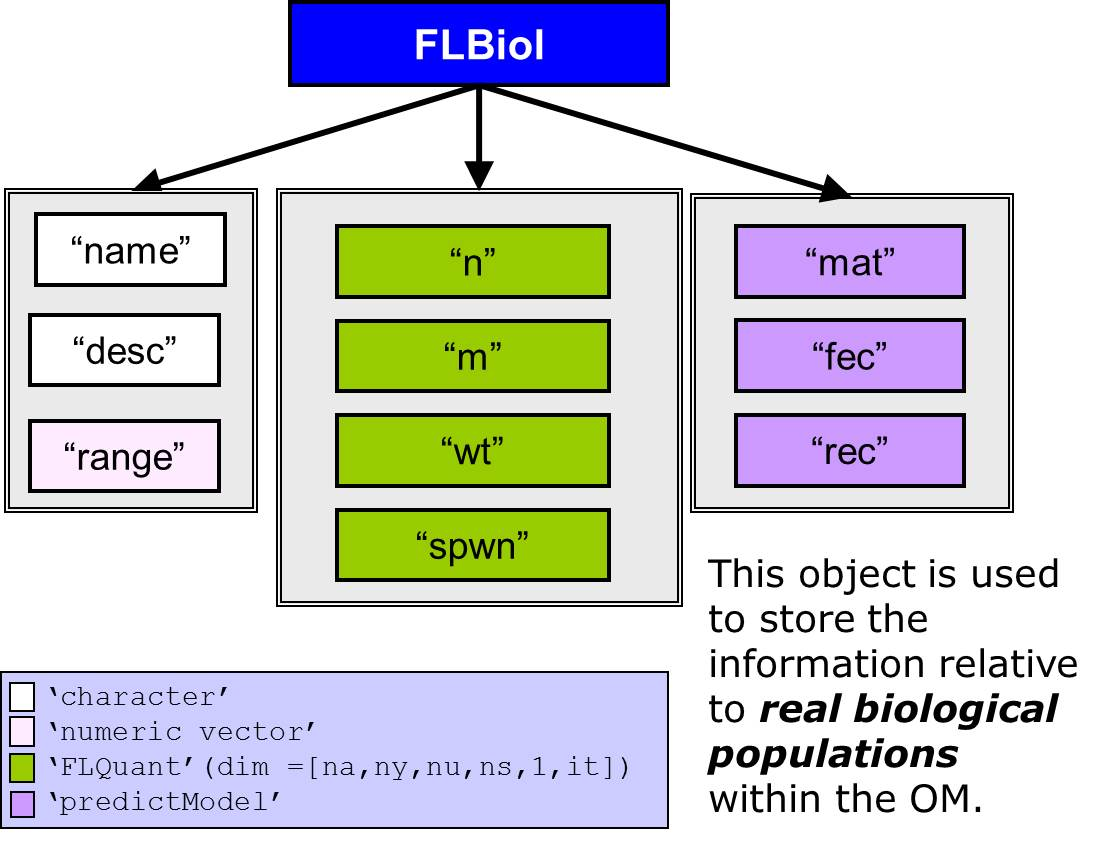
\includegraphics[width= 0.9\textwidth]{FLBiol}
   \caption{FLBiol object}
   \label{fig:FLBiol}
\end{figure}


% FLFleetExt
\begin{figure}[!h]
  \centering
    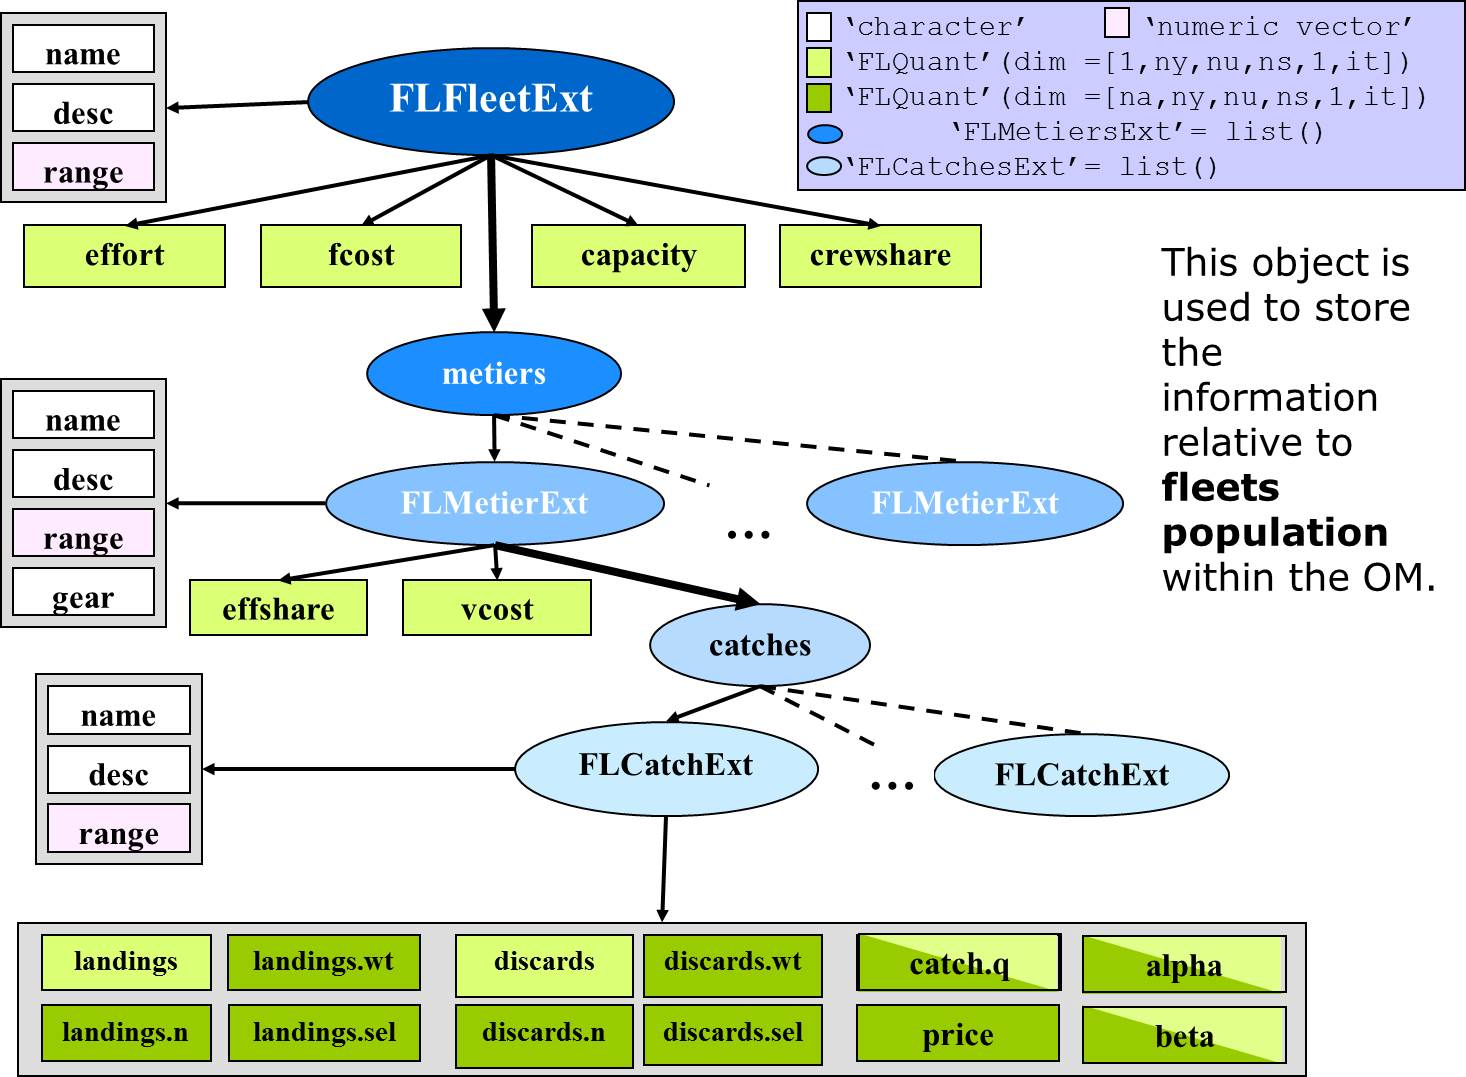
\includegraphics[width= 0.9\textwidth]{FLFleetExt}
  \caption{FLFleetExt object}
  \label{fig:FLFleetExt}
\end{figure}

% FLSRsim
\begin{figure}[!h]
  \centering
    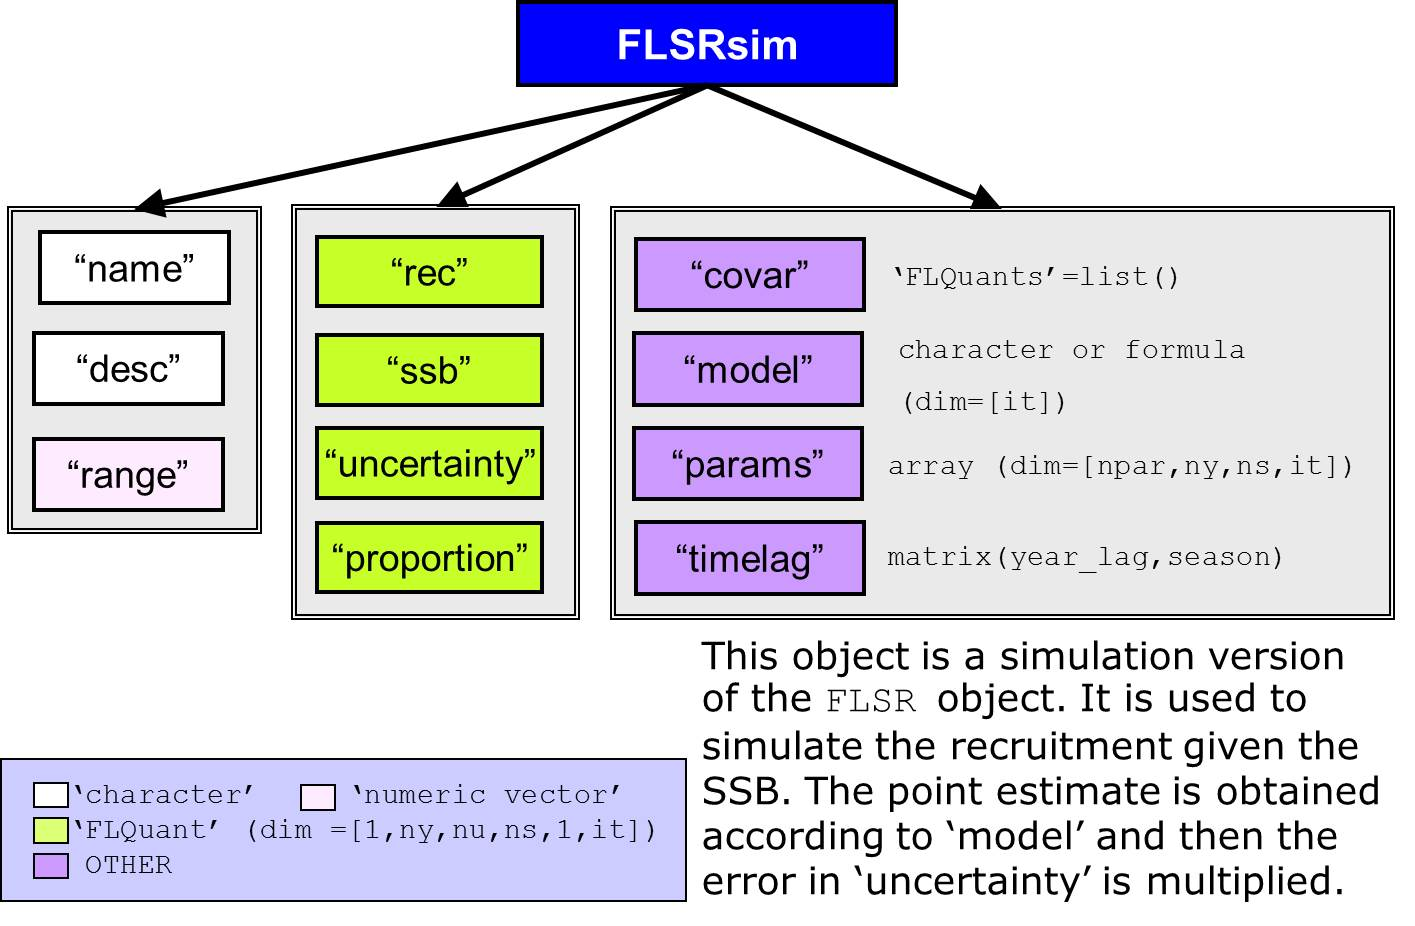
\includegraphics[width= 0.9\textwidth]{FLSRsim}
  \caption{FLSRsim object}
  \label{fig:FLSRsim}
\end{figure}

% FLBDsim
\begin{figure}[!h]
  \centering
    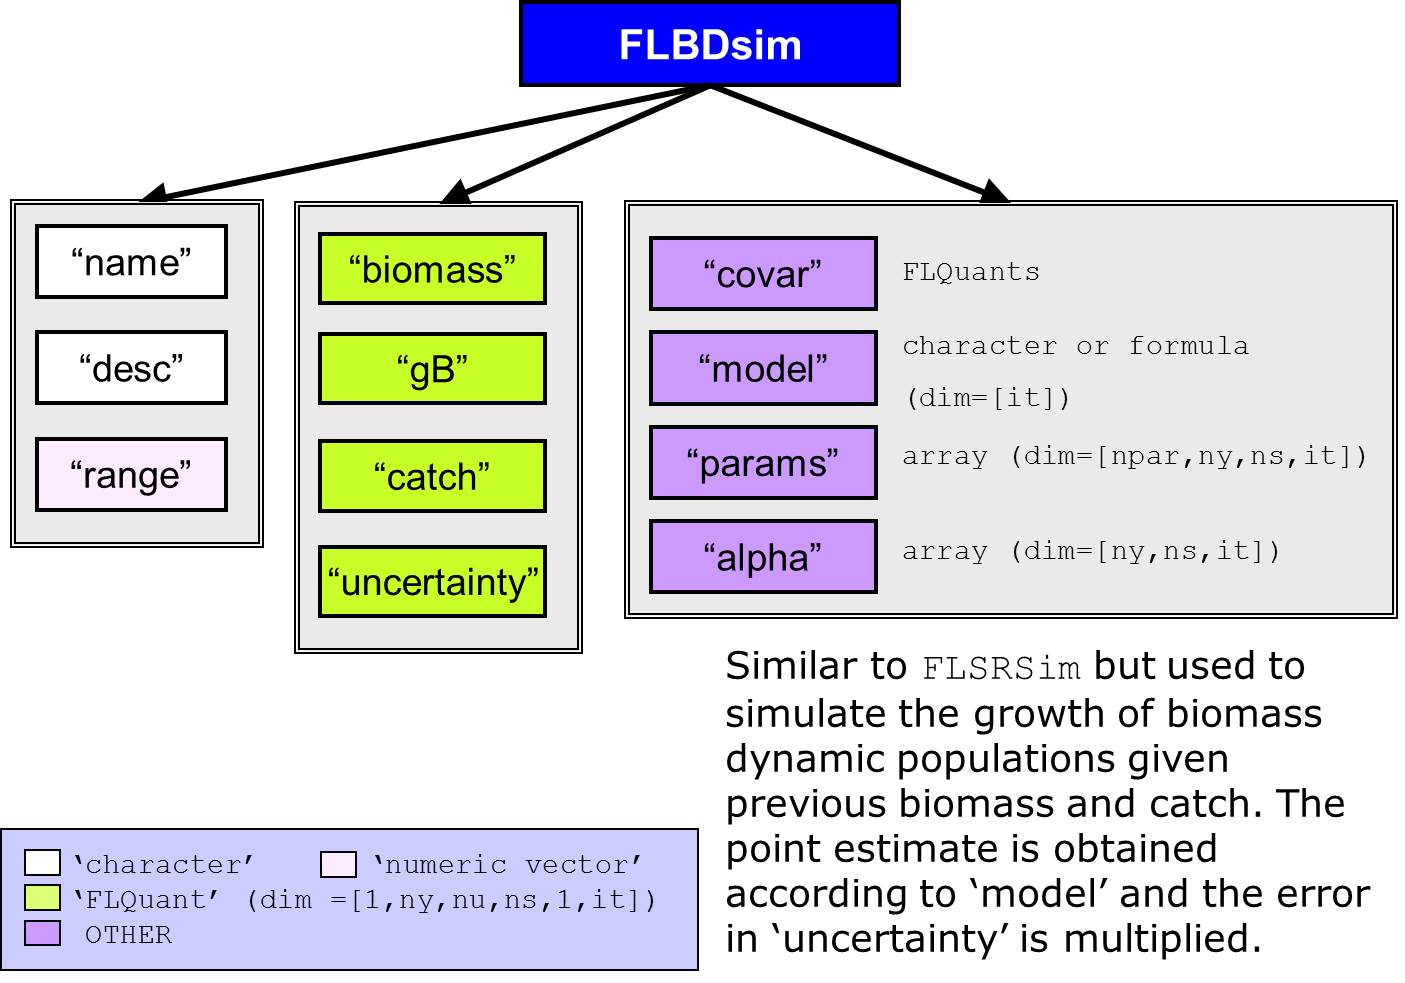
\includegraphics[width= 0.9\textwidth]{FLBDsim}
  \caption{FLBDsim object}
  \label{fig:FLBDsim}
\end{figure}

% FLIndex
\begin{figure}[!h]
  \centering
    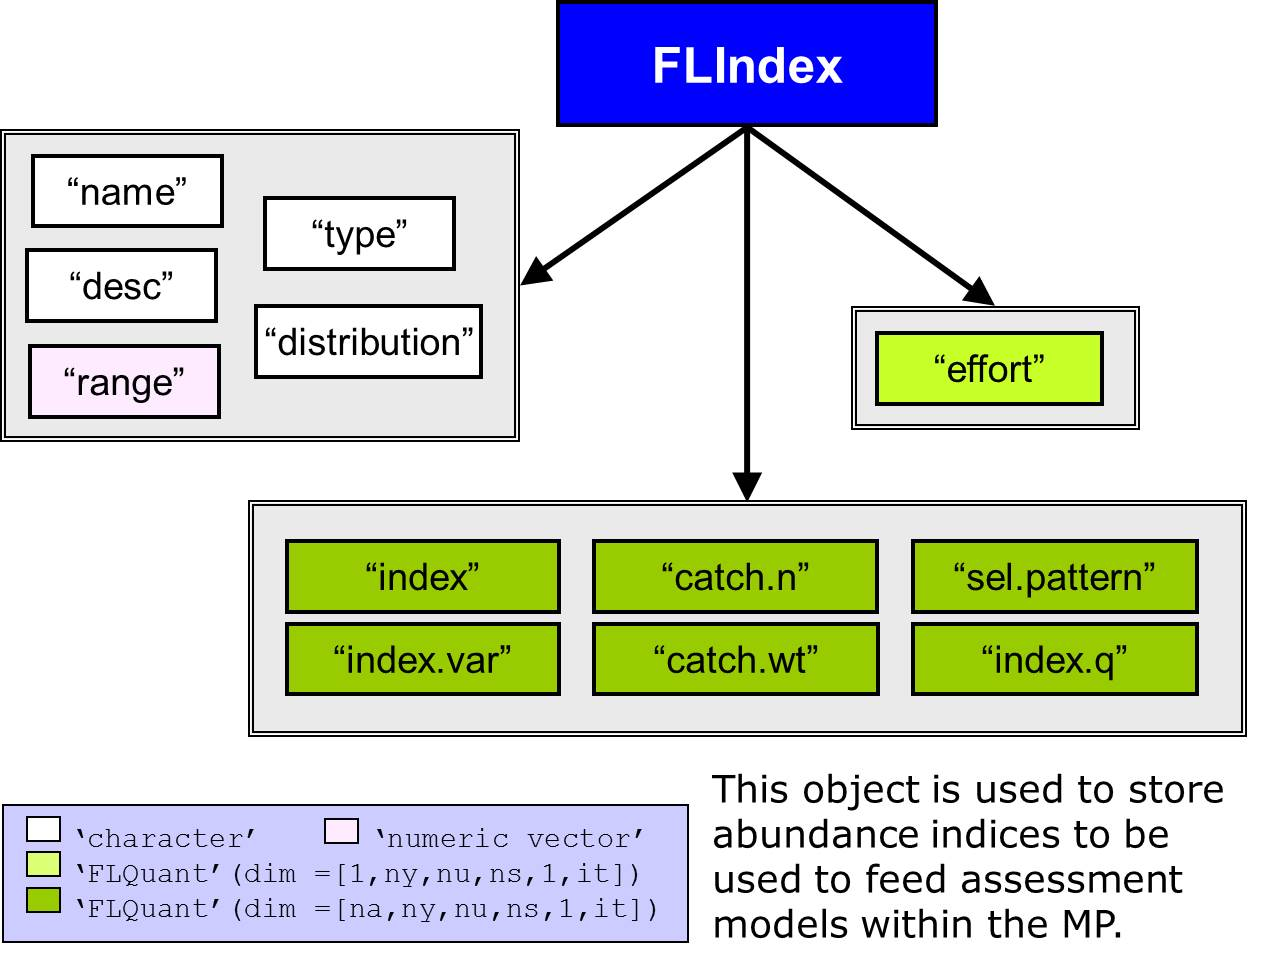
\includegraphics[width= 0.9\textwidth]{FLIndex}
  \caption{FLIndex object}
  \label{fig:FLIndex}
\end{figure}

% FLStock
\begin{figure}[!h]
  \centering
    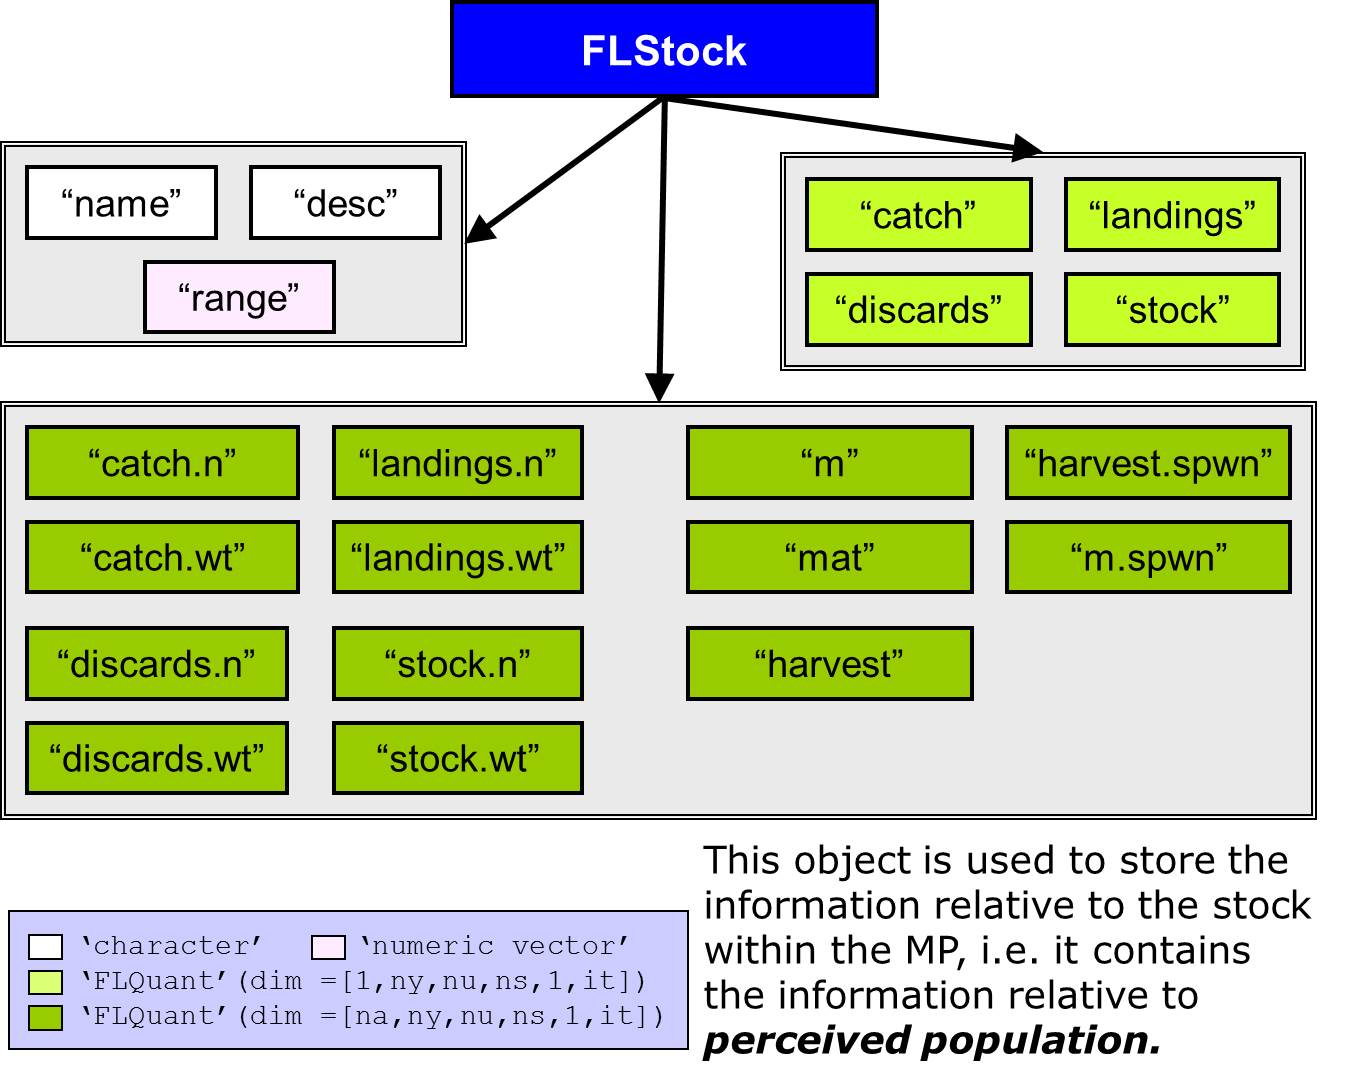
\includegraphics[width= 0.9\textwidth]{FLStock}
  \caption{FLStock object}
  \label{fig:FLStock}
\end{figure}
%\appendix

\begin{landscape}

\section{Graphical representation of control objects} \label{sec:CtrlObj_tab}

\setcounter{figure}{0} 
\setcounter{table}{0}

%TABLE 1
\begin{table}[!ht]

  %\begin{center}
  \centering
  \begin{footnotesize}
    
    \caption{Description of all the optional arguments for \texttt{main.ctrl} object (of class list).
    The arguments with \textsuperscript{*} are compulsory arguments.}
    
    \label{tb:A3.table1}
    
    \begin{threeparttable}
    
      \begin{tabular}{lllll} %{c|c}
        \hline 
        Argument & class & Dimension & Values & Required for \\
        \hline
        sim.years\textsuperscript{*} & numeric vector & 2 (initial,final) & any in year range & \\
        \hline
      \end{tabular}
      
    \end{threeparttable}
  \end{footnotesize}
  %\end{center}

\end{table}


%TABLE 2
\begin{table}[!ht]

  %\begin{center}
  \centering
  \begin{footnotesize}
    
    \caption{Description of all the optional arguments for \texttt{biols.ctrl} object (of class list).
    The arguments with \textsuperscript{*} are compulsory arguments.}
    
    \label{tb:A3.table2}
    
    \begin{threeparttable}
    
      \begin{tabular}{lllll} %{c|c}
        \hline 
        Argument & class & Dimension & Values & Required for \\
        \hline
        {[[st]]}\$growth.model\textsuperscript{*} & character & 1 & \texttt{'fixedPopulation'},\texttt{'ASPG'} & \texttt{BDPG}  \\
        \hline
      \end{tabular}
      
    \end{threeparttable}
  \end{footnotesize}
  %\end{center}

\end{table}


%TABLE 3
\begin{table}[!ht]

  %\begin{center}
  \centering
  \begin{footnotesize}
    
    \caption{Description of all the optional arguments for \texttt{fleets.ctrl} object (of class list).
    In the table we assume that \texttt{stk} is the name of the stock and \texttt{fl} the name of the fleet.
    The arguments with \textsuperscript{*} are compulsory arguments.}
    
    \label{tb:A3.table3}
    
    \begin{threeparttable}
    
      \begin{tabular}{lllll} %{c|c}
        \hline 
        Argument & class & Dimension & Values & Required for \\
        \hline
        catch.treshold & FLQuant & [nst,ny,1,ns,1,ni] & Proportions in [0,1] range & \texttt{SMFB}, \texttt{SSFB} \\
        seasonal.share[[st]]              & FLQuant & [nst,ny,1,ns,1,ni] & Proportionsin [0,1] (sum along seasons = 1) & 
          \texttt{SMFB}, \texttt{SSFB} \\
        {[[fl]]}\$effort.model\textsuperscript{*} & character & 1 & \texttt{'fixedEffort'},\texttt{'SMFB'},\texttt{'SSFB'},  &	\\
         &  &  & \texttt{'MaxProfit'}, \texttt{'MaxProfitSeq'}  &	\\
        {[[fl]]}\$restriction & character & 1 & \texttt{'catch'},\texttt{'landings'} & \texttt{SMFB}, \texttt{SSFB}  \\
        {[[fl]]}\$effort.rest & character & 1 & \texttt{'max'},\texttt{'min'},\texttt{'mean'},\texttt{'prev'},\texttt{stock.name} & 
          \texttt{SMFB}, \texttt{SSFB}  \\
        {[[fl]]}\$effectiveDay.perc & FLQuant & [1,ny,1,ns,1,ni]  & Proportions in [0,1] & \texttt{SSFB} \\
        {[[fl]]}\$effort.realloc & character & 1 & \texttt{NULL},\texttt{'curr.eff'} & \texttt{SSFB} \\
        {[[fl]]}\$stk.cnst & character & 1 & \texttt{stock.name} & \texttt{MaxProfit} \\
        {[[fl]]}\$capital.model\textsuperscript{*} & character & 1 & \texttt{'fixedCapital'},\texttt{'SCD'} & \\
        {[[fl]]}[[st]]\$catch.model\textsuperscript{*} & character & 1 & \texttt{'cobbDouglasBio'},\texttt{'cobbDouglasAge'}, &  \\
         &  &  & \texttt{'seasonshare'}  &	\\
        {[[fl]]}[[st]]\$catch.dependence\textsuperscript{1} & character & nfl & \texttt{fleet.name} \ & \texttt{seasonShare} \\
        {[[fl]]}[[st]]\$TAC.OS.model & character & 1 & \texttt{'TAC.OS.triangCond'} & \texttt{SMFB}, \texttt{MaxProfit} \\
        {[[fl]]}[[st]]\$TAC.OS.triangCond.params & named numeric vector & 3 (min,max,mode) &  & \texttt{SMFB}, \texttt{MaxProfit} \\
        {[[fl]]}[[st]]\$discard.TAC.OS & logical & 1 & \texttt{'TRUE'} (TAC overshoot is discarded), \\
         &  &  & \texttt{'FALSE'} (TAC overshoot is included in landings) & \texttt{SMFB}, \texttt{MaxProfit} \\
        {[[fl]]}[[st]]\$price.model\textsuperscript{*} & character & 1 & \texttt{'fixedPrice'}, \texttt{'elasticPrice'} &  \\
        {[[fl]]}[[st]]\$pd.els & numeric array & [na,ns,ni] &  &  \texttt{elasticPrice} \\
        {[[fl]]}[[st]]\$pd.La0 & numeric array & [na,ns,ni] &  &  \texttt{elasticPrice} \\
        {[[fl]]}[[st]]\$pd.Pa0 & numeric array & [na,ns,ni] &  &  \texttt{elasticPrice} \\
        {[[fl]]}[[st]]\$pd.total & logical & 1 & \texttt{'TRUE'} (if depending on total catch), \texttt{'FALSE'} & 
          \texttt{elasticPrice} \\
        \hline
      \end{tabular}
      
      \begin{tablenotes}
        % \small
        \item nst: number of stocks
        \item nfl: number of fleets
        \item na: number of age clases
        \item ny: number of years
        \item ns: number of seasons
        \item ni: number of iterations
        \item \textsuperscript{1}If defined, takes the same seasonal share as the one of fleet \texttt{fleet.name}.
      \end{tablenotes}
      
    \end{threeparttable}
  \end{footnotesize}
  %\end{center}

\end{table}	


%TABLE 4
\begin{table}[!ht]

  %\begin{center}
  \centering
  \begin{footnotesize}

    \caption{Description of all the optional arguments for \texttt{covars.ctrl} object (of class list).
    In the table we assume that \texttt{cv} is the name of the covariate.
    The arguments with \textsuperscript{*} are compulsory arguments.}
    
    \label{tb:A3.table4}

    \begin{threeparttable}

      \begin{tabular}{lllll} %{c|c}
        \hline
        Argument & class & Dimension & Values & Required for \\
        \hline
        {[[cv]]}\$process.model\textsuperscript{*} & character & 1 & \texttt{'fixedCovar'},\texttt{'ssb.get'}  &	\\
        {[[cv]]}\$ssb.stock & character & 1 & \texttt{stock.name} &	\texttt{ssb.get} \\
        {[[cv]]}\$spwn.season & numeric & 1 & \texttt{season} &	\texttt{ssb.get} \\
        {[[cv]]}\$sr.covar & character & 1 & \texttt{stock.name} &	\texttt{ssb.get} \\
        \hline
      \end{tabular}

    \end{threeparttable}
  \end{footnotesize}
  %\end{center}

\end{table}


%TABLE 5
\begin{table}[!ht]

  %\begin{center}
  \centering
  \begin{footnotesize}

    \caption{Description of all the optional arguments for \texttt{obs.ctrl} object (of class list).
    In the table we assume that \texttt{stk} is the name of the stock and \texttt{id} the name of the index.
    The arguments with \textsuperscript{*} are compulsory arguments.}
    
    \label{tb:A3.table5}

    +++++ SONIA: no descrito nada de esto en el texto, necesitariamos extender informacion?

    \begin{threeparttable}

      \begin{tabular}{lllll} %{c|c}
        \hline
        Argument & class & Dimension & Values & Required for \\
        \hline
        % {[[st]]}\$obs.curryr\textsuperscript{1} & logical & 1 & \texttt{'TRUE'} (if current year also observed), \texttt{'FALSE'} (only up to y-1) &  \\
        {[[st]]}\$stkObs\$stkObs.model\textsuperscript{*} & character & 1 & \texttt{'NoObsStock'},\texttt{'perfectObs'},
          \texttt{'age2ageDat'},\texttt{'age2agePop'}, &  \\
         &  &  & \texttt{'age2bioDat'},\texttt{'age2bioPop'},\texttt{'bio2bioDat'},\texttt{'bio2bioPop'} &  \\
        {[[st]]}\$stkObs\$TAC.ovrsht & array & [1,ny] & In percentage per unit & \texttt{age2ageDat},\texttt{age2bioDat},\texttt{bio2bioDat} \\
        {[[st]]}\$stkObs\$ages.error\textsuperscript{2} & array & [na,na,ny,ni] & In percentage per unit & \texttt{age2ageDat},\texttt{age2agePop} \\
        {[[st]]}\$stkObs\$nmort.error & FLQuant & [na,ny,1,1,1,ni] & any & \texttt{age2ageDat} \\
        {[[st]]}\$stkObs\$mat.error & FLQuant & [na,ny,1,1,1,ni] & any & \texttt{age2ageDat} \\
        {[[st]]}\$stkObs\$stk.nage.error & FLQuant & [na,ny,1,1,1,ni] & any & \texttt{age2agePop} \\
        {[[st]]}\$stkObs\$stk.wgt.error & FLQuant & [na,ny,1,1,1,ni] & any & \texttt{age2agePop} \\
        {[[st]]}\$stkObs\$stk.bio.error & FLQuant & [1,ny,1,1,1,ni] & any & \texttt{age2bioPop},\texttt{bio2bioDat},\texttt{bio2bioPop} \\
        {[[st]]}\$stkObs\$land.nage.error & FLQuant & [na,ny,1,1,1,ni] & any & \texttt{age2ageDat} \\
        {[[st]]}\$stkObs\$land.wgt.error & FLQuant & [na,ny,1,1,1,ni] & any & \texttt{age2ageDat}\\
        {[[st]]}\$stkObs\$land.bio.error & FLQuant & [1,ny,1,1,1,ni] & any & \texttt{age2bioDat},\texttt{bio2bioDat},\texttt{bio2bioPop} \\
        {[[st]]}\$stkObs\$disc.nage.error & FLQuant & [na,ny,1,1,1,ni] & any & \texttt{age2ageDat} \\
        {[[st]]}\$stkObs\$disc.wgt.error & FLQuant & [na,ny,1,1,1,ni] & any & \texttt{age2ageDat} \\
        {[[st]]}\$stkObs\$disc.bio.error & FLQuant & [1,ny,1,1,1,ni] & any & \texttt{age2bioDat},\texttt{bio2bioDat},\texttt{bio2bioPop} \\
        {[[st]]}\$indObs[[id]]\$indObs.model\textsuperscript{*} & character & 1 & \texttt{'NoObsIndex'},\texttt{'NoObservation'},\texttt{'ageInd'},
          \texttt{'bioInd'} &  \\
        % +++ SONIA pendiente de incluir: ,\texttt{'ssbInd'},\texttt{'cbbmInd'} for ANE
        % {[[st]]}\$indObs[[id]]$sInd & numeric & 1 & \texttt{season.name} (season in which index is observed) & \texttt{'ssbInd'} \\
        % {[[st]]}\$indObs[[id]]$wageIni & matrix & [2,ni] & weight at age for each age class (age1,age2plus) & \texttt{'ssbInd'} \\
        \hline
      \end{tabular}

      \begin{tablenotes}
        % \small
        \item na: number of age clases
        \item ny: number of years
        \item ni: number of iterations
        % \item \textsuperscript{1}If \texttt{advice.ctrl[[st]]\$ass.curryr=TRUE} then this value is authomatically set to \texttt{TRUE}.
        \item \textsuperscript{2}For each year and iteration, there is a square matrix
          whose column elements quantify the probability that a fish of age $a$ is classified as having any age between
          $min(age)$ and $max(age)$.
      \end{tablenotes}

    \end{threeparttable}
  \end{footnotesize}
  %\end{center}

\end{table}
	

%TABLE 6
\begin{table}[!ht]

  %\begin{center}
  \centering
  \begin{footnotesize}

    \caption{Description of all the optional arguments for \texttt{assess.ctrl} object (of class list).
    In the table we assume that \texttt{stk} is the name of the stock.
    The arguments with \textsuperscript{*} are compulsory arguments.}
    
    \label{tb:A3.table6}

    +++++ SONIA: no descrito en el texto, necesitariamos extender informacion?

    \begin{threeparttable}

      \begin{tabular}{lllll} %{c|c}
        \hline
        Argument & class & Dimension & Values & Required for \\
        \hline
        {[[st]]}\$assess.model\textsuperscript{*} & character & 1 & \texttt{'NoAssessment'},\texttt{'FLXSAnew'},... &  \\
        % +++++ SONIA: para cuando se introduzcan los cambios de estacionalidad (ANE)
        % {[[st]]}\$assess.curryr\textsuperscript{1} & logical & 1 & \texttt{'TRUE'} (for getting also estimates for assessment year), & 
        %   \texttt{assess.ctrl[[st]]\$assess.model != 'NoAssessment'}\\
        %  &  &  & \texttt{'FALSE'} (default) &  \\
        {[[st]]}\$control & control object &  & Depends on the selected assessment model & \texttt{assess.ctrl[[st]]\$assess.model} \\
         &  &  & (e.g. \texttt{FLXSA.control()} for XSA assessment) &  \\
        \hline
      \end{tabular}

     \end{threeparttable}
  \end{footnotesize}
  %\end{center}

\end{table}
	

%TABLE 7
\begin{table}[!ht]

  %\begin{center}
  \centering
  \begin{footnotesize}

    \caption{Description of all the optional arguments for \texttt{advice.ctrl} object (of class list).
    In the table we assume that \texttt{stk} is the name of the stock and \texttt{id} the name of the index.
    The arguments with \textsuperscript{*} are compulsory arguments.}
    
    \label{tb:A3.table7}

    \begin{threeparttable}

      \begin{tabular}{lllll} %{c|c}
        \hline
        Argument & class & Dimension & Values & Required for \\
        \hline
        {[[st]]}\$HCR.model\textsuperscript{*} & character & 1 & \texttt{'fixedAdvice'},\texttt{'annualTAC'},\texttt{'IcesHCR'},\texttt{'FroeseHCR'}, &  \\
         &  &  & \texttt{'annexIVHCR'},\texttt{'ghlHCR'},\texttt{'aneHCRE'},\texttt{'neaMAC\_ltmp'}, &  \\
         &  &  & \texttt{'F2CatchHCR'},\texttt{'little2011HCR'},\texttt{'pidHCR'},\texttt{'pidHCRtarg'}, &  \\
         &  &  & \texttt{'MAPHCR'},\texttt{'CFPMSYHCR'},\texttt{'MultiStockHCR'} &  \\
         {[[st]]}\$AdvCatch & logical & 1 & \texttt{'TRUE'} (TAC in terms of catch), & \texttt{annualTAC}, \texttt{IcesHCR}, \texttt{CFPMSYHCR}, \\
         &  &  & \texttt{'FALSE'} (TAC in terms of landings) & \texttt{MAPHCR}, \texttt{F2CatchHCR} \\
        {[[st]]}\$nyears & numeric & 1 & season.name & \texttt{annualTAC}, \texttt{IcesHCR}, \texttt{F2CatchHCR},  \\
         &  &  &  & \texttt{MultiStockHCR} \\
        {[[st]]}\$wts.nyears & numeric & 1 & season.name & \texttt{annualTAC}, \texttt{IcesHCR}, \texttt{MAPHCR}, \\
         &  &  &  & \texttt{CFPMSYHCR}, \texttt{F2CatchHCR}, \texttt{MultiStockHCR} \\
        {[[st]]}\$fbar.nyears & numeric & 1 & season.name & \texttt{annualTAC}, \texttt{IcesHCR}, \texttt{MAPHCR}, \\
         &  &  &  & \texttt{CFPMSYHCR}, \texttt{F2CatchHCR}, \texttt{MultiStockHCR} \\
        {[[st]]}\$f.rescale & logical & 1 & \texttt{'TRUE'} (???), \texttt{'FALSE'} & \texttt{annualTAC}, \texttt{IcesHCR}, \texttt{MAPHCR}, \\
         &  &  &  & \texttt{CFPMSYHCR}, \texttt{F2CatchHCR}, \texttt{MultiStockHCR} \\
        {[[st]]}\$disc.nyears & numeric & 1 &  & \texttt{annualTAC}, \texttt{CFPMSYHCR}  \\
        {[[st]]}\$fwd.control & fwdBDcontrol &  &  & \texttt{annualTAC}  \\
        {[[st]]}\$sr$model & character &  1 & SR model name  & \texttt{annualTAC}, \texttt{IcesHCR}, \texttt{MAPHCR}, \\
         &  &  &  & \texttt{F2CatchHCR}, \texttt{MultiStockHCR} \\
        {[[st]]}\$sr$params\textsuperscript{1} & FLPar & [npar,ni]  &  & \texttt{annualTAC}, \texttt{IcesHCR}, \texttt{MAPHCR}, \\
         &  &  &  & \texttt{CFPMSYHCR}, \texttt{F2CatchHCR}, \texttt{MultiStockHCR} \\
         {[[st]]}\$sr$years\textsuperscript{1} & named numeric vector & 2 (y.rm, num.years) &  & \texttt{annualTAC}, \texttt{IcesHCR}, \texttt{MAPHCR}, \\
         &  &  &  & \texttt{CFPMSYHCR}, \texttt{F2CatchHCR}, \texttt{MultiStockHCR} \\
        {[[st]]}\$growth.years\textsuperscript{2} & named numeric vector & 2 (y.rm, num.years) &  & \texttt{annualTAC}, \texttt{IcesHCR}, \texttt{CFPMSYHCR}, \\
         &  &  &  & \texttt{F2CatchHCR}, \texttt{MultiStockHCR} \\
        {[[st]]}\$ref.pts & matrix & [nrp,ni] &  & \texttt{IcesHCR}, \texttt{FroeseHCR}, \texttt{annexIVHCR}, \\
         &  &  &  & \texttt{ghlHCR}, \texttt{MAPHCR}, \texttt{CFPMSYHCR}, \\
         &  &  &  & \texttt{F2CatchHCR}, \texttt{little2011HCR}, \texttt{pidHCR}, \\
         &  &  &  & \texttt{pidHCRtarg}, \texttt{MultiStockHCR} \\
        {[[st]]}\$intermediate.year & character & 1 & \texttt{'Fsq'} or any &  \texttt{IcesHCR}, \texttt{neaMAC\_ltmp}, \texttt{F2CatchHCR}, \\
         &  &  &  & \texttt{MultiStockHCR} \\
        {[[st]]}\$index & character & 1 & index.name & \texttt{annexIVHCR}, \texttt{little2011HCR}, \texttt{pidHCR}, \\
         &  &  &  & \texttt{pidHCRtarg} \\
        {[[st]]}\$type & numeric & 1 & \texttt{2} or \texttt{4} & \texttt{annexIVHCR}  \\
        {[[st]]}\$N & numeric & 1 &  & \texttt{MAPHCR},\texttt{CFPMSYHCR} \\
        {[[st]]}\$stocksInHCR & vector & any &  names of the stocks to be taken into account & \texttt{MultiStockHCR}  \\
        % +++ SONIA pendiente de incluir: changes for ANE
        % {[[st]]}\$ass.year & character & any & year.names for wich assessment is required & \texttt{???} \\
        % {[[st]]}\$ass.curryr & logical & 1 & \texttt{'TRUE'} (if estimates for assessment year needed to give advice), & \texttt{???} \\
        %  &  &  & \texttt{'FALSE'} (default) &  \\
        % {[[st]]}\$ass.season & numeric & 1 & season.name & \texttt{???} \\
        % 
        % {[[st]]}\$TACs1.perc & numeric & 1 & percentage of TAC assumed to be taken in the 1st semester & \texttt{aneHCRs} \\
        % {[[st]]}\$tsurv & numeric & 1 & time period of the survey & \texttt{aneHCRs} \\
        % {[[st]]}\$cbbm.params$G & FLQuant & [2,ny,1,1,1,ni]  &  & \texttt{aneHCRs} \\
        % {[[st]]}\$cbbm.params$M & FLQuant & [2,ny,1,1,1,ni]  &  & \texttt{aneHCRs} \\
        % {[[st]]}\$cbbm.params$S & FLQuant & [2,ny,1,1,1,ni]  &  & \texttt{aneHCRs} \\
        \hline
      \end{tabular}

      \begin{tablenotes}
        % \small
        \item npar: number of parameters in the SR model selected for stock \texttt{st}.
        \item nrp: number of reference points required for the HCR selected for stock \texttt{st}.
        \item ny: number of years
        \item ni: number of iterations
        \item \textsuperscript{1}Optional argument for the function.
        \item \textsuperscript{2}Used only for stocks aggregated in biomass.
      \end{tablenotes}

    \end{threeparttable}
  \end{footnotesize}
  %\end{center}

\end{table}        



\end{landscape}


%\appendix

\begin{landscape}

\section{Smart conditioning - function's arguments description} \label{sec:SmartCond_tab}

\setcounter{figure}{0} 
\setcounter{table}{0}

% \subsection{Tables}

%TABLE 1
\begin{table}[!ht]

  %\begin{center}
  \centering
  \begin{footnotesize}
    
    \caption{Description of the arguments of the function \texttt{create.biols.data}. 
      In the table we assume that \texttt{stk} is the name of the stock. All the arguments are required.}
    
    \label{tb:A4.table1}
    
    \begin{threeparttable}
    
      \begin{tabular}{lllll} %{c|c}
        \hline 
        Argument & & class & Dimension & Definition\\
        \hline
        yrs & & vector & 3 &	c( first.yr, proj.yr, last.yr)\\
          & first.yr & numeric & 1 & First year of simulation\\
          & proj.yr  & numeric & 1 & First year of projection\\
          & last.yr  & numeric & 1 & Last year of projection\\
        ni & & numeric &	1 &	Number of iterations\\
        ns & & numeric &	1 &	Number of seasons\\
        stks.data & &	list & number of stocks &	List with the name of the stocks and the following elements:\\
          & stk.unit    &	numeric &	1 &	Number of units\\
          & stk.age.min &	numeric &	1 &	Minimum age\\ 
          & stk.age.max &	numeric &	1 &	Maximum age\\
          & stk\_n.flq    &	FLQuant &	[na,ny(hist),1/nu(stock),1/ns,1/ni] &	Abundance in numbers at age\\
          & stk\_wt.flq   &	FLQuant &	[na,ny(hist),1/nu(stock),1/ns,1/ni] &	Weight at age\\
          & stk\_m.flq    &	FLQuant &	[na,ny(hist),1/nu(stock),1/ns,1/ni] &	Natural mortality mortality rate\\
          & stk\_fec.flq  &	FLQuant &	[na,ny(hist),1/nu(stock),1/ns,1/ni] &	Fecundity\\
          & stk\_mat.flq  &	FLQuant &	[na,ny(hist),1/nu(stock),1/ns,1/ni] &	Percentage of mature individuals\\
          & stk\_spwn.flq &	FLQuant &	[na,ny(hist),1/nu(stock),1/ns,1/ni] &	Proportion of time step at spawning\\
          & stk\_range.min       &	numeric &	1 &	Minimum age\\
          & stk\_range.max       &	numeric &	1 &	Maximum age\\
          & stk\_range.plusgroup &	numeric &	1 &	Plusgroup age\\
          & stk\_range.minyear   &	numeric &	1 &	Minimum year\\
          & stk\_range.maxyear   &	numeric &	1 &	Maximum year\\
          & stk\_range.minfbar   &	numeric &	1 &	Minimum age for calculating average fishing mortality\\
          & stk\_range.maxfbar   &	numeric &	1 &	Maximum age for calculating average fishing mortality \\
          & stk\_biol.proj.avg.yrs &	vector &	any &	Historic years to calculate averages (in spwn, fec, m and wt)\\
          &  &	&	&	for the projection period\\
        \hline
      \end{tabular}
      
      \begin{tablenotes}
        % \small
        \item na: number of age (from min.age to max.age)
        \item ny(hist): number of historic years (from first.yr to proj.yr-1)
        \item 1/nu(stock): 1 or number of units of the stock
        \item 1/ns: 1 or number of seasons
        \item 1/ni:  1 or number of iterations
      \end{tablenotes}
      
    \end{threeparttable}
  \end{footnotesize}
  %\end{center}

\end{table}			

	

%TABLE 2
\begin{table}[!ht]

  %\begin{center}
  \centering
  \begin{footnotesize}
    
    \caption{Description of the arguments of the function \texttt{create.SRs.data}. 
      In the table we assume that \texttt{stk} is the name of the stock. 
      The arguments with superscript \textsuperscript{*} are optional arguments.}
      
    \label{tb:A4.table2}
    
    \begin{threeparttable}
    
      \begin{tabular}{lllll} %{c|c}
        \hline 
        Argument & & class & Dimension & Definition\\
        \hline
        yrs & & vector & 3 &	c( first.yr, proj.yr, last.yr)\\
          & first.yr & numeric & 1 & First year of simulation\\
          & proj.yr  & numeric & 1 & First year of projection\\
          & last.yr  & numeric & 1 & Last year of projection\\
        ni & & numeric &	1 &	Number of iterations\\
        ns & & numeric &	1 &	Number of seasons\\
        stks.data & &	list & number of stocks &	List with the name of the stocks and the following elements:\\
          & stk.unit          &	numeric &	1 &	Number of units\\
          & stk.age           &	numeric &	1 &	Number of age classes\\
          & stk\_sr.model     & character &	1 &	Name of the SR model\\ 
          & stk\_params.n     &	vector &	1  &	Number of parameters\\ 
          & stk\_params.name  &	vector &	stk\_params.n &	Name of the parameters\\
          & stk\_params.array &	array &	[stk\_params.n,ny,ns,1/ni] &	Parameter values\\
          & stk\_rec.flq  &	FLQuant &	[1,ny(hist),1/nu(stock),1/ns,1/ni] &	Recruitment values\\
          & stk\_ssb.flq  &	FLQuant &	[1,ny(hist),1/nu(stock),1/ns,1/ni] &	Spawning stock values\\
          & stk\_uncertainty.flq\textsuperscript{*} & FLQuant & [1,ny,1/nu(stock),1/ns,1/ni] & Uncertainty\\
          & stk\_proportion.flq  &	FLQuant &	[1,ny,1/nu(stock),1/ns,1/ni] &	Recruitment distribution in each time step. For details see \texttt{FLSRsim}\\
          & stk\_prop.avg.yrs &	vector & any & Historical years to calculate the proportion average\\
          & stk\_timelag.matrix  &	matrix &	(2,ns) &	Timelag between the spawning an recruitment (time.lag.yr, time.lag.ns)\\
          & & & & For details see \texttt{FLSRsim}\\
          & stk\_range.min       &	numeric &	1 &	Minimum age\\
          & stk\_range.max       &	numeric &	1 &	Maximum age\\
          & stk\_range.plusgroup &	numeric &	1 &	Plusgroup age\\
          & stk\_range.minyear   &	numeric &	1 &	Minimum year\\
          % & stk\_range.maxyear   &	numeric &	1 &	Maximum year\\
        \hline
      \end{tabular}
      
      \begin{tablenotes}
        % \small
        \item na: number of age (from min.age to max.age)
        \item ny(hist): number of historic years (from first.yr to proj.yr-1)
        \item ny: number of years (from first.yr to last.yr)
        \item 1/nu(stock): 1 or number of units of the stock
        \item 1/ns: 1 or number of seasons
        \item 1/ni: 1 or number of iterations
        \item ns: number of seasons
      \end{tablenotes}
      
    \end{threeparttable}
  \end{footnotesize}
  %\end{center}

\end{table}			



%TABLE 3
\begin{table}[!ht]

  %\begin{center}
  \centering
  \begin{footnotesize}
    
    \caption{Description of the arguments of the function \texttt{create.BDs.data}. 
      In the table we assume that \texttt{stk} is the name of the stock. 
      The arguments with \textsuperscript{*} are optional arguments.}
    
    \label{tb:A4.table3}
    
    \begin{threeparttable}
    
      \begin{tabular}{lllll} %{c|c}
        \hline 
        Argument & & class & Dimension & Definition\\
        \hline
        yrs & & vector & 3 &	c( first.yr, proj.yr, last.yr)\\
          & first.yr & numeric & 1 & First year of simulation\\
          & proj.yr  & numeric & 1 & First year of projection\\
          & last.yr  & numeric & 1 & Last year of projection\\
        ni & & numeric &	1 &	Number of iterations\\
        ns & & numeric &	1 &	Number of seasons\\
        stks.data & &	list & number of stocks &	List with the name of the stocks and the following elements:\\
          & stk.unit          &	numeric &	1 &	Number of units\\
          & stk\_bd.model     & character &	1 &	Name of the BD model\\ 
          & stk\_params.name  &	vector &	np &	Name of the parameters\\ 
          & stk\_params.array &	vector &	np &	Parameter values\\
          & stk\_biomass.flq  &	FLQuant &	[1,ny(hist),1/nu(stock),1/ns,1/ni] &	Biomass values\\
          & stk\_catch.flq    &	FLQuant &	[1,ny(hist),1/nu(stock),1/ns,1/ni] &	Catch values\\
          & stk\_range.min       &	numeric &	1 &	Minimum age\\
          & stk\_range.max       &	numeric &	1 &	Maximum age\\
          & stk\_range.plusgroup &	numeric &	1 &	Plusgroup age\\
          & stk\_range.minyear   &	numeric &	1 &	Minimum year\\
          % & stk\_range.maxyear   &	numeric &	1 &	Maximum year\\
          & stk\_alpha        &	numeric &	1 &	Maximum variability of carrying capacity\\
          & stk\_gB.flq\textsuperscript{*} & FLQuant & [1,ny(hist),1/nu(stock),1/ns,1/ni] & Surplus production values\\
          & stk\_uncertainty.flq\textsuperscript{*} & FLQuant & [1,ny,1/nu(stock),1/ns,1/ni] & Uncertainty\\
        \hline
      \end{tabular}
      
      \begin{tablenotes}
        % \small
        \item na: number of age (from min.age to max.age)
        \item ny(hist): number of historic years (from first.yr to proj.yr-1)
        \item ny: number of years (from first.yr to last.yr)
        \item 1/nu(stock): 1 or number of units of the stock
        \item 1/ns: 1 or number of seasons
        \item 1/ni:  1 or number of iterations
        \item np: number of parameters in BD model
      \end{tablenotes}
      
    \end{threeparttable}
  \end{footnotesize}
  %\end{center}

\end{table}	


	
%TABLE 4
\begin{table}[!ht]

  %\begin{center}
  \centering
  \begin{footnotesize}
    
    \caption{Description of the arguments of the function \texttt{create.fleets.data}. 
      In the table we assume that \texttt{stk} is the name of the stock,\texttt{fl} the name of the fleet and \texttt{met} the name of the metier. 
      The arguments with \textsuperscript{*} are optional arguments.}
    
    \label{tb:A4.table4}
    
    \begin{threeparttable}
    
      \begin{tabular}{lllll} %{c|c}
        \hline 
        Argument & & class & Dimension & Definition\\
        \hline
        yrs & & vector & 3 &	c( first.yr, proj.yr, last.yr)\\
          & first.yr & numeric & 1 & First year of simulation\\
          & proj.yr  & numeric & 1 & First year of projection\\
          & last.yr  & numeric & 1 & Last year of projection\\
        ni & & numeric &	1 &	Number of iterations\\
        ns & & numeric &	1 &	Number of seasons\\
        fls.data & &	list & number of fleets &	List with the name of the fleets and the following elements:\\
          & fl.met      & vector &	number of metiers in 'fl' &	Name of the metiers in the fleet 'fl'\\
          & fl.met.stks & vector &	number of stocks in 'fl.met' &	Name of the stocks in the metier 'met' and fleet 'fl'\\
          & fl\_effort.flq            & FLQuant & [na,ny(hist),1/nu(stock),1/ns,1/ni] &	Effort for 'fl' fleet\\
          & fl\_capacity.flq\textsuperscript{*}  & FLQuant & [na,ny(hist),1/nu(stock),1/ns,1/ni] & Capacity of 'fl' fleet\\
          & fl\_fcost.flq\textsuperscript{*}     & FLQuant & [na,ny(hist),1/nu(stock),1/ns,1/ni] & Fixed costs for 'fl' fleet\\
          & fl\_crewshare.flq\textsuperscript{*} & FLQuant & [na,ny(hist),1/nu(stock),1/ns,1/ni] & Crewshare for 'fl' fleet\\
          & fl.met\_effshare.flq      & FLQuant & [na,ny(hist),1/nu(stock),1/ns,1/ni] &	Effort share for fl' fleet and 'met' metier\\
          & fl.met\_vcost.flq\textsuperscript{*} & FLQuant & [na,ny(hist),1/nu(stock),1/ns,1/ni] & Variable costs for 'fl' fleet and 'met' metier\\
          & fl.met.stk\_landings.n.flq &	FLQuant & [na,ny(hist),1/nu(stock),1/ns,1/ni] &	Landings in numbers at age for fl' fleet,'met' metier and 'stk' stock\\
          & fl.met.stk\_landings.wt.flq\textsuperscript{*} & FLQuant & [na,ny(hist),1/nu(stock),1/ns,1/ni] & Mean weight of landings at age for 'fl' fleet and 'met' metier\\
          & fl.met.stk\_discards.n.flq\textsuperscript{*} & FLQuant & [na,ny(hist),1/nu(stock),1/ns,1/ni] &	Discards in numbers at age for 'fl' fleet and 'met' metier\\        
          & fl.met.stk\_discards.wt.flq\textsuperscript{*} & FLQuant & [na,ny(hist),1/nu(stock),1/ns,1/ni] & Mean weight at age in discards for 'fl' fleet and 'met' metier\\
          & fl.met.stk\_price.flq\textsuperscript{*}   & FLQuant & [na,ny(hist),1/nu(stock),1/ns,1/ni] & Price at age for 'stk' stock in 'fl' fleet and 'met' metier\\
          & fl.met.stk\_alpha.flq\textsuperscript{*}   & FLQuant & [na,ny,1/nu(stock),1/ns,1/ni] & Cobb-Douglas alpha parameter for 'fl' fleet, 'met' metier and 'stk' stock\\
          & fl.met.stk\_beta.flq\textsuperscript{*}    & FLQuant & [na,ny,1/nu(stock),1/ns,1/ni] & Cobb-Douglas beta parameter for 'fl' fleet, 'met' metier and 'stk' stock\\
          & fl.met.stk\_catch.q.flq\textsuperscript{*} & FLQuant & [na,ny,1/nu(stock),1/ns,1/ni] & Cobb-Douglas catch.q parameter for 'fl' fleet, 'met' metier and 'stk' stock\\
          & fl\_proj.avg.yrs &	vector &	any &	Historic years to calculate averages (in effort, fcost, crewshare, and capacity)\\
          & & & & in 'fl' fleet \\
          &  &	&	&	for the projection period\\
          & fl.met\_proj.avg.yrs\textsuperscript{*}    &	vector &	any &	Historic years to calculate averages (in effshare and vcost) in 'fl' fleet and\\
          & & & & 'met' metier for the projection period\\
          & fl.met.stk\_proj.avg.yrs\textsuperscript{*} &	vector &	any &	Historic years to calculate averages (in landings.wt, discards.wt, landings.sel,\\
          & & & & discards.sel, alpha, beta and catch.q) in 'fl' fleet, 'met' metier and 'stk' stock\\
          & & & & for the projection period\\
        stks.data & &	list & number of stocks &	List with the name of the stocks and the following elements:\\
          & stk.unit &	numeric &	1 &	Number of units\\
          & stk.age  &	numeric &	1 &	Number of age clases\\
          & stk.age.min &	numeric &	1 &	Minimum age\\ 
          & stk.age.max &	numeric &	1 &	Maximum age\\
          & stk\_wt.flq\textsuperscript{*} & FLQuant & [na,ny(hist),1/nu(stock),1/ns,1/ni] & Weight at age. Only required if fl.met.stk\_landings.wt is not defined\\
          & stk\_n.flq\textsuperscript{*}  & FLQuant & [na,ny(hist),1/nu(stock),1/ns,1/ni] & Numbers at age in the population (for stocks modelled in numbers at age).\\
          & & & & Only required if Cobb-Douglas parameters are not defined\\
          & stk\_gB.flq\textsuperscript{*} & FLQuant & [na,ny(hist),1/nu(stock),1/ns,1/ni] & Biomass growth (for stocks modelled in biomass).\\
          & & & & Only required if Cobb-Douglas parameters are not defined\\
        \hline
      \end{tabular}
      
      \begin{tablenotes}
        % \small
        \item na: number of age (from min.age to max.age)
        \item ny(hist): number of historic years (from first.yr to proj.yr-1)
        \item ny: number of years (from first.yr to last.yr)
        \item 1/nu(stock): 1 or number of units of the stock
        \item 1/ns: 1 or number of seasons
        \item 1/ni:  1 or number of iterations
      \end{tablenotes}
      
    \end{threeparttable}
  \end{footnotesize}
  %\end{center}

\end{table}	



%TABLE 5
\begin{table}[!ht]

  %\begin{center}
  \centering
  \begin{footnotesize}
    
    \caption{Description of the arguments of the function \texttt{create.indices.data}. 
      In the table we assume that \texttt{stk} is the name of the stock and \texttt{ind} the name of the index. 
      The arguments with \textsuperscript{*} are optional arguments.}
    
    \label{tb:A4.table5}
    
    \begin{threeparttable}
    
      \begin{tabular}{lllll} %{c|c}
        \hline 
        Argument & & class & Dimension & Definition\\
        \hline
        yrs & & vector & 3 &	c( first.yr, proj.yr, last.yr)\\
          & first.yr & numeric & 1 & First year of simulation\\
          & proj.yr  & numeric & 1 & First year of projection\\
          & last.yr  & numeric & 1 & Last year of projection\\
        ni & & numeric &	1 &	Number of iterations\\
        ns & & numeric &	1 &	Number of seasons\\
        stks.data & &	list & number of stocks &	List with the name of the stocks with indices and the following elements:\\
          & stk.unit     & numeric   & 1 & Number of units\\
          & stk.age      & numeric   & 1 & Number of age classess\\ 
          & stk\_indices & character & 1 & Name of indices for the stock 'stk'\\
          & stk\_ind\_type\textsuperscript{*} & character & 1 & Type of index\\
          & stk\_ind\_distribution\textsuperscript{*} & character & 1 & Name of the statistical distribution of the 'ind' index values for stock 'stk'\\
          & stk\_ind\_index.flq &	FLQuant &	[na,ny,1/nu(stock),1/ns,1/ni] &	Historical index data for index 'ind' of stock 'stk'\\
          &  stk\_ind\_index.var.flq\textsuperscript{*} &	FLQuant &	[na,ny,1/nu(stock),1/ns,1/ni] &	Variability in 'ind' index of stock 'stk'\\
          & stk\_ind\_index.q.flq\textsuperscript{*} &	FLQuant &	[na,ny,1/nu(stock),1/ns,1/ni] &	Catchability for 'ind' index of stock 'stk'\\
          & stk\_ind\_catch.n.flq\textsuperscript{*} &	FLQuant &	[na,ny,1/nu(stock),1/ns,1/ni] &	Catch at age in numbers for 'ind' index of stock 'stk'\\
          & stk\_ind\_catch.wt.flq\textsuperscript{*} &	FLQuant &	[na,ny,1/nu(stock),1/ns,1/ni] &	Mean weight at age in the catch for 'ind' index of stock 'stk'\\
          & stk\_ind\_effort.flq\textsuperscript{*} &	FLQuant &	[na,ny,1/nu(stock),1/ns,1/ni] &	Effort for 'ind' index of stock 'stk'\\
          & stk\_ind\_sel.pattern.flq\textsuperscript{*} &	FLQuant &	[na,ny,1/nu(stock),1/ns,1/ni] &	Selection pattern for 'ind' index of stock 'stk'\\
          & stk\_ind\_range.min\textsuperscript{*} &	FLQuant &	[na,ny,1/nu(stock),1/ns,1/ni] &	Minimum age in 'ind' index of stock 'stk'\\
          & stk\_ind\_range.max\textsuperscript{*} &	FLQuant &	[na,ny,1/nu(stock),1/ns,1/ni] &	Maximum age in 'ind' index of stock 'stk'\\
          & stk\_ind\_range.plusgroup\textsuperscript{*} &	FLQuant &	[na,ny,1/nu(stock),1/ns,1/ni] &	Plusgroup age in 'ind' index of stock 'stk'\\
          & stk\_ind\_range.minyear\textsuperscript{*} &	FLQuant &	[na,ny,1/nu(stock),1/ns,1/ni] &	First year with 'ind' index data of stock 'stk'\\
          & stk\_ind\_range.maxyear\textsuperscript{*} &	FLQuant &	[na,ny,1/nu(stock),1/ns,1/ni] &	Last year with 'ind' index data of stock 'stk'\\
          & stk\_ind\_range.startf\textsuperscript{*} &	FLQuant &	[na,ny,1/nu(stock),1/ns,1/ni] &	Minimum age for calculating average fishing mortality for 'ind' index of stock 'stk'\\
          & stk\_ind\_range.endf\textsuperscript{*}   &	FLQuant &	[na,ny,1/nu(stock),1/ns,1/ni] &	Maximum age for calculating average fishing mortality for 'ind' index of stock 'stk'\\          
        \hline
      \end{tabular}
      
      \begin{tablenotes}
        % \small
        \item na: number of age (from min.age to max.age)
        % \item ny(hist): number of historic years (from first.yr to proj.yr-1)
        \item ny: number of years (from first.yr to last.yr)
        \item 1/nu(stock): 1 or number of units of the stock
        \item 1/ns: 1 or number of seasons
        \item 1/ni:  1 or number of iterations
      \end{tablenotes}
      
    \end{threeparttable}
  \end{footnotesize}
  %\end{center}

\end{table}

	

%TABLE 6
\begin{table}[!ht]

  %\begin{center}
  \centering
  \begin{footnotesize}
    
    \caption{Description of the arguments of the function \texttt{create.advice.data}. 
      In the table we assume that \texttt{stk} is the name of the stock. 
      The arguments with \textsuperscript{*} are optional arguments.}
    
    \label{tb:A4.table6}
    
    \begin{threeparttable}
    
      \begin{tabular}{lllll} %{c|c}
        \hline 
        Argument & & class & Dimension & Definition\\
        \hline
        yrs & & vector & 3 &	c( first.yr, proj.yr, last.yr)\\
          & first.yr & numeric & 1 & First year of simulation\\
          & proj.yr  & numeric & 1 & First year of projection\\
          & last.yr  & numeric & 1 & Last year of projection\\
        ni & & numeric &	1 &	Number of iterations\\
        ns & & numeric &	1 &	Number of seasons\\
        stks.data & &	list & number of stocks &	List with the name of the stocks with indices and the following elements:\\

          & stk\_advice.TAC.flq\textsuperscript{*} &	FLQuant &	[na,ny,1/nu(stock),1/ns,1/ni] &	TAC of the stock 'stk'\\
          & stk\_advice.TAE.flq\textsuperscript{*} &	FLQuant &	[na,ny,1/nu(stock),1/ns,1/ni] &	TAE of the stock 'stk'\\
          & stk\_advice.quota.share.flq\textsuperscript{*} &	FLQuant &	[na,ny,1/nu(stock),1/ns,1/ni] &	Quota share of the stock 'stk'\\
          & stk\_advice.avg.yrs\textsuperscript{*} &	FLQuant &	any &	Mean weight at age in the catch for 'ind' index of stock 'stk'\\
        fleets\textsuperscript{*} & & FLQuant &	 &	Only required if \texttt{stk\_advice.quota.share} is not specified.\\
         & & & & Can be the output of \texttt{create\_fleets\_FLBEIA} function\\
        \hline
      \end{tabular}
      
      \begin{tablenotes}
        % \small
        \item na: number of age (from min.age to max.age)
        % \item ny(hist): number of historic years (from first.yr to proj.yr-1)
        \item ny: number of years (from first.yr to last.yr)
        \item 1/nu(stock): 1 or number of units of the stock
        \item 1/ns: 1 or number of seasons
        \item 1/ni:  1 or number of iterations
      \end{tablenotes}
      
    \end{threeparttable}
  \end{footnotesize}
  %\end{center}

\end{table}



%TABLE 7
\begin{table}[!ht]

  %\begin{center}
  \centering
  \begin{footnotesize}
    
    \caption{Description of the arguments of the function \texttt{create.list.stks.flqa}. 
      In the table we assume that \texttt{stk} is the name of the stock.}
    
    \label{tb:A4.table7}
    
    \begin{tabular}{lllll} %{c|c}
      \hline 
      Argument & & class & Dimension & Definition\\
      \hline
      stks & & vector & number of stocks &	Name of all the stocks\\
      yrs & & vector & 3 &	c( first.yr, proj.yr, last.yr)\\
        & first.yr & numeric & 1 & First year of simulation\\
        & proj.yr  & numeric & 1 & First year of projection\\
        & last.yr  & numeric & 1 & Last year of projection\\
      ni & & numeric &	1 &	Number of iterations\\
      ns & & numeric &	1 &	Number of seasons\\
      list.stks.unit & & list & number of stocks &	List with the name of the stocks and each stock contains the number\\
       & & & & of units\\
      list.stks.age & & list & number of stocks &	List with the name of the stocks and each stock contains a vector \\
       & & & & with minimum age (min.age) and maximum age (max.age)\\
      \hline
    \end{tabular}
      
  \end{footnotesize}
  %\end{center}

\end{table}



%TABLE 8
\begin{table}[!ht]

  %\begin{center}
  \centering
  \begin{footnotesize}
    
    \caption{Description of the arguments of the function \texttt{create.list.stks.flq}. 
      In the table we assume that \texttt{stk} is the name of the stock.}
    
    \label{tb:A4.table8}
    
    \begin{tabular}{lllll} %{c|c}
      \hline 
      Argument & & class & Dimension & Definition\\
      \hline
      stks & & vector & number of stocks &	Name of all the stocks\\
      yrs & & vector & 3 &	c( first.yr, proj.yr, last.yr)\\
        & first.yr & numeric & 1 & First year of simulation\\
        & proj.yr  & numeric & 1 & First year of projection\\
        & last.yr  & numeric & 1 & Last year of projection\\
      ni & & numeric &	1 &	Number of iterations\\
      ns & & numeric &	1 &	Number of seasons\\
      list.stks.unit & & list & number of stocks &	List with the name of the stocks and\\
       & & & & each stock contains the number of units\\
      \hline
    \end{tabular}
      
  \end{footnotesize}
  %\end{center}

\end{table}



%TABLE 9
\begin{table}[!ht]

  %\begin{center}
  \centering
  \begin{footnotesize}
    
    \caption{Description of the arguments of the function \texttt{calculate.CDparam}. 
      In the table we assume that \texttt{stk} is the name of the stock. 
      The arguments with \textsuperscript{*} are optional arguments.}
    
    \label{tb:A4.table9}
    
    \begin{threeparttable}
    
      \begin{tabular}{lllll} %{c|c}
        \hline 
        Argument & class & Dimension & Definition\\
        \hline 
        stk.n      & &	FLQuant &	[na,ny(hist),1/nu(stock),1/ns,1/ni] &	Abundance in numbers at age\\
        landings.n & &	FLQuant &	[na,ny(hist),1/nu(stock),1/ns,1/ni] &	Landings in numbers at age\\
        discards.n & &	FLQuant &	[na,ny(hist),1/nu(stock),1/ns,1/ni] &	Discards in numbers at age\\
        effort     & &	FLQuant &	[1,ny(hist),1/nu(stock),1/ns,1/ni]  &	Effort\\
        effshare   & &	FLQuant &	[1,ny(hist),1/nu(stock),1/ns,1/ni]  &	Effort share\\
        age.min    & &	numeric &	1                                   &	Minimum age\\
        age.max    & &	numeric &	1                                   &	Maximum age\\
        flqa       & &	FLQuant &	[na,ny(hist),1/nu(stock),1/ns,1/ni] &	An FLQuant object\\
        flq        & &	FLQuant &	[1,ny(hist),1/nu(stock),1/ns,1/ni]  &	An FLQuant object\\
        largs\textsuperscript{*} & & list & 1 &	A list with extra optional arguments:\\
          & stk.gB & numeric & 1 & Surplus production (only for stocks in biomass)\\
        \hline
      \end{tabular}
      
      \begin{tablenotes}
        % \small
        \item na: number of age (from min.age to max.age)
        \item ny(hist): number of historic years (from first.yr to proj.yr-1)
        \item 1/nu(stock): 1 or number of units of the stock
        \item 1/ns: 1 or number of seasons
        \item 1/ni:  1 or number of iterations
      \end{tablenotes}
    
    \end{threeparttable}      
  \end{footnotesize}
  %\end{center}

\end{table}



\end{landscape}

%\include{A1_Notation}


\end{document}
